\documentclass{article}
\usepackage{allan}
\usepackage{lastpage}
\usepackage{algorithmic}
\usepackage{algorithm}
\usepackage{indentfirst}
%\RequirePackage{graphics}
% Replace ABCDEF in the next line with your chosen problem
% and replace 111111 with your Team Control Number
% and replace abcdef with your Title
% and replace 123456 with the number of pages of your essay
\setlength{\headheight}{70pt}
\newcommand{\Title}{Boarding and Disembarking a Plane}
\newcommand{\Team}{22768821}
\newcommand{\Problem}{}
\def\mathbi#1{\textbf{\em #1}}
%\newcommand{\itembf}{\item \textbf}
\title{\Huge\textbf{\Title}}
\author{Team\#\Team}
\date{\today}
\newcommand{\Lastpage}{17}

\newcommand{\cA}{\color{allanblue}Constant A\color{black}}
\newcommand{\cB}{\color{allandarkblue}Constant B\color{black}}
\newcommand{\varr}{\color{allanpurple}Variable\color{black}}
%%%%%%%%%%%%%%%%%%%%%%%%%%%%%%%%%%%%%%%%
% set up of theorems

\newtheorem{thm}{Theorem}[section]
\newtheorem{cor}[thm]{Corollary}
\newtheorem{lem}[thm]{Lemma}
\newtheorem{prop}[thm]{Proposition}
\theoremstyle{definition}
\newtheorem{defn}[thm]{Definition}
\theoremstyle{remark}
\newtheorem{rem}[thm]{Remark}
\numberwithin{equation}{section}
\newtheorem{theorem}{Theorem}
\newtheorem{corollary}[theorem]{Corollary}
\newtheorem{lemma}[theorem]{Lemma}
\newtheorem{definition}{Definition}

%%%%%%%%%%%%%%%%%%%%%%%%%%%%%%%%%%%%%%%%
% setup of page length and script size

\setlength{\belowcaptionskip}{3.7pt}
\setlength{\abovecaptionskip}{4.7pt}
\setlength{\headsep}{0.35in}
\setlength{\headheight}{14.5pt}
\setlength{\parindent}{2em}
%\captionsetup{font={footnotesize}}
\renewcommand{\baselinestretch}{1}
%\setlength{\parskip}{0.28em}
\geometry{bottom=1in}



%%%%%%%%%%%%%%%%%%%%%%%%%%%%%%%%%%%%%%%%
%\lhead{
%   \parbox{5cm}{
%        \begin{center}
%            Problem Chosen \\[0.2cm]
%            \textbf{\Huge{A}}
%        \end{center}
%    }
%}
%\chead{
%    \parbox{5cm}{
%        \textbf{
 %           \begin{center}
%               2022 \\
%                MCM \\
%                Summary Sheet
%            \end{center}
%        }
%    }
%}
%\rhead{
%    \parbox{5cm}{
%        \begin{center}
%            Team Control Number \\[0.2cm]
%            \textbf{\Huge{2226594}}
%        \end{center}
%    }
%}
\cfoot{}
%IMMC Template
\chead{
    \parbox{5cm}{
        \textbf{
           \begin{center}
				Team Control Number\\[10pt]
				\textbf{\begin{Huge}\Team\end{Huge}}\\
				%Problem Chosen\\
				%\textbf{\Problem}\\
                2022 \\
                IMMC \\
                Summary Sheet
            \end{center}
        }
    }
}

\begin{document}
	\normalfont\fontfamily{qpl}\selectfont
    %\begin{center}
    %    \textbf{\large Summary}

    %\end{center}
	%%%%%%%%%%% Begin Summary %%%%%%%%%%%%%%%%%%
	% Enter your summary here replacing the (red) text
	% Replace the text from here ...
	\qquad
	\par
	~~
	\\[2cm]
	What is the best way of boarding? Why does the back-to-front boarding method, which is even less efficient than unstructured boarding, win the favor of both airline companies and passengers? When we look into the definition and realization of 'optimal', the idea is vague and ambiguous. To solve this issue and ultimately find the result, we'll establish a mathematical model about the boarding process and devise a rather novel way of finding the fastest solution based on our discrete-optimization model, which yields rather rational results and explains the 'strange' boarding strategies used by airlines.

	To begin with, we considered the overall physical parameters related to boarding and ingeniously transformed those into linear algebraic factors so that the calculations between them can be easily calculated with scalar multiplication and correspondent vector calculations. Not only can this method simplify calculations, but it also means that the optimization process can also be achieved quickly. We created a 'parallelity' index to determine how efficient the boarding measures are. In the end, we found the quickest way to board a plane, which takes only about 19 minutes for a 189-seat single-aisle passenger plane. Due to its similarity to the 'Steffen Perfect' boarding method and its parallel nature, we name it the 'Steffen Sub-Perfect' method.

	In addition, we'll also assess passengers' satisfaction and build a comprehensive evaluation process that will eventually indicate that the most practical model in reality is the back-to-front boarding method. In this boarding method, rows which are more likely to consist of people familiar with each other are kept together, minimizing the disparity in queuing positions. It's also shown that methods that save time, such as the 'Window-middle-aisle'' method, performs poorly in the satisfaction part and therefore cannot be adopted.

	Then, we slightly altered our model using the 'block-dividing' strategy so that it can also be used to deduce the boarding time of the two types of aircraft given: a 'square-like' Flying Wing and a double-aisle passenger plane. In search of the fastest strategy based on the previous models, we used the greedy algorithm and the respective mathematical proofs based on recurrence to detect this method, which takes about 27 minutes. Performed as an extension of the model, we applied this algorithm to the disembarking process and the optimal result turned out to be at about 12 minutes, and has a high satisfactory rate.

	Last but not least, we performed a series of sensitivity analysis on the model. We altered passengers' physical attributes such as their luggage-stowing time and queue-jumping percentage based on the 'sigmoid function' in statistics, keeping track of the standard deviation and average of the altered parameter sets. The result turned out that those with 'stability' such as the relatively organized back-to-front boarding method are less sensitive to these disturbance factors than those with more degrees of freedom such as unstructured boarding.

	In conclusion, though inefficient compared with many other possible boarding methods, back-to-front boarding is structured and fundamentally stable, minimizing the impacts of unexpected turbulence on the boarding process, therefore satisfying both passengers and airline companies with only a slight compromise of speed.

	%end Summary
	%%%%%%%%%%%%%%%%%%%%%%%%%%%%%%%%%%%%%%%%%%%%%%%%%%%%%%%%%%%%%%%%
	% real document begins
    %%%%%%%%%%%%%%%%%%%%%%%%%%%%%%%%%%%%%%%%%%%%%%%%%%%%%%%%%%%%%%%%
	\clearpage
    \pagenumbering{arabic}
    \newpage
    \pagestyle{empty}
    \setlength{\headheight}{12pt}
    \renewcommand{\headrulewidth}{0.5pt}
    % \renewcommand{\headrulewidth}{5cm}
    \renewcommand{\footrulewidth}{0.0pt}
    \pagestyle{fancy}
    \lhead{Team \#\Team}
    \chead{\Title}
    \rhead{Page \thepage\ of \Lastpage}
    \cfoot{}
    \lfoot{}
    \rfoot{}

    %%%%%%%%%%%%%%%%%%%%%%%%%%%%%%%%%%%%%%%%%%%%%%%%%%%%%%%%%%%%%%%%
    \clearpage
    \thispagestyle{empty}
    \tableofcontents
    \newpage
    \pagestyle{fancy}
    \setcounter{page}{1}

	\newpage
	\section{Introduction}
	\subsection{Background}
	Time and efficiency play a vital role in air transportation. During normal passenger flights, sections which require a great smount of time include \defword{boarding} and \defword{disembarking} of passengers. Therefore, it's necessary to build a model which provides the best strategy for different plane types and on various occasions.

	There are a variety of boarding and disembarking methods used by air companies now. In one plan, passengers appear in the plane with no plans devised in advance. In other strategies, passengers enter the plane according to their row numbers, seat positions or priority (E.g. first class \& economic class), etc. However, not all of the passengers obey the rules, so there emergency events occur from time to time.

	While boarding a plane, passengers will first go to their assigned seat, put their luggage on the rack and then get seated. While a passenger stowing their bags, other travellers who are stuck behind in the queue and haven't reached their target seats should wait until the passenger finishes the process, resulting in a queue. The image below descibes the process in which the passengers placing the bags cause a queue.


	\begin{center}
		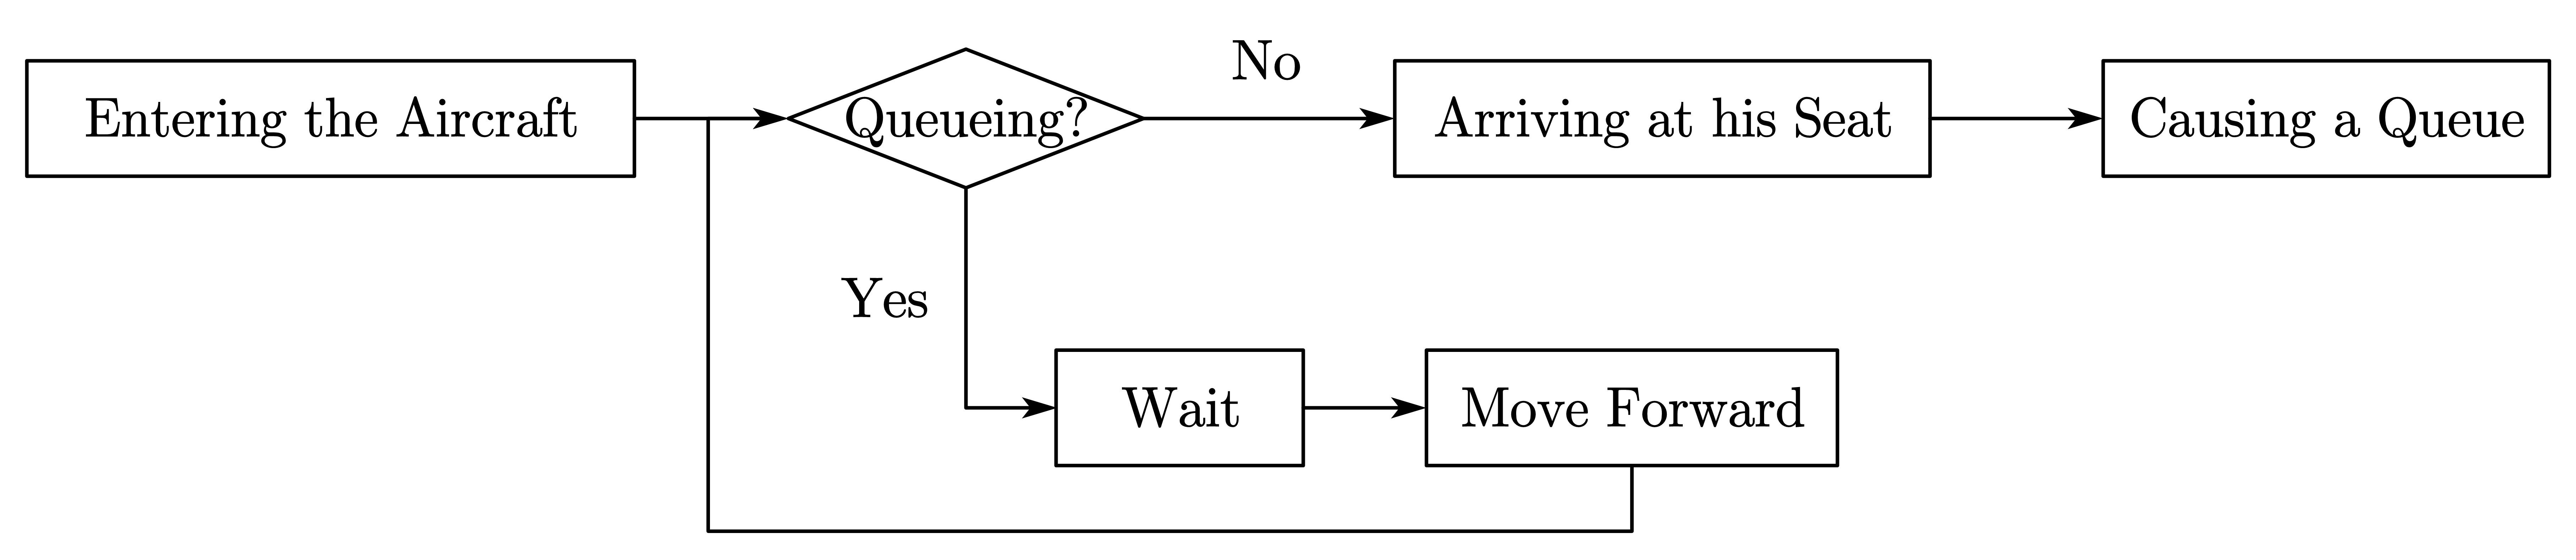
\includegraphics[width=14cm]{chart.jpg}

		\textit{Fig. 1 Boarding process of a specific passenger}
	\end{center}

	Moreover, it's important to note that if other seats have been occupied, its necessary for some passengers to stand up in order to provide unseated passengers with more space to reach their seat.

	In contradiction to the boarding process, the main problem of the disembarking process is that passengers who are eager to get out the plane may block the plane while they are taking their carry-on bags. This requires careful planning so that they will not stop the passengers on the back rows from moving.
	\subsection{Our Work}
	In our model, we need to find out the best strategy which suits the plane type perfectly. Therefore, our work is divided into 3 parts.
	\begin{itemize}
		\item Design a model which can calculate the time required to board and disembark when applied to all kinds of planes.
		\item Improve the model considering different situations and emergency events and design a brief strategy based on the results of our model.
		\item Apply our model to real-life planes and find out the best strategy which minimizes the boarding and disembarking time.
	\end{itemize}
	\subsection{General Assumptions}
	\begin{enumerate}
		\itembf{For each passenger, their luggage is put on the rack above them.}

		Airlines usually ensure this fact to minimize unnecessary congestion
		\itembf{For a certain passenger, the time to lay down his luggage and the time to remove it is the same.}

		This process can be mathematically acknowledged as \defword{reversible} (Consider when time relapses).
		\itembf{The total width of a passenger and his luggage is similar to the width between rows.}

		To provide the passengers the best flying experience, the flying company need to find a width between rows which will both satisfy the needs of people and maximize the plane's capacity.
		\itembf{All passengers walk in the same speed on the aisles.}

		Though there are energy difference caused by age and sex, there is slight difference of walking velocity when different passengers walk on a plane searching for their assigned seat. Therefore, we can neglect the difference and assume that all the passengers have the same ideal velocity.
		\itembf{Passengers never go backward.}

		Most passengers concentrated on finding their seat most. Therefore, they seldom miss their way and try to move backward.
		\itembf{First and business class passengers are prioritized with respect to those of the economic class.}

		Although (according to the ultimate results displayed in our essay), this is not the best boarding strategy for any types of plane and passengers, letting distinguished guests board first will give these passengers a sense of \defword{satisfaction} and enlarge the airline company's income. Therefore, we took this fact into consideration to make our model more realistic.
	\end{enumerate}
	\section{Model A: Math model and optimization for boarding and disembarking}
	\subsection{Model Overview}
	In this part, we will assess the plane and get the formulae desribing time sonsumption in boarding and disembarking. We define each seat as a block which has their own properties. All of the blocks belong to a coordinate divided accroding to the plane's overall arrangement. Later, we will get out the spent to move to these blocks also based on different moving conditions. We'll use these and the relavant optimization methods to derive the two types of \textit{best} solutions to airplane boarding schemes.
	\subsection{Assumptions}
	\begin{enumerate}
		\itembf{The luggage racks are designed to be adequate for any reasonable amount of luggage.}

		Consignment service is provided with the passengers before they enter the plane. Therefore, we can assume that there are enough space for the passengers to place smaller items, which means the space for storage is endless.
		\itembf{In a certain cell, $v$ is a fixed value.}

		Since $d$ (the width between rows, or the length of a cell) is taken as 0.8$\mathrm{m}$, a very small distance, there won't be a big difference in velocity change when a passenger is moving in the cell. Therefore, we can assume that $v$ in a certain block won't change.
		\itembf{There is enough space in the asile so that everty passenger can walk at their maximum speed.}

		To provide thier customers with the best flying experience, flying agencies usually make the aisle wide enough.  Therefore, we can assume that there is enough space for the passengers to miantain their speed.
	\end{enumerate}
	\subsection{Notice}
	In our model, we set \(\tau_0=1\mathrm{s}\) as the basic simulation unit, meaning that the model is also distrete. In an effort to standardize time and distance discretely, we make the following definitions in the rest of the model, (both \textit{time} and \textit{velocity} have no dimensions):
	\begin{itemize}
		\item \textbf{time}:
			For a period of \(t\,\mathrm{s}\) in \textit{SI}, we define the actual simulation time as \(t'=\dfrac{t}{\tau_0}\), which literally represents how many \(\tau_0\) s \(t\) consists of.
		\item \textbf{speed}:
			While a speed measuring \(v\,\mathrm{m\cdot s^{-1}}\) in reality means that the object travels \(v\,\mathrm{m}\) in a second, we define \defword{velocity} \(v'\) as the amount of \defword{time} (the \textit{time} here refers to the one as defined above) that takes the object to move \(d\), i.e. the length of a \textit{cell}. Therefore we have the following relationship between the two types of speeds:\[v=\dfrac{d}{v'\cdot \tau_0}\,\left(\mathrm{m\cdot s^{-1}}\right)\]
	\end{itemize}
	\subsection{Notations}
	We classify \textit{notations} into the following three types:
	\begin{itemize}
		\item \cA: won't change in the whole scope.
		\item \cB: may change in the whole scope, but won't change for a fixed set of passengers and a set plane.
		\item \varr: varies for different initial sequences of passengers.
	\end{itemize}
	\begin{center}
	\begin{tabular}{|l|l|l|l|}
		\hline
		$\tau_0$&simulation interval taken in our model, about \(1 \,\mathrm{s}\)&$\mathrm{s}$&\cA\\
		\hline
		\(\tau\)&simulation time step\(=\frac{\tau_0}{6}\)&\(\mathrm{s}\)&\cA\\
		\hline
		\(D\)&number of cells in the observable area, taken as \(4\,\left(\mathrm{persons}\right)\)&1&\cA\\
		\hline
		\(t\)&current time&1&\varr\\
		\hline
		$d$&width of each cell&$\mathrm{m}$&\cA\\
		\hline
		$N$&total number of passengers on the plane&1&\cB\\
		\hline
		$v_0$&maximum walking speed of a passenger aboard&1&\cA\\
		\hline
		$t_L (A)$&standard time for a passenger $A$ to place his luggage&1&\cA\\
		\hline
		$t_s$&time for a passenger to horizontally move a seat's length&1&\cA\\
		\hline
		$P$&the set of all passengers&/&\cB\\
		\hline
		$M$&number of cells on aisles&1&\cB\\
		\hline
		$C\left( A,t \right)$&the cell passenger $A$ is located at time $t$&1&\varr\\
		\hline
		$P_v\left( A \right)$&number of passengers visible within $D$ blocks before him&1&\varr\\
		\hline
		$S_i\left( A \right)$&total time needed to pass the first $i$ cells& 1&\varr\\
		\hline
		$v_i\left( A \right)$&the speed of passenger $A$ in the \(i^{\mathrm{th}}\) cell&1&\varr\\
		\hline
		$\tau _i\left( A \right)$&the time passenger $A$ spent in the $i^\text{th}$ cell&1&\varr\\
		\hline
		$v\left( A,t \right)$&the speed of passenger $A$ at $t$&1&\varr\\
		\hline
		$\gamma \left( A \right)$&non-compliance index of \(A\)&1&\cB\\
		\hline
		$l_i\left( A \right)$&whether the passenger $A$ is placing his luggage \(\in\left\{0,1\right\}\)&1&\varr\\
		\hline
		$\varepsilon \left( A \right)$&the time passenger $A$ need to be offered the seat&1&\varr\\
		\hline
		$\psi \left( A \right)$&time passenger $A$ to seat after starting putting luggage&1&\varr\\
		\hline
		$T\left( A \right)$&total boarding time of passenger $A$&1&\varr\\
		\hline
		$\Gamma$ &total boarding time&1&\varr\\
		\hline
	\end{tabular}
	\end{center}
	\subsection{Moving State of Passenger $A$}
	In this part, we mainly focus on how to describe the passengers. We saperate the plane into different \defword{cells}. Each cell has several properties describing its location, type (such as seats and aisles) and other properties. In special kinds of planes where the seats are arranged in irregular graphics, we still add them to the matrix, but we will not put them into consideration when it comes to calculations.

	First we will discuss the passenger's miving condition. To better describe the state of the seats, we define a simulating time step $\tau$, which equals $\dfrac{\tau_0}{6}$ ($\frac{1}{6}\mathrm{s}$). Under ideal circumstances, a passenger will move at a constant speed $v_0$. In our model, the smaller $v_0$ is, the faster the passenger travels.

	\begin{center}
		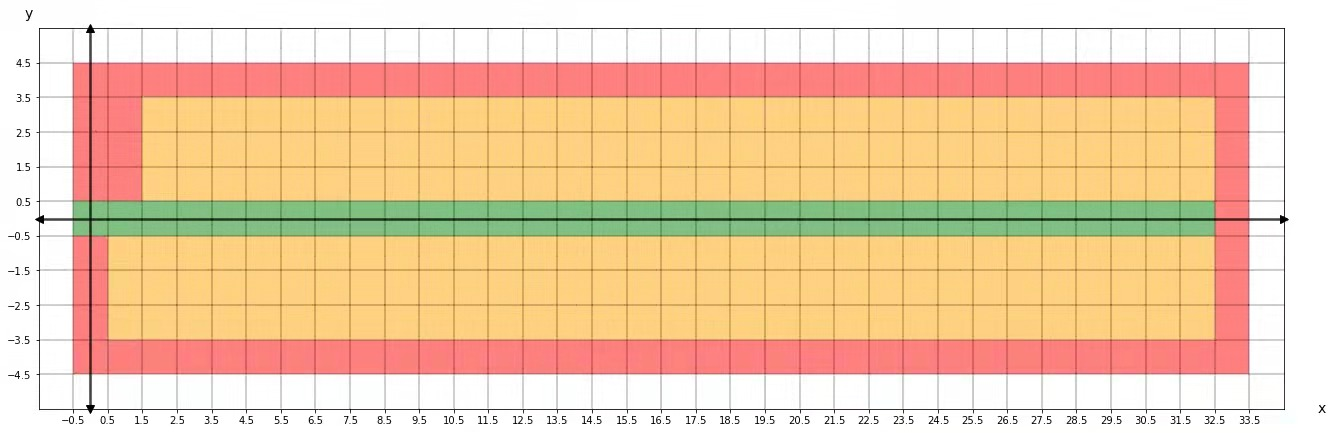
\includegraphics[width = 14cm]{cell_visualization.jpg}

		\small\textit{Fig. Construction of cells}
	\end{center}

	The following process will give the relationship solely between \(v\) in the aspect of both space and time.
	\subsubsection{Step One: \(v\to P_v\)}
	First, it's obvious that the more jammed a passenger is, the slower he or she moves. Therefore, it's important to first define \defword{density}.

	We define \defword{density} as the ratio of the number of people in the visible area to the number of cells in that visibility region. On an airplane, we take \textit{the number of cells in a passenger's visibility region} as \(4\), meaning that cells farther than that have no effects on the passenger. We have:
	\[\mathrm{Density\left(A\right)} = \dfrac{P_v\left(A\right)}{D}\]

	And according to the widely-adopted Greenshields speed-density linear model \cite{greenshields}, \[\mathrm{congested\:speed} = \mathrm{normal\:speed}\cdot\left(1-\mathrm{Density\left(A\right)}\right)\]

	By converting the physical \textit{velocity} into our unit, we have the following equation by definition:
	\[v(A)=\begin{cases}\dfrac{v_0}{1-\mathrm{Density\left(A\right)}}=\dfrac{v_0}{1-\frac{P_v\left(A\right)}{D}}, \text{if the passenger ahead is walking}\\\infty, \text{the passenger ahead stops}\end{cases}\]
d
	When \(v\left(A\right)=\infty\), the traditional way of calculation can no longer be used to calculate displacement. Therefore, we suppose that the passenger enters a state where he can't move until the person causing the queue gets seated. Currently we adopt the searching method to record that specific person, but later we will introduce a new concept \textit{cluster} to solve this problem.
	 After calculations, we've got the relationship between velocity and density.
	\subsubsection{Step Two: \(P_v\to \) passenger distribution}
	There clearly is a pretty logical way of ergodicing all the positions each time and get the respective \(P_v\left(A\right)\) for every passenger. But in order to achieve this with pure mathematics, we introduce the \textit{existence} factor and the \textit{effective} factor, both of which are included in the vector. Only when these two both have an effect on the passenger \(A\) can the index \(P_v\left(A\right)\) be taken into consideration.

	The first vector in the multiplication is the \textit{effective} factor, meaning that only people within the visibility range of \(A\) have an effect on him/her.

	\begin{center}
	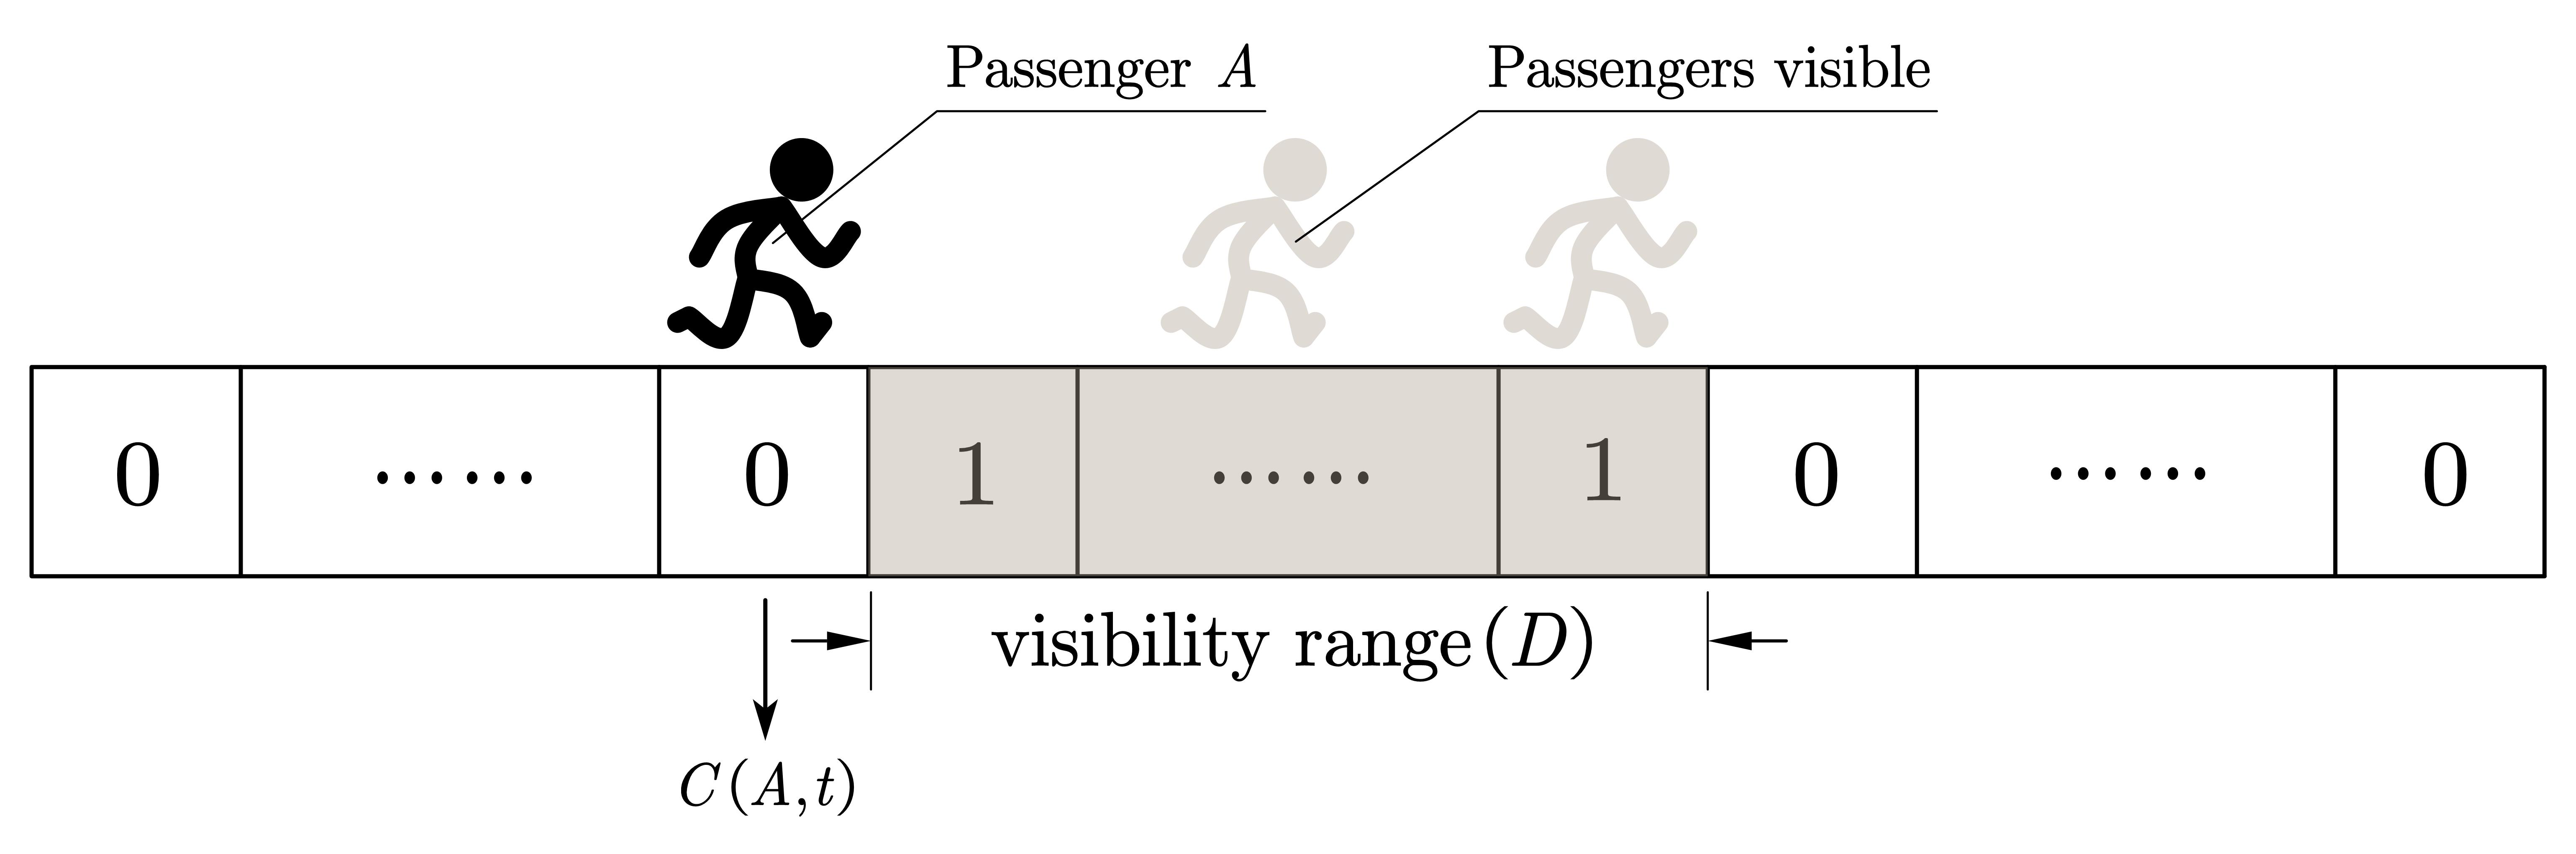
\includegraphics[width = 11cm]{effective factor.jpg}

	\small\textit{Fig. The effective factor}
	\end{center}

	The second vector is the \textit{existance} factor, indicating whether there exists anyone in each cell, which is also the \(0-1\) distribution for the whole group of cells. It can also be calculated by simply adding all the positions together.
	\[\text{Existance factor} = \text{Distribution of positions} = \sum\limits_{A\in P} \text{the position of }A\]

	By multiplying these two, we get the formula of \(P_v\left( A \right)\):

	$$P_v\left( A \right) =\left( 0,...0,\underset{D\:\mathrm{amount}\:\mathrm{of}\:1\mathrm{s}}{\underbrace{1,...,1}},0,...,0 \right) \times \left[ \sum_{A\in P}{\left( 0,...,0,\underset{\mathrm{the}\:C\left( A,t \right) ^{\mathrm{th}}\,\,\mathrm{position}\:\mathrm{from}\:\mathrm{top}\:\mathrm{to}\:\mathrm{bottom}}{\underbrace{1}},0,...,0 \right) ^{\top}} \right] $$
	\subsubsection{Step Three: passenger distribution \(\to \) individual \(v\)}
	According to our assumptions, it's easy to find that every passenger will move more slowly than the passenger ahead of him when they are in two adjacent cells. Therefore, each initial sequence yields a distinctive position set.

	We define \(S_i\left( A \right)\) as the time used to cover the distance of \(i\) cells:
	$$S_i\left( A \right) \xlongequal{\mathrm{def}}\sum_{j=1}^i{v_j\left( A \right)}>0$$

	With the formula above, it's easy to determine the current cell of \(A\):
	$$C\left( A,t \right) =\min_{\substack{\frac{t}{S_i\left( A \right)}\le 1\\1\le i\le M\\}} \left\{ i \right\} $$
	(In this model, $C(A,t)$ can be considered as a linear combination of $v$.)
	\subsubsection{Final Step: \(v\to v\)}
	Summing up the previous three parts, we can identify $v(A,t)$, which is demonstrated in the following formulae:
	$$v\left( A_l,t \right) =\frac{v_0}{E_l+\sum\limits_{\alpha =1}^N{\left( \sum\limits_{\beta =1}^T{\left( \lambda _{\alpha ,\beta}^{\left( l \right)}\cdot v\left( A_{\alpha},\beta \right) \right)} \right)}}\left( l\in \left\{ 1,2,...,N \right\} ,E_l\in \mathbb{R} \right)$$
	where
	$$\sum_{\alpha =1}^N{\left( \sum_{\beta =1}^T{\left( \lambda _{\alpha ,\beta}^{\left( l \right)}\cdot v\left( A_{\alpha},\beta \right) \right)} \right)}=\frac{v_0}{v\left( A_l,t \right)}-E_l\left( l\in \left\{ 1,2,...,N \right\} ,E_l\in \mathbb{R} \right)$$
	is a linear combination of the velocities, also indicating that with the set of all possible previous velocities given, we can use this recursion algorithm to calculate the velocity at the next time step. (Notice that not only process three but also the first two steps ensure linearity, and that the \(\lambda\,\)s are independent from the previous \(v\,\)s.)
	\subsubsection{Putting luggage and Offering seats}
	Next we calculate the time spent while one is trying to take his/her seat.
	\begin{itemize}
		\item \defword{\textbf{Stowing luggage.}}

		The standard stowing time has already been given as \(t_L\). However, the time does not always remain unvariant. Due to the fact that different passengers bring different amounts of luggage aboard and that some passengers disobey boarding rules, we introduce a non-compliance index \(\gamma\left(A\right)\). The higher \(\gamma\left(A\right)\) is, the more time it takes \(A\) to stow his/her luggage.

		Therefore, the overall time \(A\) consumed to stow his/her luggage equals:
		\[\text{stowing time}=\gamma \left( A \right) t_L \]
		\item \defword{\textbf{Getting seated.}}

		In some strategies, passengers near the aisle have to stand up to let a new traveller get through. (In other strategies such as \textit{window middle aisle}, this scenario never occurs). We add a special property to each cell which determines whether the cell is being seated. When the passenger outside has been seated and the other two passengers inside come, the passenger needn't stand up twice to offer his seat. Therefore, we can describe the time spent in seating as:
		$$t(1,k)=v_0$$
		$$t(A,a)=\begin{cases}t(A-1,a+1),\text{there is a person on the $a+1$ block}\\v_0, \text{the \textbf{a+1} block is empty}\end{cases}$$

		To form equations, we adopt motional physics and according to our assumptions, the time consumed to offer seat is proportional to the distance one moves, which is then proportional to the number of seats separating one from the aisle.
		\begin{center}
		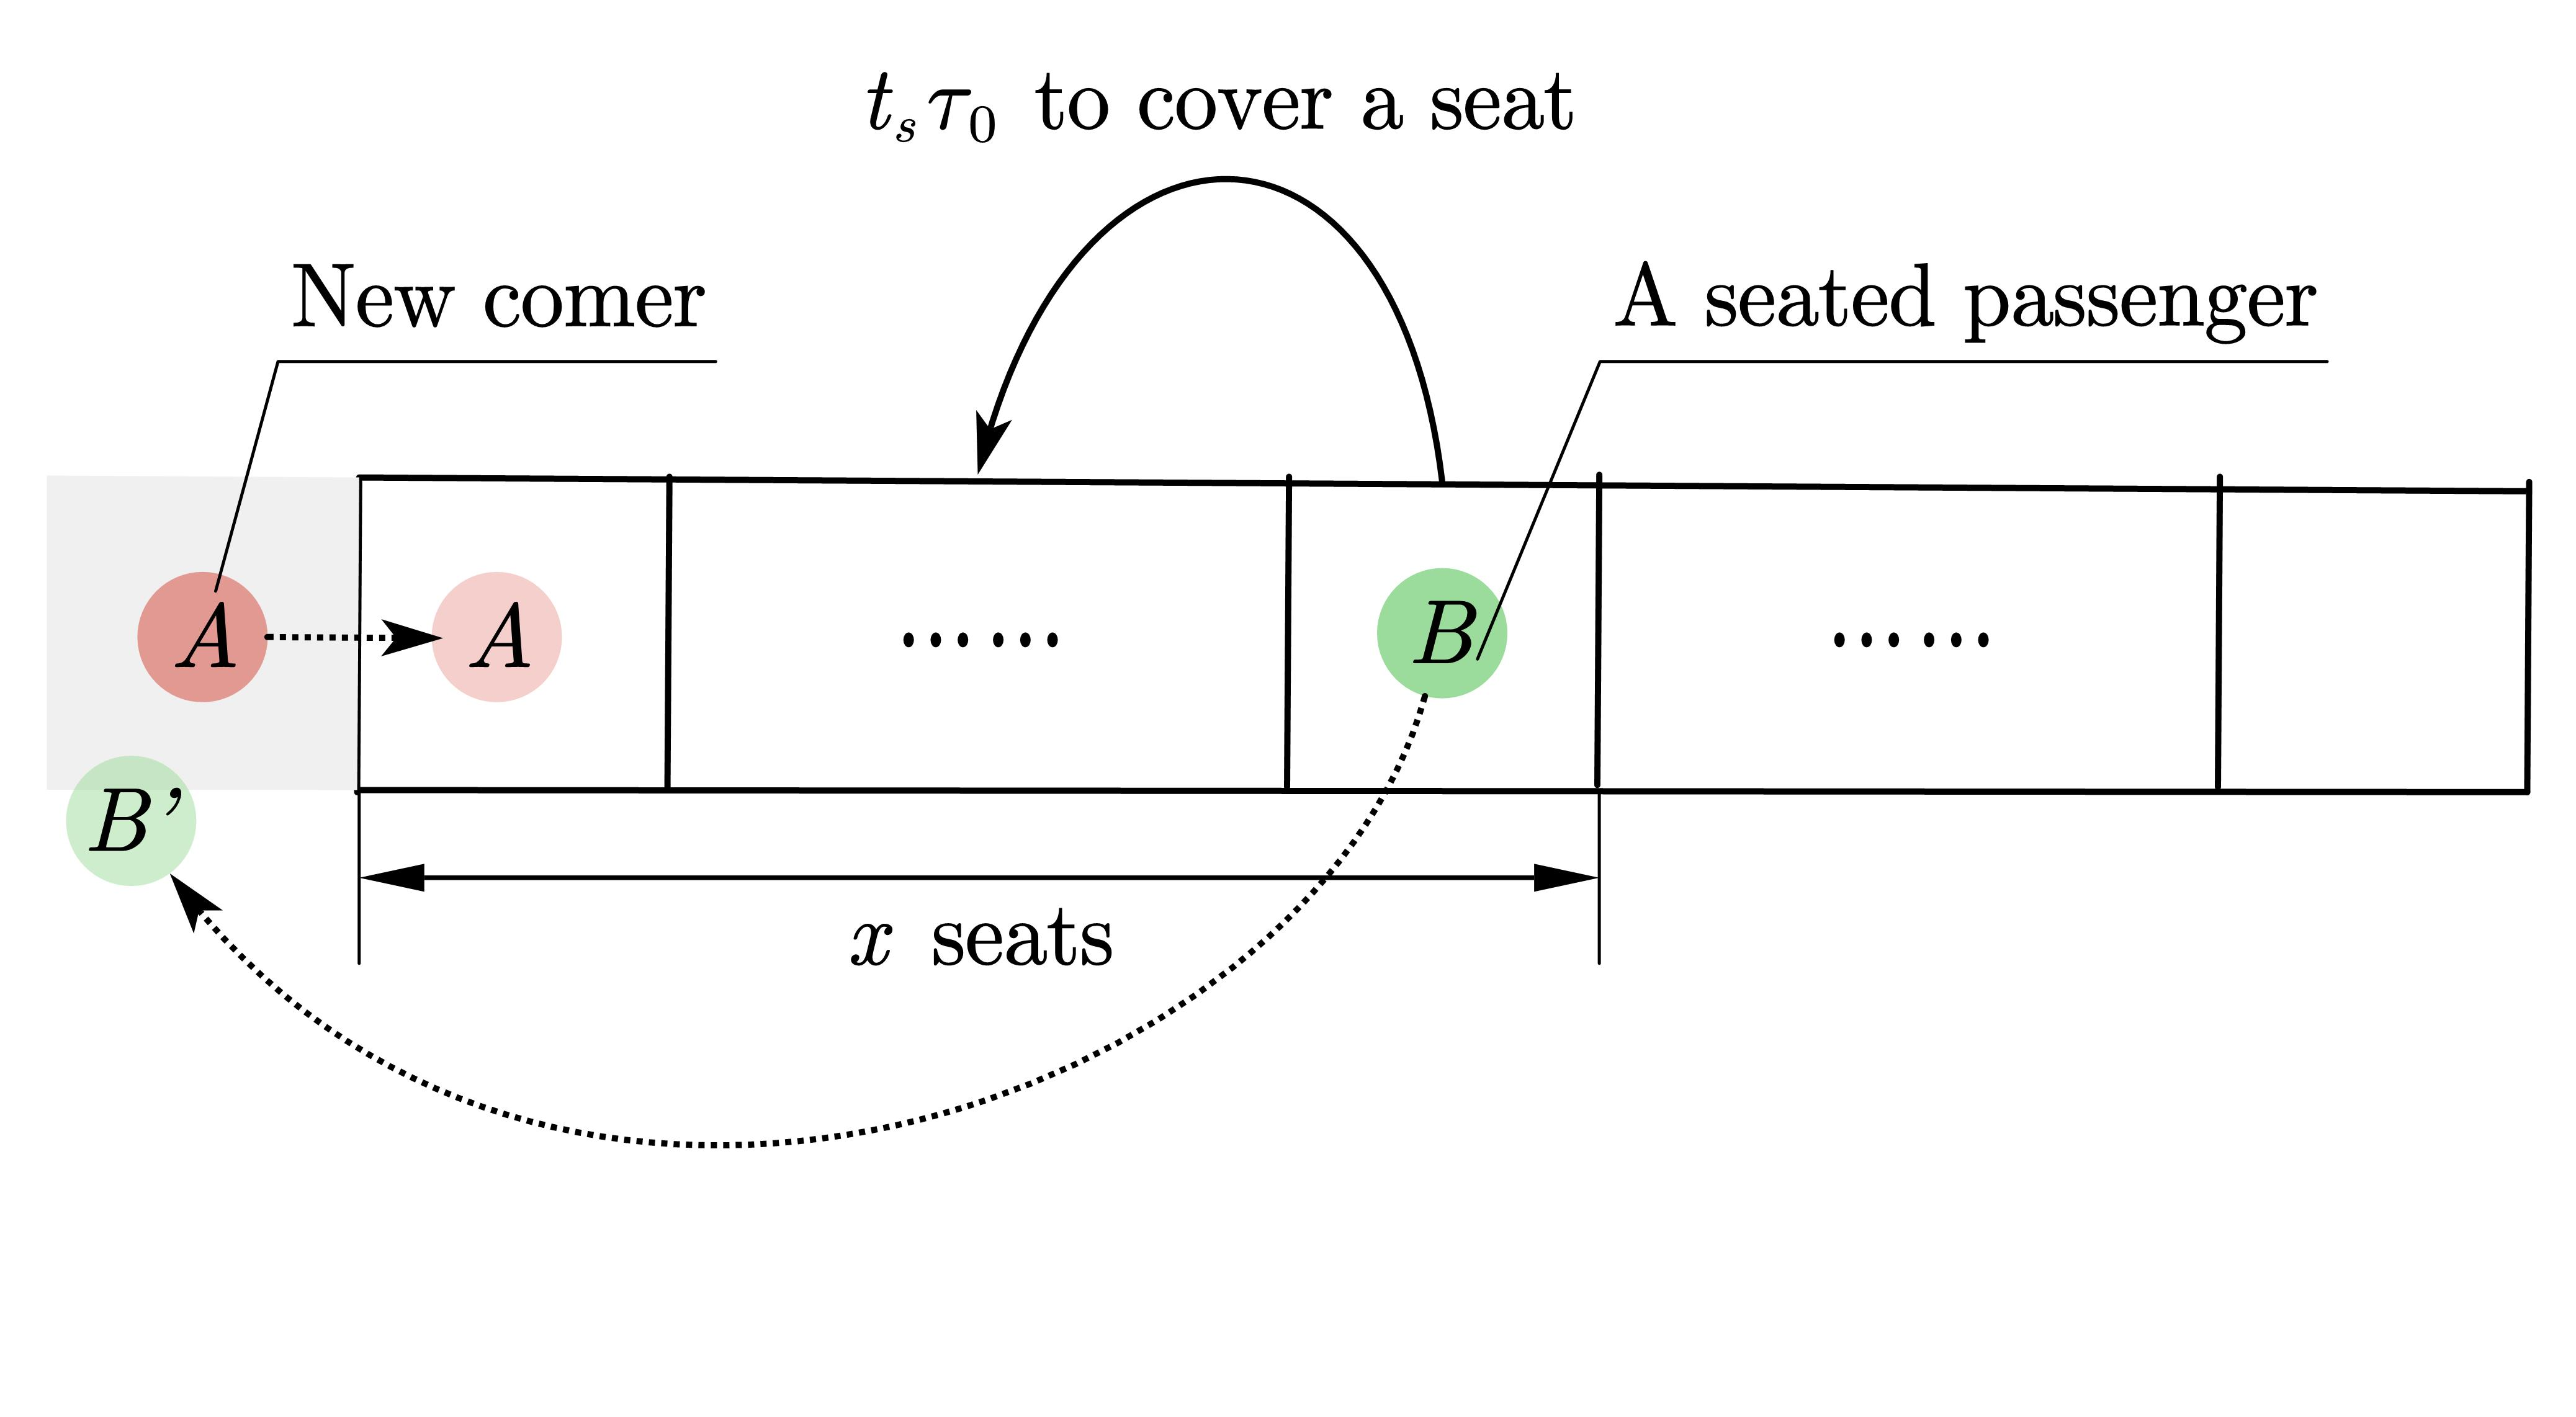
\includegraphics[width = 10cm]{offering a seat.jpg}

		\small\textit{Fig. Offering a seat}
		\end{center}

		So when he/she travels $x$ cells, the total time \(B\) consumed equals:
		$$t(B)=x\cdot t_s \cdot \tau_0$$

		And we take the maximum of the time to offer seats in this line as the total:
		\[\text{time to offer seat}=\max\limits_{B\in \text{this line}}\left\{t(B)\right\} = \max\limits_{B\in \text{this line}}\left\{x_{B}\cdot t_s \cdot \tau_0\right\}\]

		Once the passenger takes his/her seat, the cell on the aisle is no longer occupied, which ends the queuing process.
	\end{itemize}
	We introduce a special variable $l_i(A)$ to describe the passengers state. If he stops to place his luggage, \(l_i(A)=1\). Conversely, \(l_i(A)=0\). Below is given the two types of states of passenger \(A\):
	\[\Xi_i\left(A\right)=\left( \begin{matrix}
	l_i\left( A \right)&		\\
	&		1-l_i\left( A \right)\\
	\end{matrix} \right) \in \mathbb{R}^2\cap \left\{ \left( \begin{matrix}
	0&		\\
	&		1\\
	\end{matrix} \right) ,\left( \begin{matrix}
	1&		\\
	&		0\\
	\end{matrix} \right) \right\}\]

	In additon, we define $\psi(A)$ to descibe the total time passenger $A$ spent from stopping placing his luggage to sitting down. It is clear that $\psi \left( A \right) =\max \left\{ \epsilon \left( A \right) ,\gamma \left( A \right) t_L \right\}$.

	\subsubsection{Calculating total time}
	Next, we calculate the total time a passenger spends in cell \(i\) with the previous parts combined. This can be done through adding those together. Therefore, we can define the time passenger $A$ spent in the $i^\text{th}$ cell as:
	$$\tau _i\left( A \right) =v_i\left( A \right) +l_i\left( A \right) \cdot \psi \left( A \right) +\underset{\mathrm{whether}\:\:\mathrm{he}/\mathrm{she}\:\:\mathrm{needs}\:\:\mathrm{to}\:\:\mathrm{queue}}{\underbrace{\left( 1-l_i\left( A \right) \right) }}\cdot \psi \left( \mathrm{queuing}\:\:\mathrm{origin} \right)$$
	or in other words:
	\[\Xi _{\mathrm{full}\:\mathrm{state}}=\left( \begin{matrix}
	v_i\left( A \right)&		\\
	&		\Xi _i\left( A \right)\\
	\end{matrix} \right) \times \left( \begin{matrix}
	\text{whether moving}&		&		\\
	&		\text{whether stowing}&		\\
	&		&		\text{whether waiting}\\
	\end{matrix} \right) \]

	Finally, we can get the total time $A$ spent in boarding $T(A)$:
	$$T\left( A \right) =\sum_{i=1}^M{\tau _i\left( A \right)}$$
	(If $i$ is beyond \(A\)'s target, $\tau_i(A)=0$)

	And by calculating the total boarding time of each passenger and put them in order, we can find out:
	$$\Gamma =\max_{1\le i\le N} \left\{ T\left( A_i \right) \right\}$$
	\subsection{Optimization}
	In this part, we'll use various mathematical methods to give the fastest possible boarding strategy.
	\subsubsection{Parallel boarding}
	We noticed that the passengers in the rows in the left and those in the rows in the left wouldn't disrupt each other, for they do not share much space of the aisles. So a good strategy is to board some passengers in the left and some in the right at the same time. However, if we arrange the order strictly from the two sides to the middle, there would be too much queuing in the middle rows.

	To reduce the queuing, we can first divide the aircraft into eight groups of seats, each of which contains three rows. Then, we can board passengers in group $n$ and group $n+4$ together. This would not cause much queuing, and can also maximize efficiency by \defword{parallel boarding}.

	We define the \defword{parallelity index} \(r\) as the portion of cells that are in the stowing state to the number of total aisle cells inside the plane: (In the first example, for instance, this total number equals \(33\).)
	\[r\left(t\right) = \dfrac{\#\text{cells in stowing state}}{\#\text{cells inside the plane}}\ddef\dfrac{C_s}{C_p}\]

	In intuition, the fastest strategy comes when everyone is blocked by one queuing origin each time, meaning that there may be \(C_s=C_p\) passengers stowing luggage but only costs a total of \(1\times t_L+o\left(1\right)\) amount of time, where \(o(1)\) is a constant relyin only on the passenger set and the plane type, which can greatly help reduce total time. To prove this, we use the attributes of discrete optimizations and get the aids from the computer.
	\begin{center}
		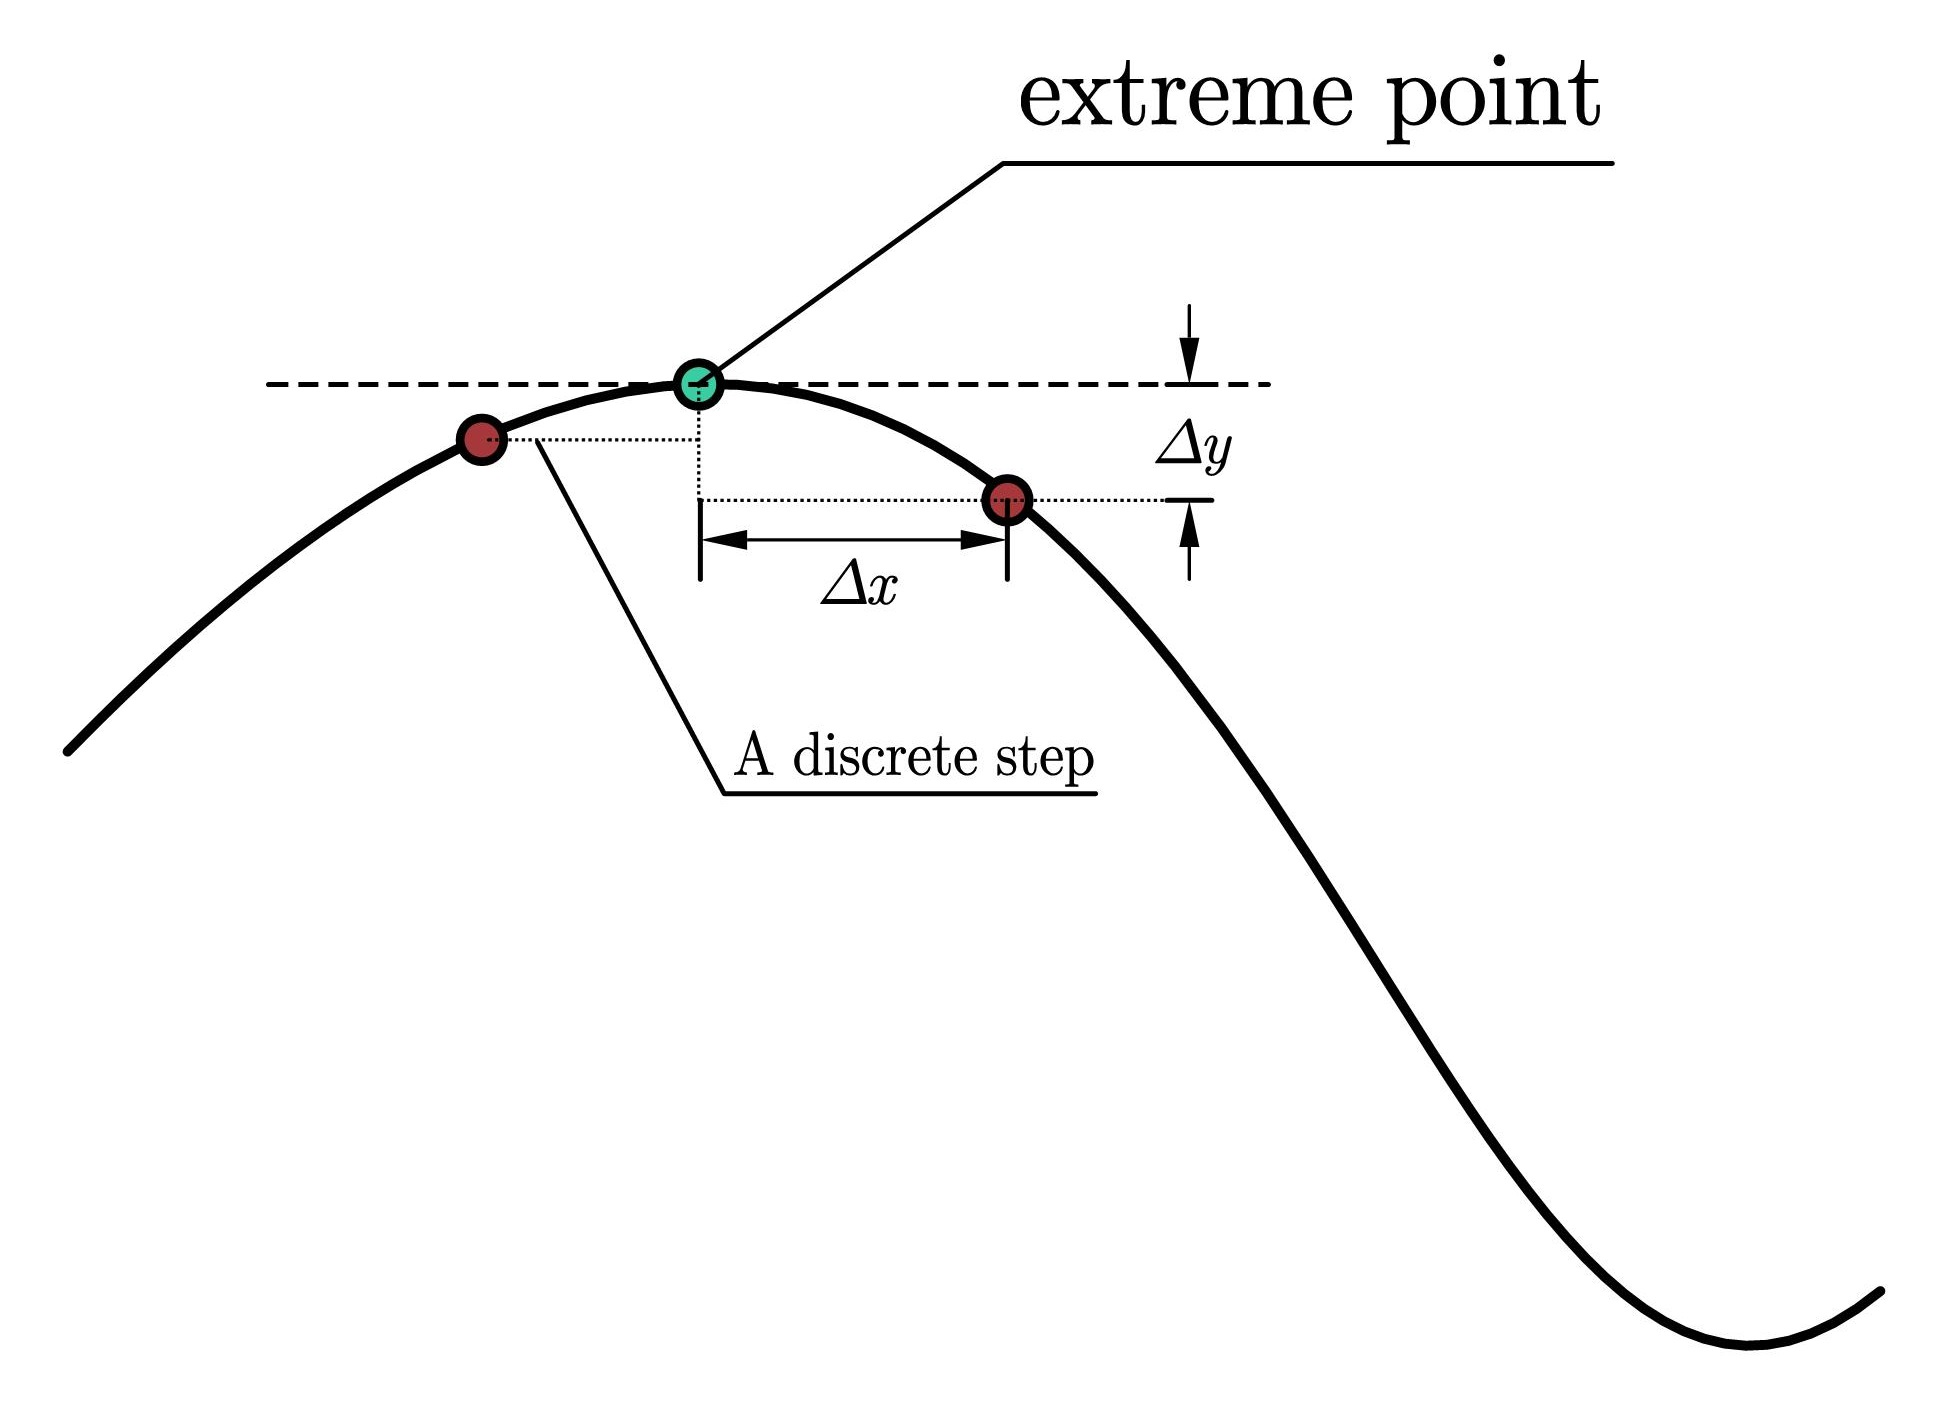
\includegraphics[height = 5cm]{discrete optimization.jpg}

		\small\textit{Fig. Discrete optimization}
	\end{center}

	\subsubsection{Computer-aided optimization}
	After adopting the discrete optimization model and with the \defword{parallel} nature, we get the following ideal boarding plans:

	\begin{center}
		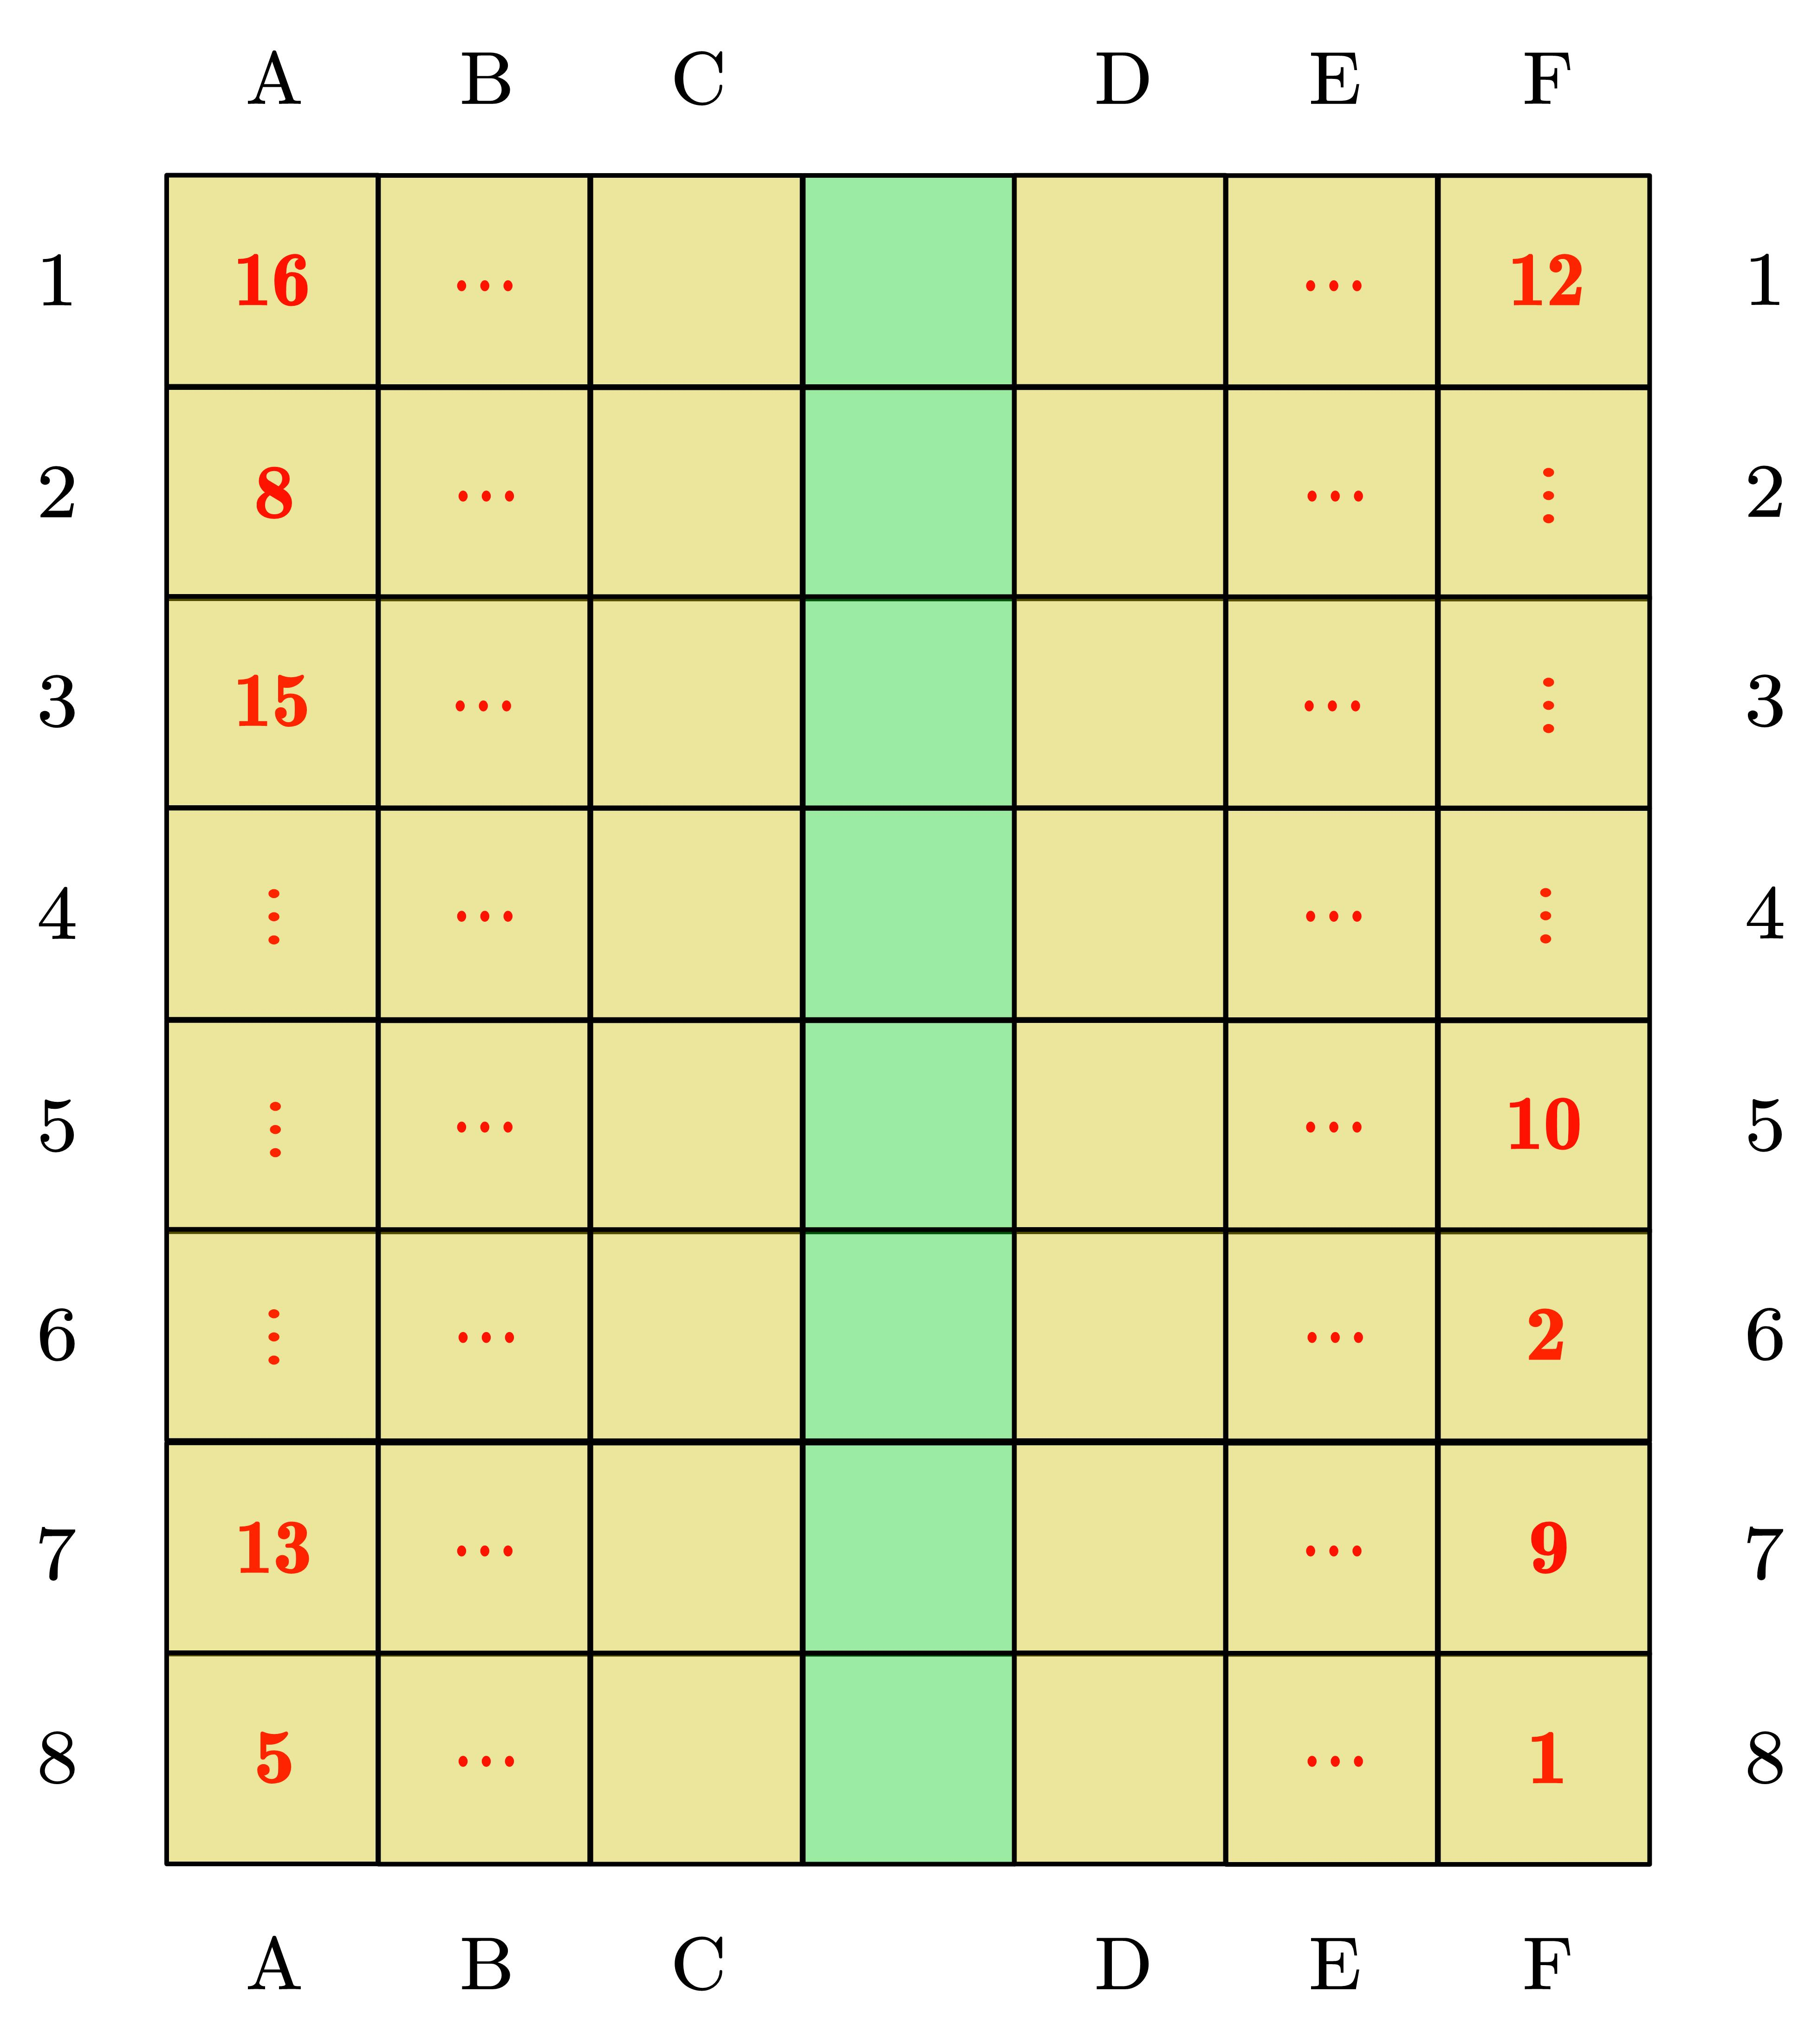
\includegraphics[height =4cm]{steffen1.jpg}
		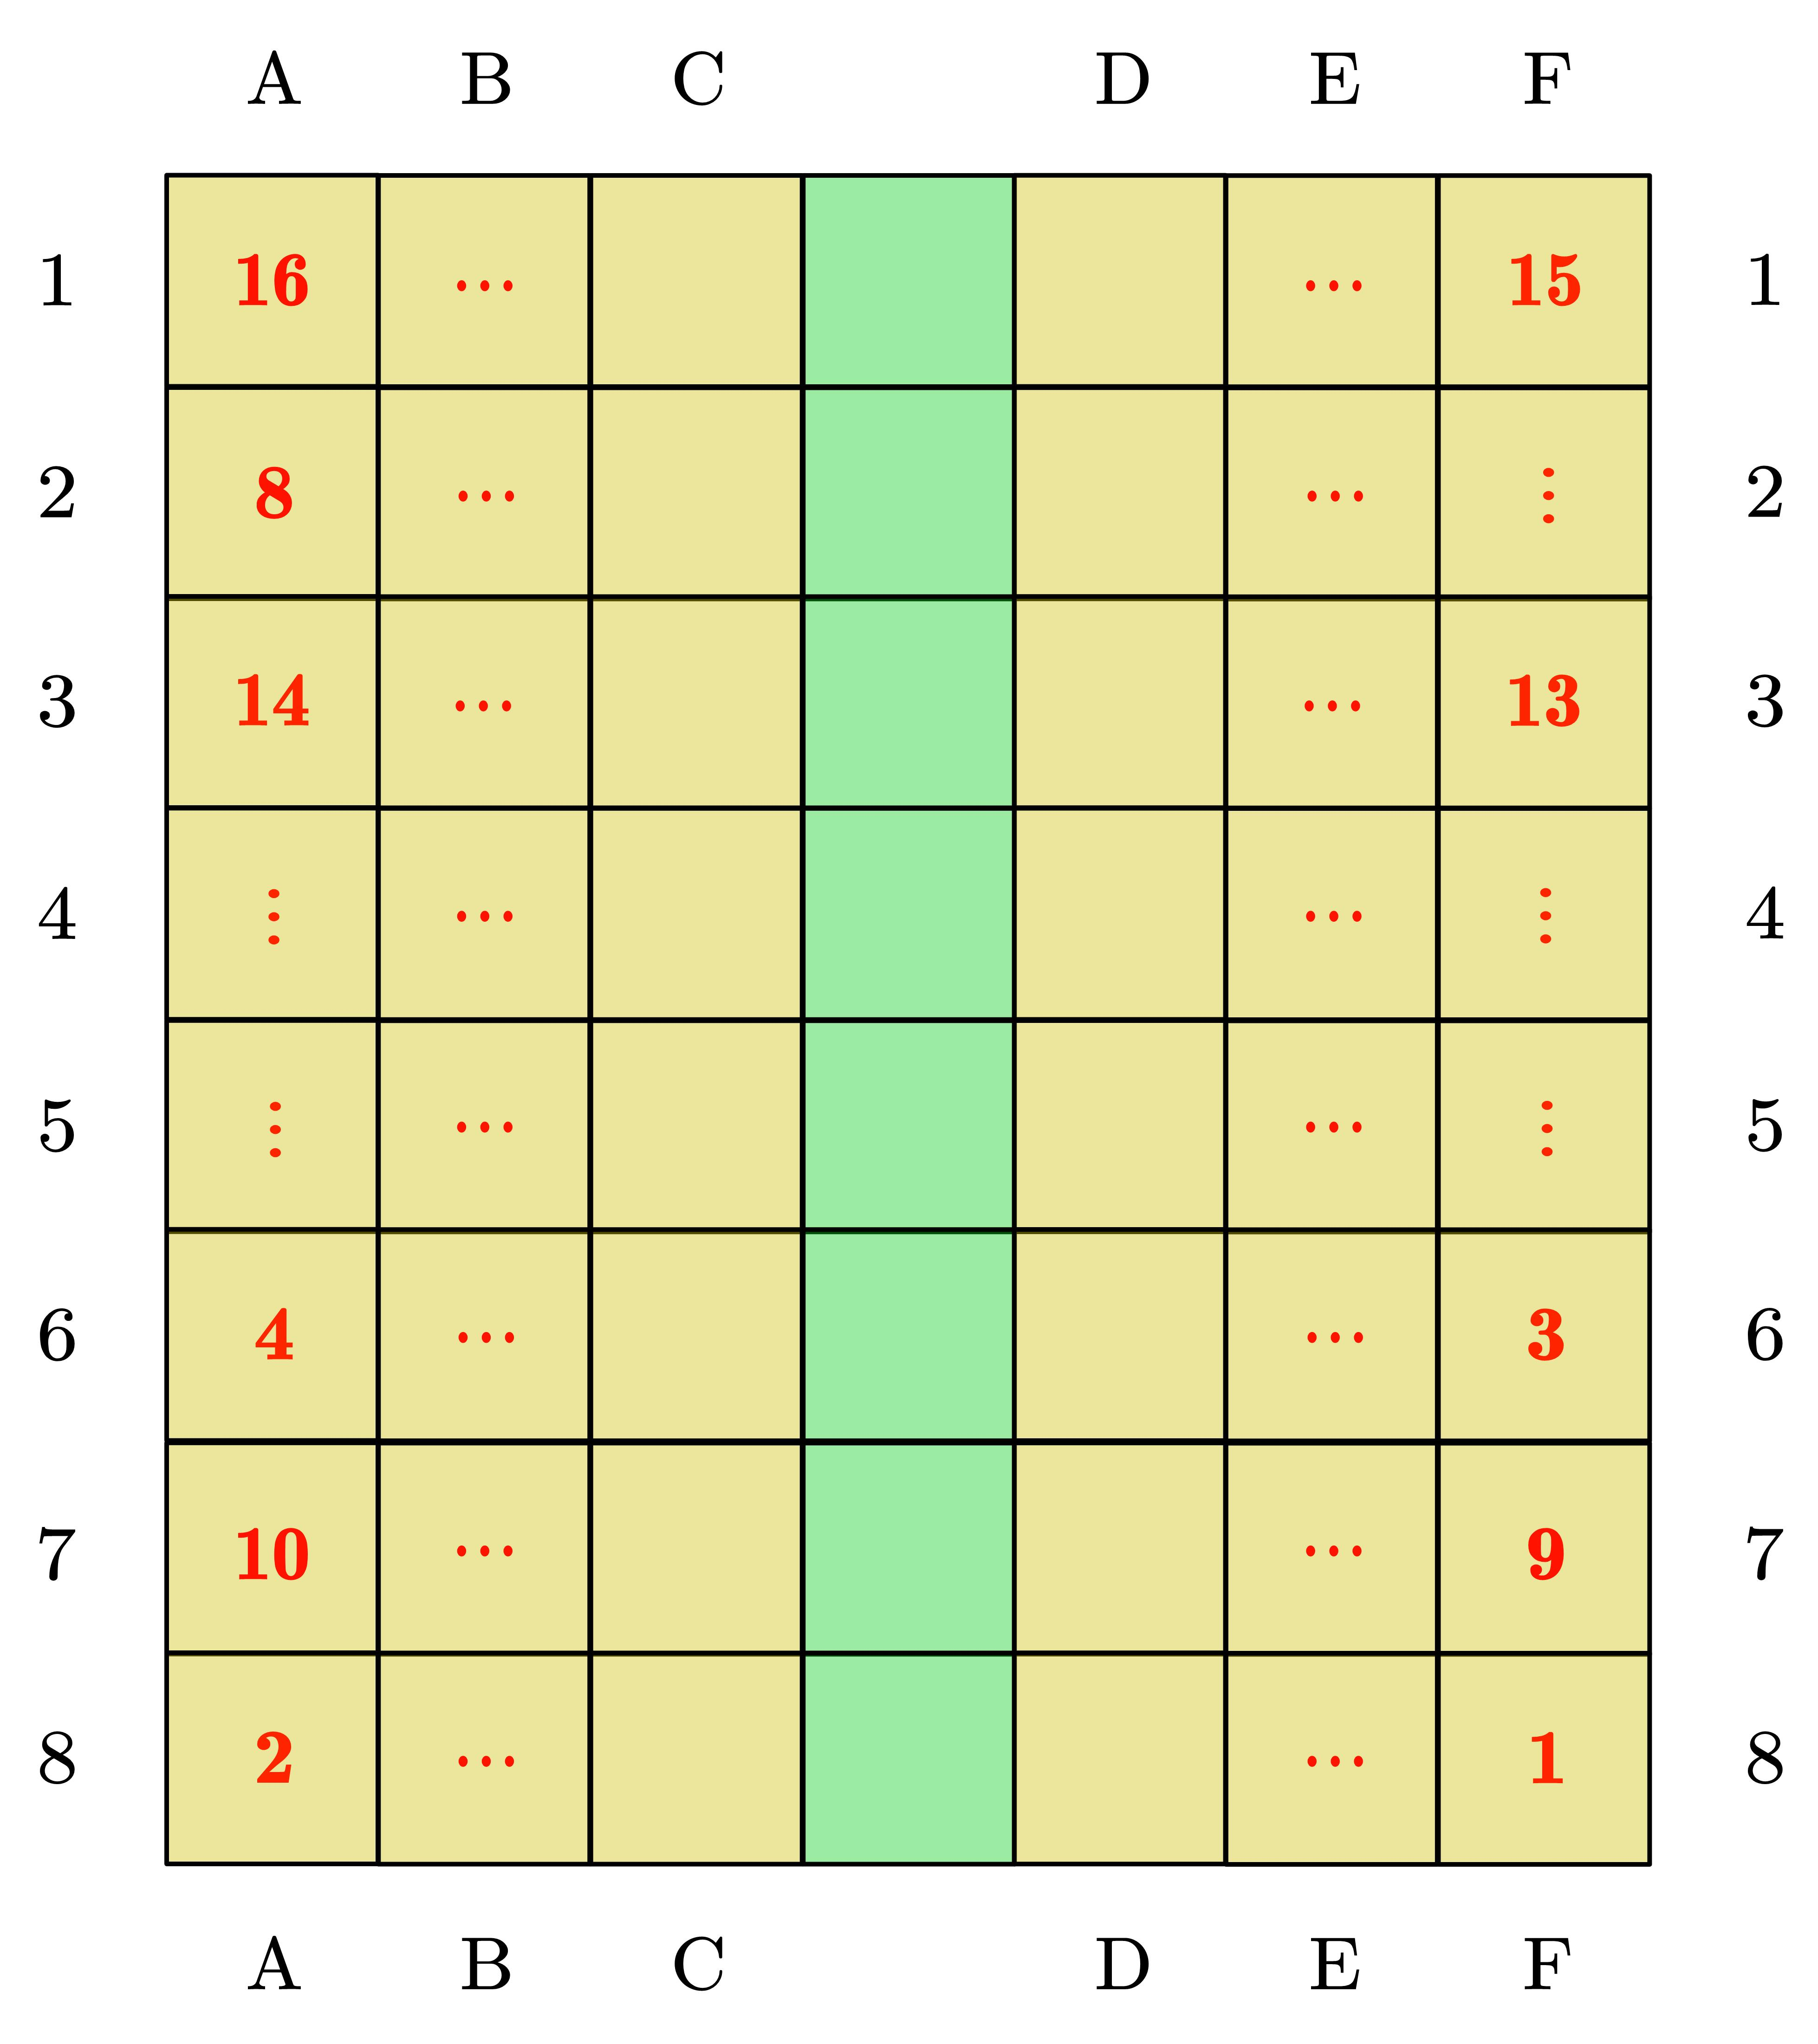
\includegraphics[height = 4cm]{steffen2.jpg}

		\small\textit{Fig. Two ideal boarding plans}
	\end{center}

	\textbf{Note. }Later, we'll use our previous mathematical model to verify our solutions and also calculate the relavant \defword{satisfactory} index, which will be included in the subsequent section. Here, we present the calculated optimum in advance to display its parallelity.
	\subsection{Disembarking of passenger $A$}
	The conclusions drawn in the boarding model can also be applied to the disembarking process, where the only difference is that passengers can get their luggage while travellers in the prior sequence have just passed through the aisle.
	\\ \\
	\textbf{Claim 1.} On whatever occasions, the best strategy always comes when the aisle is consistently full (if possible in reality).
	\\ \\
	\textbf{Proof of Claim 1.} We use the idea of adjustment in our proof. Suppose at time \(t\), passengers in the queue range from \(B_1\) to \(B_x\), and that \(P_\mathrm{next}\) is a subsequent set of passengers starting from \(B_1\) and owns these properties:
	\begin{enumerate}
		\item \(P_{\mathrm{next}}=\left\{ B_1,...,B_y \right\} ,\,\,y\in \left\{ 1,2,...,x \right\} \), which means that \(P_{\mathrm{text}}\) contains a series of subsequent passengers starting from \(B_1\).
		\item \(\forall i\in \left\{ 1,2,...,y-1 \right\} ,\:\:C\left( B_i,t \right) \:\mathrm{is}\:\mathrm{next}\:\mathrm{to}\:C\left( B_{i+1},t \right) \), meaning that the queue fits all the \(y\) squares starting from \(B_1\).
		\item \(\mathrm{if}\:B_{y+1}\:\mathrm{exists},\:\mathrm{then}\:C\left( B_y,t \right) \:\mathrm{is}\:\mathrm{not}\:\mathrm{next}\:\mathrm{to}\:C\left( B_{y+1},t \right) \), meaning that \(P_{\mathrm{next}}\) is the longest \textit{sub-queue} which follows property \(2\).
	\end{enumerate}

	Now, if \(B_{y+1}\) doesn't exist, then we've proven our \textbf{Claim 1}. (because passengers can not get close any further since there is no space between them.) Suppose there exists \(B_{y+1}\), and according to property \(3\), we can assure that there certainly exists a time $\Delta\tau$ for \(B_{y+1}\) to get coincidenced with the cell right behind \(B_y\), covering distance \(\Delta d\). Now, as an ideological experiment, let's move passengers \(B_{y+1},B_{y+2},...,B_x\) foward by \(\Delta d\), and it's obvious that each passenger are saved \(\Delta \tau\) time needed to \textit{keep up with} the set \(P_{\mathrm{next}}\).

	\begin{center}
		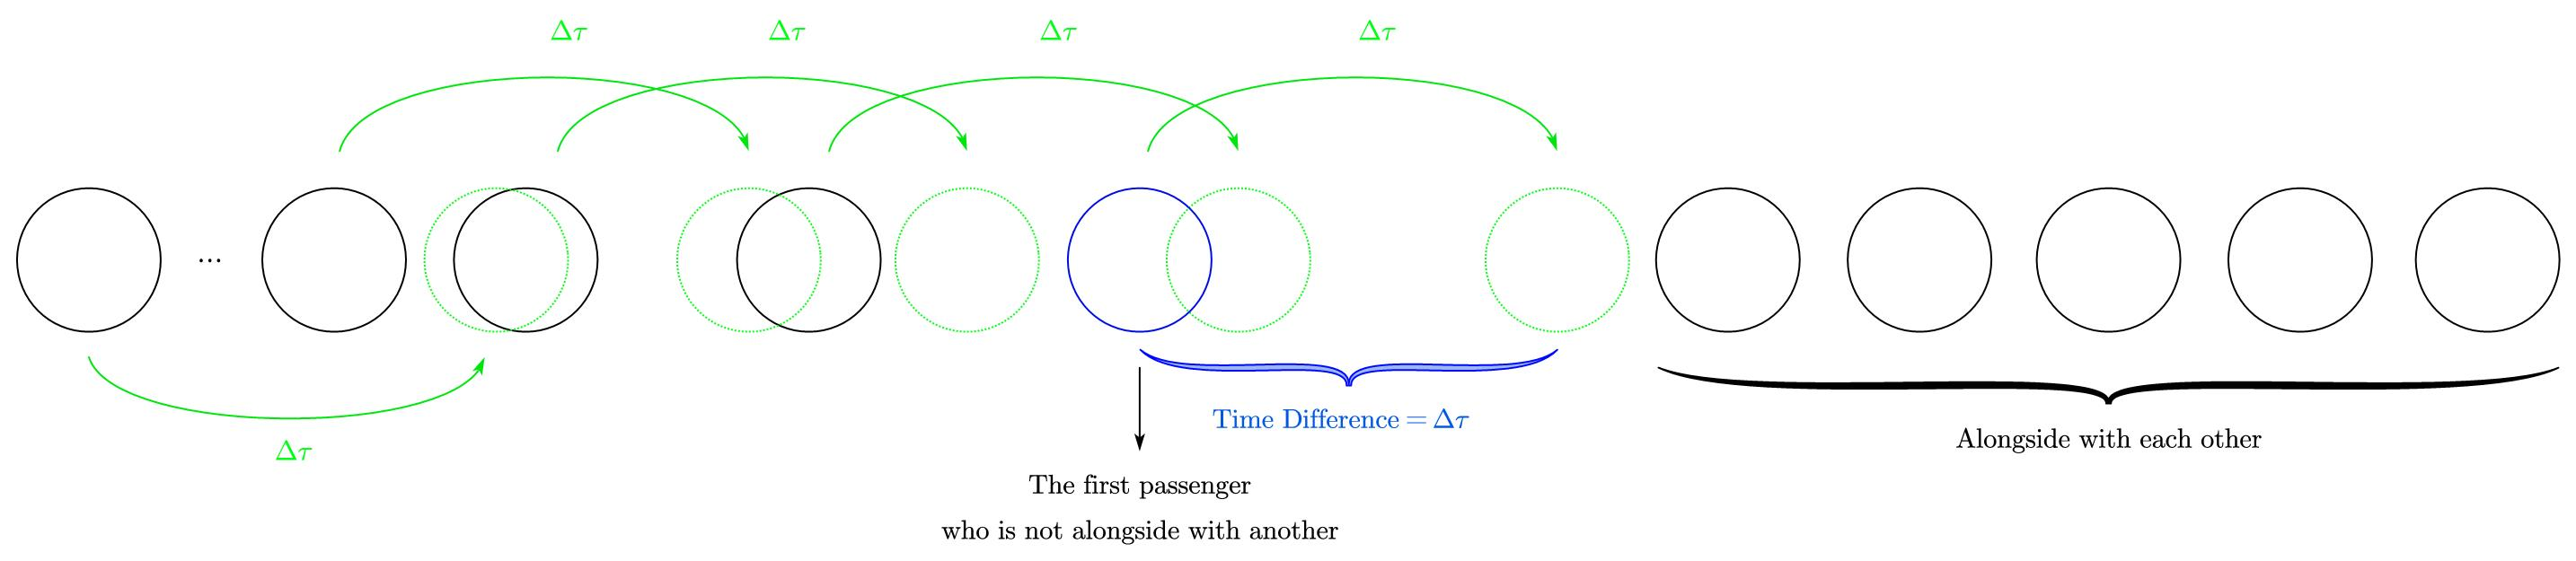
\includegraphics[width = 14cm]{display of Delta tau.jpg}

		\small\textit{Fig. Visualization of the actions}
	\end{center}

	According to \textbf{Claim 1}, we can find that:
	$$\text{the best disembarking strategy}\Leftrightarrow
	\text{let all the passengers become a row}$$

	So we can find that:
	$$\Gamma_\text{disembarking}=\text{boarding time of a line of the same amount of passengers}+t_L(A)$$

	Now the question comes to how to reorder the passengers. We let the passengers who sit near the passengers enter the aisle first. After the first people get the luggage, the people who sits next to him will get prepared to enter the aisle. To sum up, we can get the image below which best explains our strategy. And the strategy itself also ensures that the aisle is always \textit{positively} filled with passengers.

	\begin{center}
		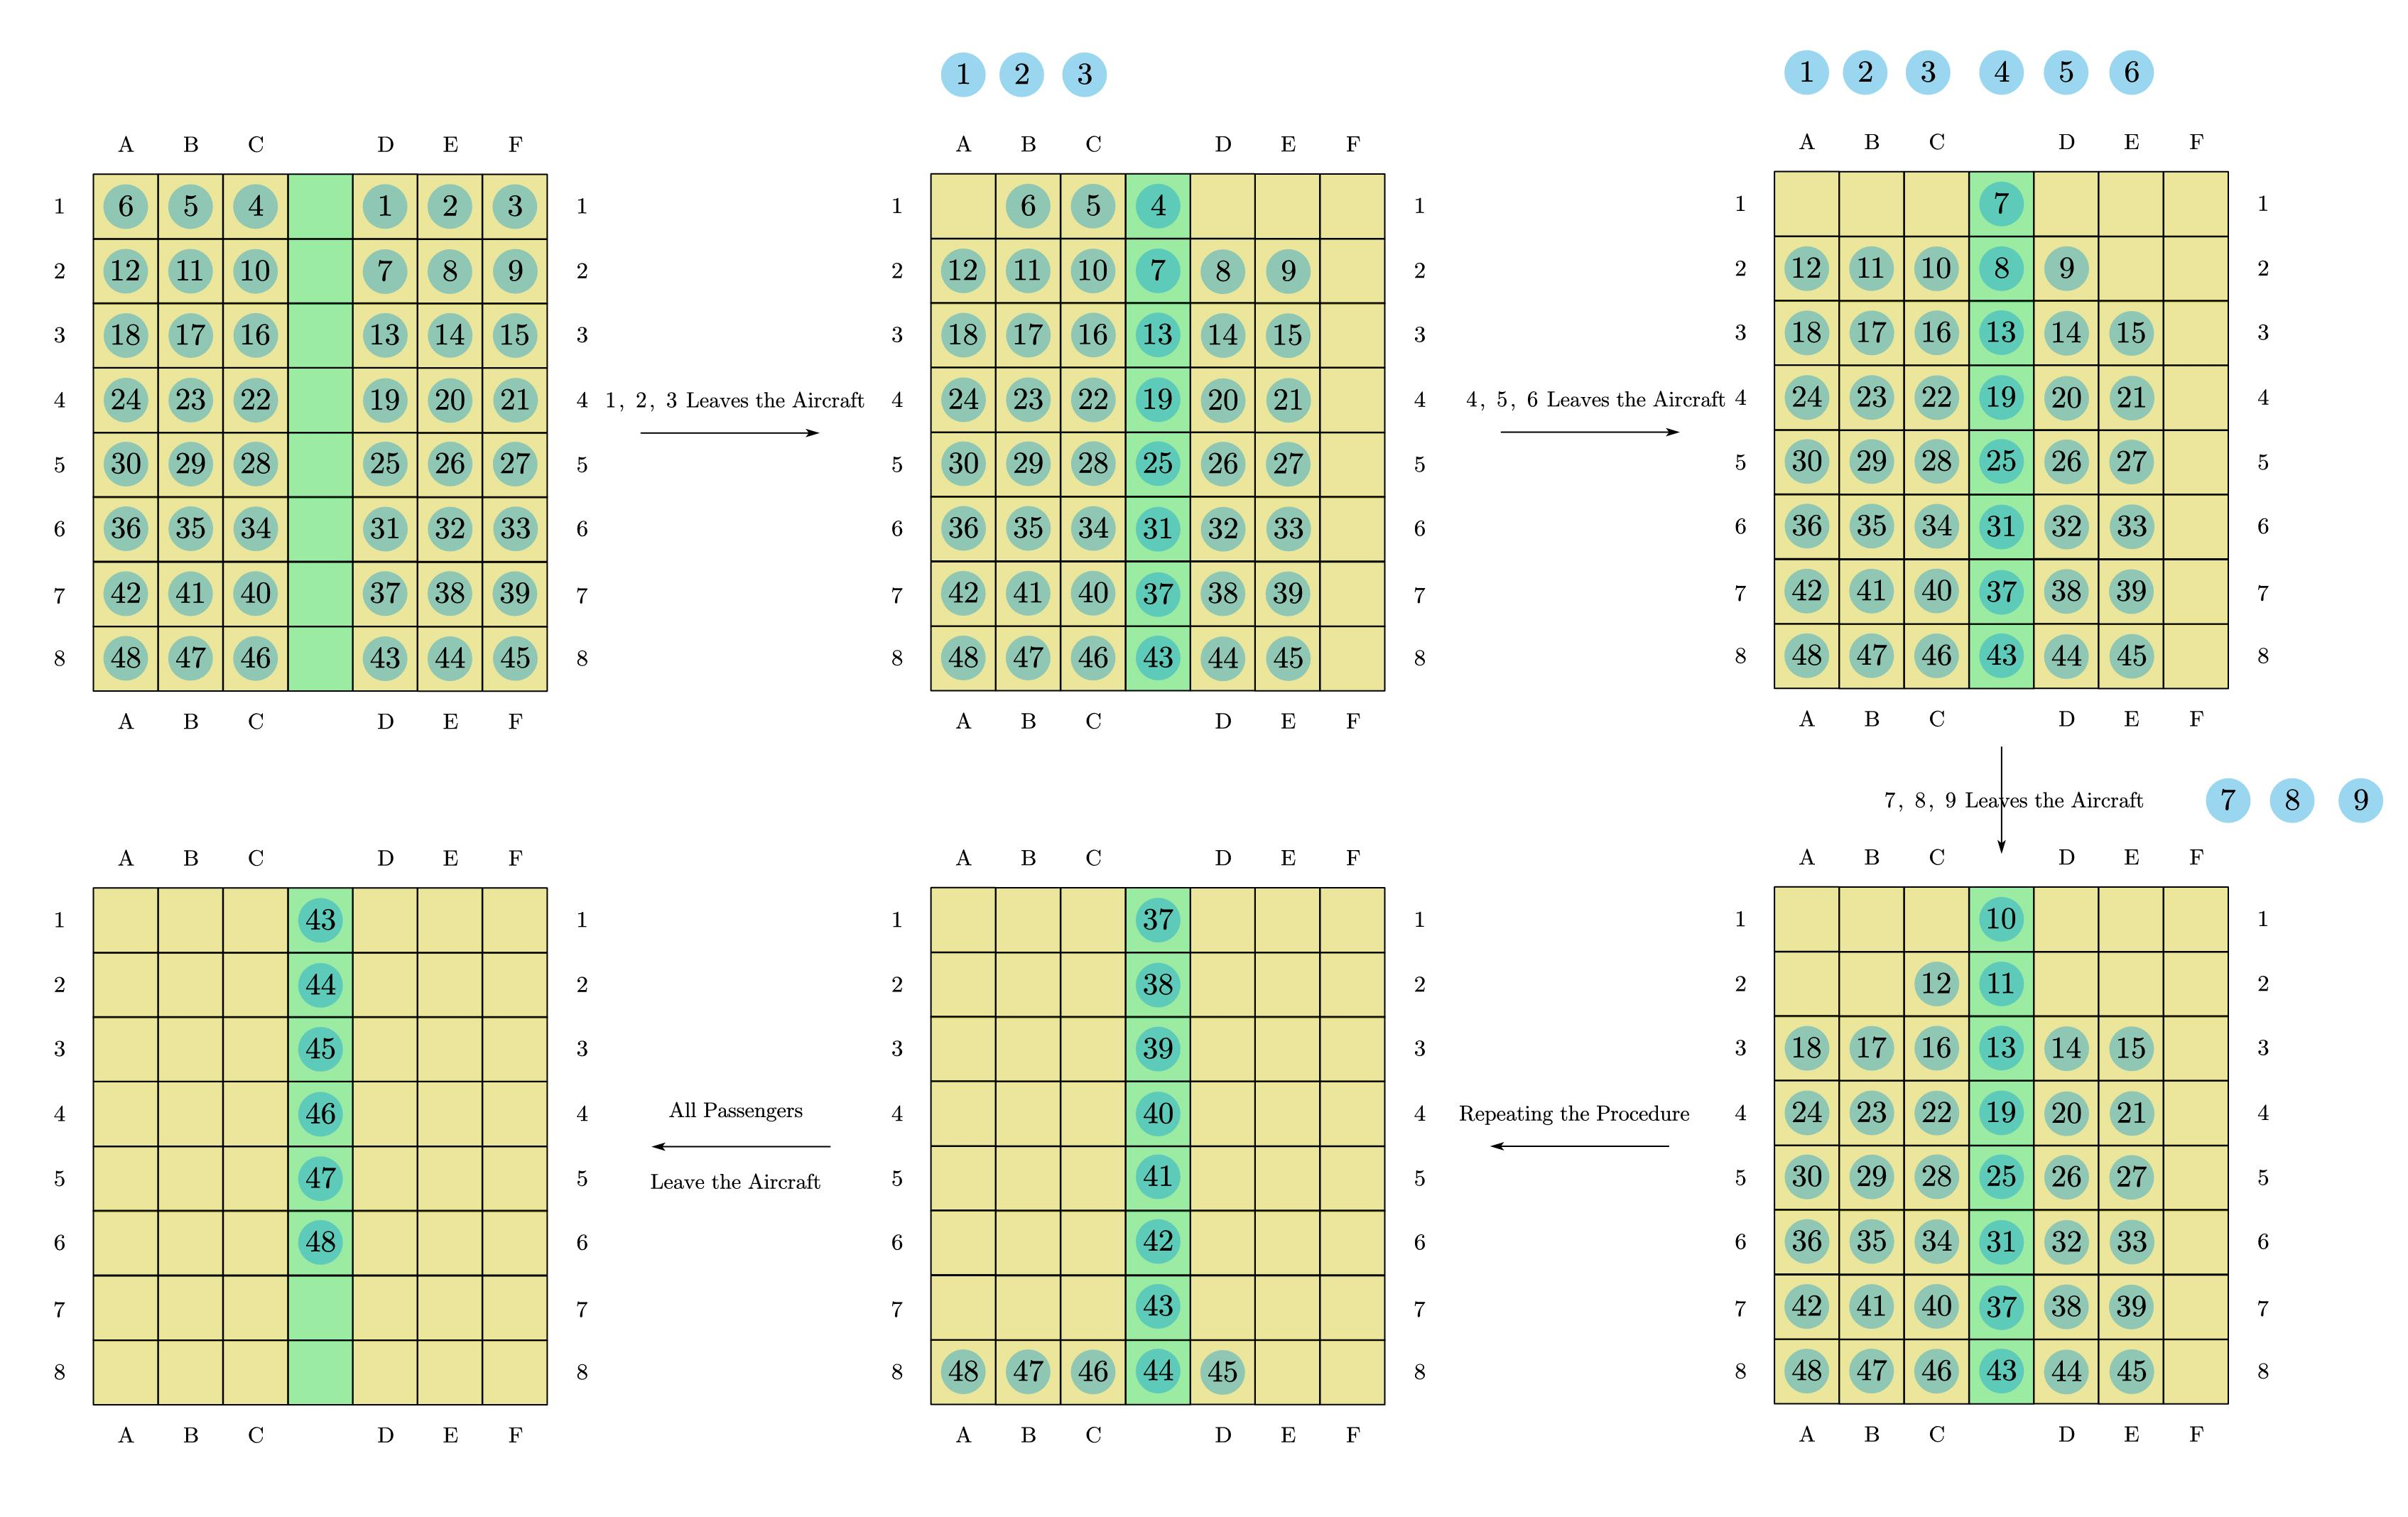
\includegraphics[width=15cm]{disembarking.jpg}

		\small \textit{Fig. best disembarking strategy}
	\end{center}

	Substitutions into the queuing model suggests that the time for a passenger to travel from the back to the front is 2199 time steps. After adding it to the time used to bring his luggage, we can find that the total disembarking time of our strategy is \textbf{12 minutes and 18 seconds}, which is surprising but also reasonable since most of the time spent on retrieving luggage is saved while others are queuing.

	\section{Model B: Reoptimizing the strategy with passenger satisfaction}
	\subsection{Model Overview}
	In model A, we've found the pattern of the optimal model. However, it's also crucial to notice the fact that in this model, passengers in the same row are highly separated. This would, as a result, greatly increase the dissatisfaction among families where parents should have been placed adjacent to their children in the queue. Therefore, in \defword{Model B}, we'll comprehensively consider passengers' satisfaction and therefore yield the most \textit{user-friendly} boarding strategy.
	\subsection{Notation}
	\begin{center}
	\begin{tabular}{|l|l|}
		\hline
		$\alpha_\text{satisfy}(A)$&satisfactory index of passenger $A$\\
		\hline
		$\alpha$&satisfactory index of a whole plan\\
		\hline
		$k_1$, $k_2$, $k_3$&constanrts describing the weight of each factor\\
		\hline
		$D_i$&variance of the boarding time of the passenger whose seat is in the $i^\text{th}$ row\\
		\hline
		\(\xi\left(A\right)\) & the total time passenger A needs to offer his/her seat\\
		\hline
	\end{tabular}
	\end{center}
	\subsection{How Satisfied the Passenger is?}
	In this part, we mainly dicuss which methods can best satsify the passengers.

	\begin{itemize}
		\item \defword{Queuing}: The longer a customer stays in a queue, the less satisfied he is.
		\item \defword{Offering one's seat}: The passenger who sits near the aisle will be especially dissatisfied when people who sit near the window ask for his offering seat.
		\item \defword{Walking}: With luggages with him,, walking a long distance in the plane will make the passengers impatient. The more he walks, the worse his mood will get.
	\end{itemize}
	To make our result more precise, we define a series of constants ($k_1$, $k_2$ and $k_3$) to determine the factors' weight. To standardize our calculations, we take $k_1$ as the criteria number 1. As mentioned above, passengers will get angry when they are offering their seat and this will have a dramatic effect on the passenger's satisfactory degree, and long distance of walking will also have more effect on a person's mood. By looking into the order of magnitude and past experience, we set \(k_2\) as \(250\) and \(k_3\) as \(10\).
	Together we find out the definition of satisfactory factory of a certain passenger, which is:

	$$\alpha_\text{satisfy}(A)=k_1\cdot \tau_j(A)+k_2\cdot\xi\left(A\right)+k_3\cdot D_i$$
	The re-weighed indexes and the correspondent \(\alpha_{\mathrm{satisfy}}\,\)s are shown below.
	\begin{center}
		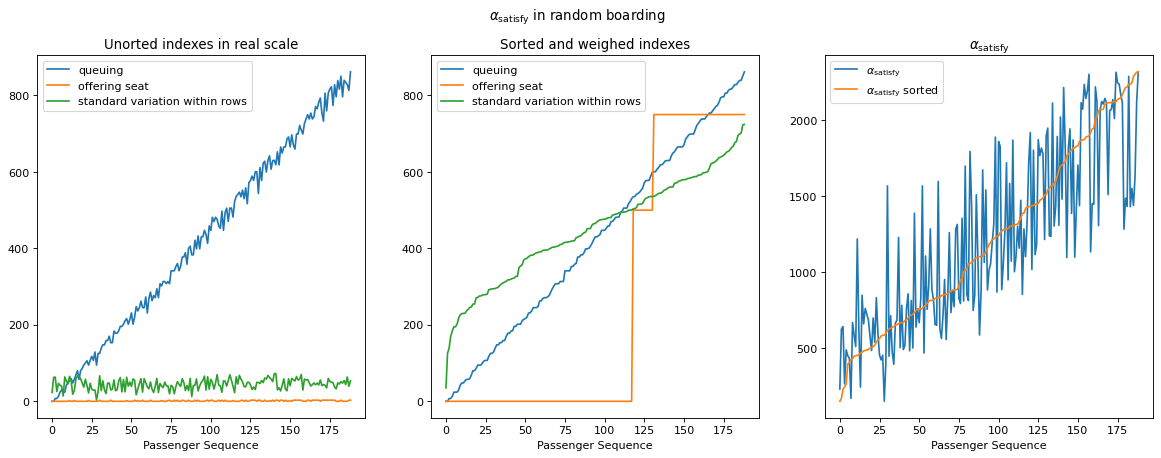
\includegraphics[width = 17cm]{random satis.png}

		\small\textit{Fig. \(\alpha_{\mathrm{satisfy}}\) in random boarding}
	\end{center}
	To sum up, we can get the satisfactory index of a whole plan. The bigger $\alpha$ is, the less satisfied the passengers are and the less possible the plan can be applied to daily life.
	$$\alpha=\dfrac{\sum\limits_{A\in P} \alpha_\text{satisfy}(A)}{N}$$
	In this case, \(\alpha\) equals \(1222.25\) in random boarding.

	\subsection{Analysis of Different Ways of Boarding}
	In this part, we will introduce some common ways of boarding and find out their effiencies based on the $\Gamma$ and $\alpha_\text{satisfy}$ of it. The picture below shows the plane we use to assess the boarding process.

	\subsubsection{Introduction of Conventional Boarding methods}
	The first method is based on row numbers. People enter the plane according to their row number. The plane is divided into several crosswide sections.or example, in one plan, a passenger with a smaller row number can be seated earlier and in other plane, he will enter later. We conclude these types as "front to back" and "back to front".

	The second method is to board on plane according to their seat positions. The plane is divided into lengthways sections in this strategy. This time, passengers whose seats are A or F may enter the plane first to minimize the time wasted in offering seats.

	The third method, window-middle-aisle boarding, lets passengers board according to an inner-to-outer sequence. We subdivide this method into another three forms: random, front to back, and back to front, which respectively indicate the boarding sequence in each \textit{window, middle or aisle} section. This plan can effectively reduce the total disembarking time as people no lobger need to worry about offering their seat to others. Although it may make people unsatisfied (the reason will be introduced in the next model), it does save time.

	Another way of boarding is letting the passengers get onboard in an unstructured way, which means that the boarding order is random. The picture below shows the whole process of this boarding method.

	The four pictures below can effectively explain the methods.

	\begin{center}
		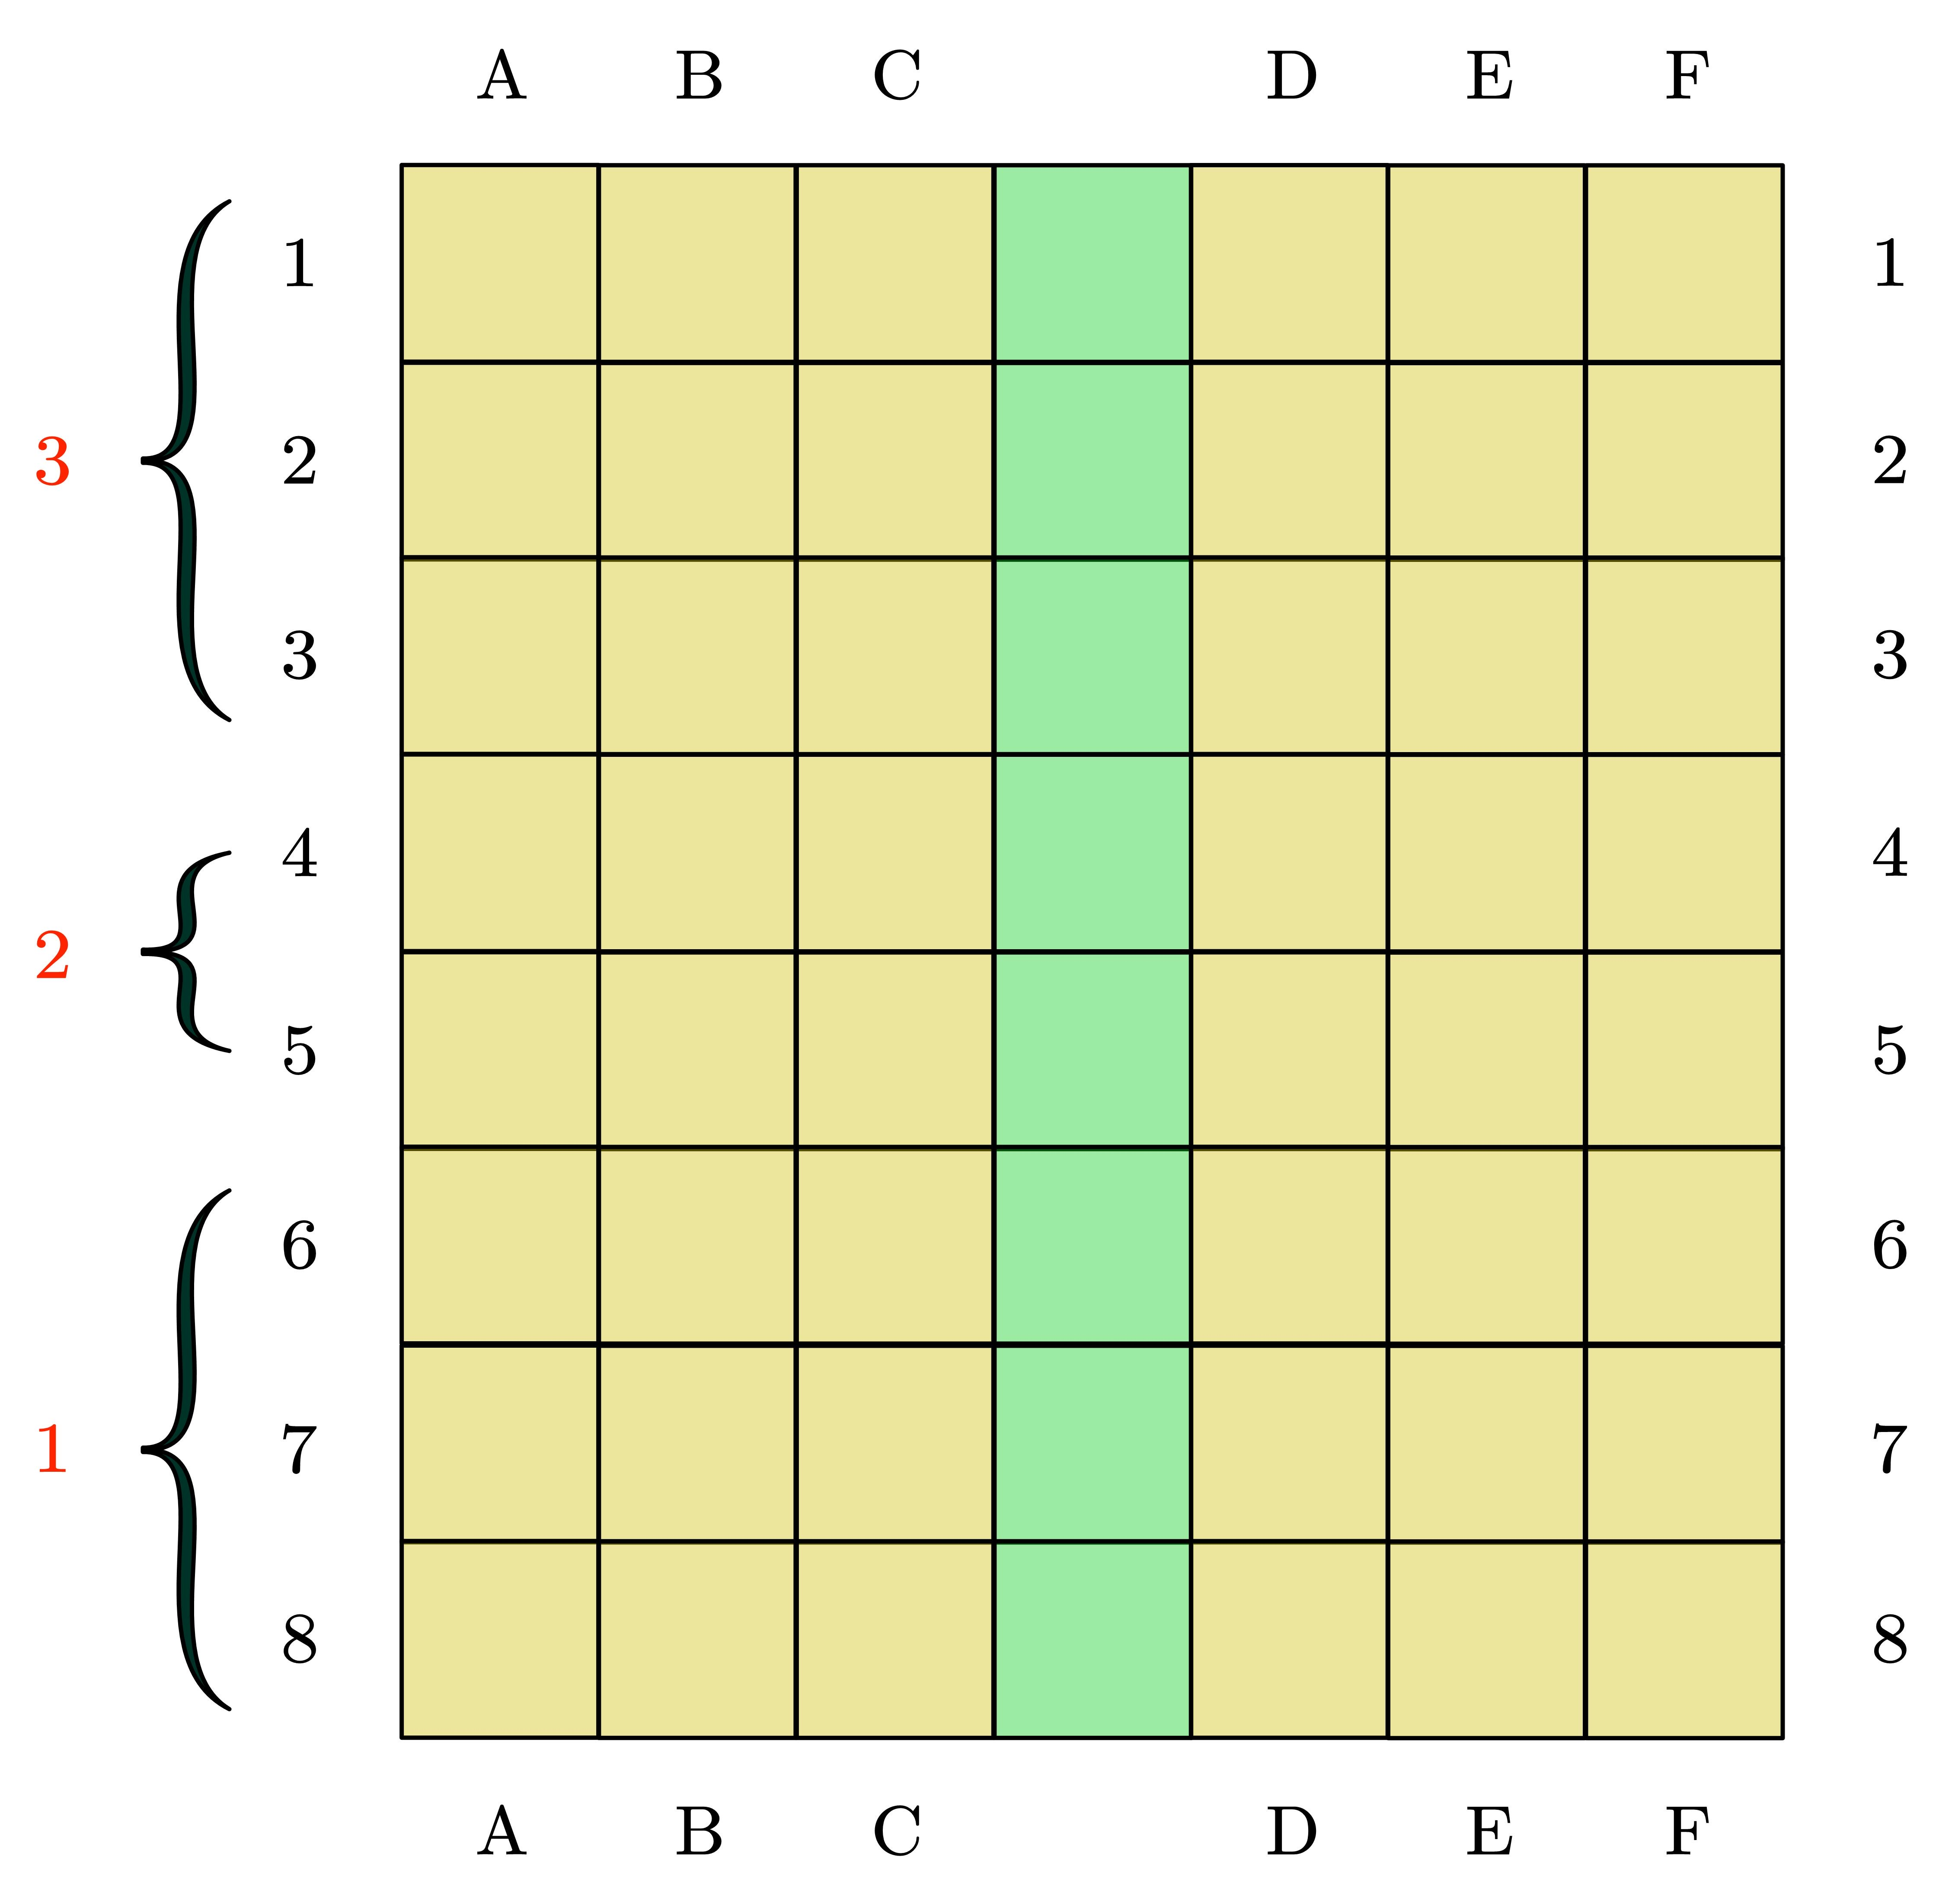
\includegraphics[height=3.7cm]{planerow1.jpg}
		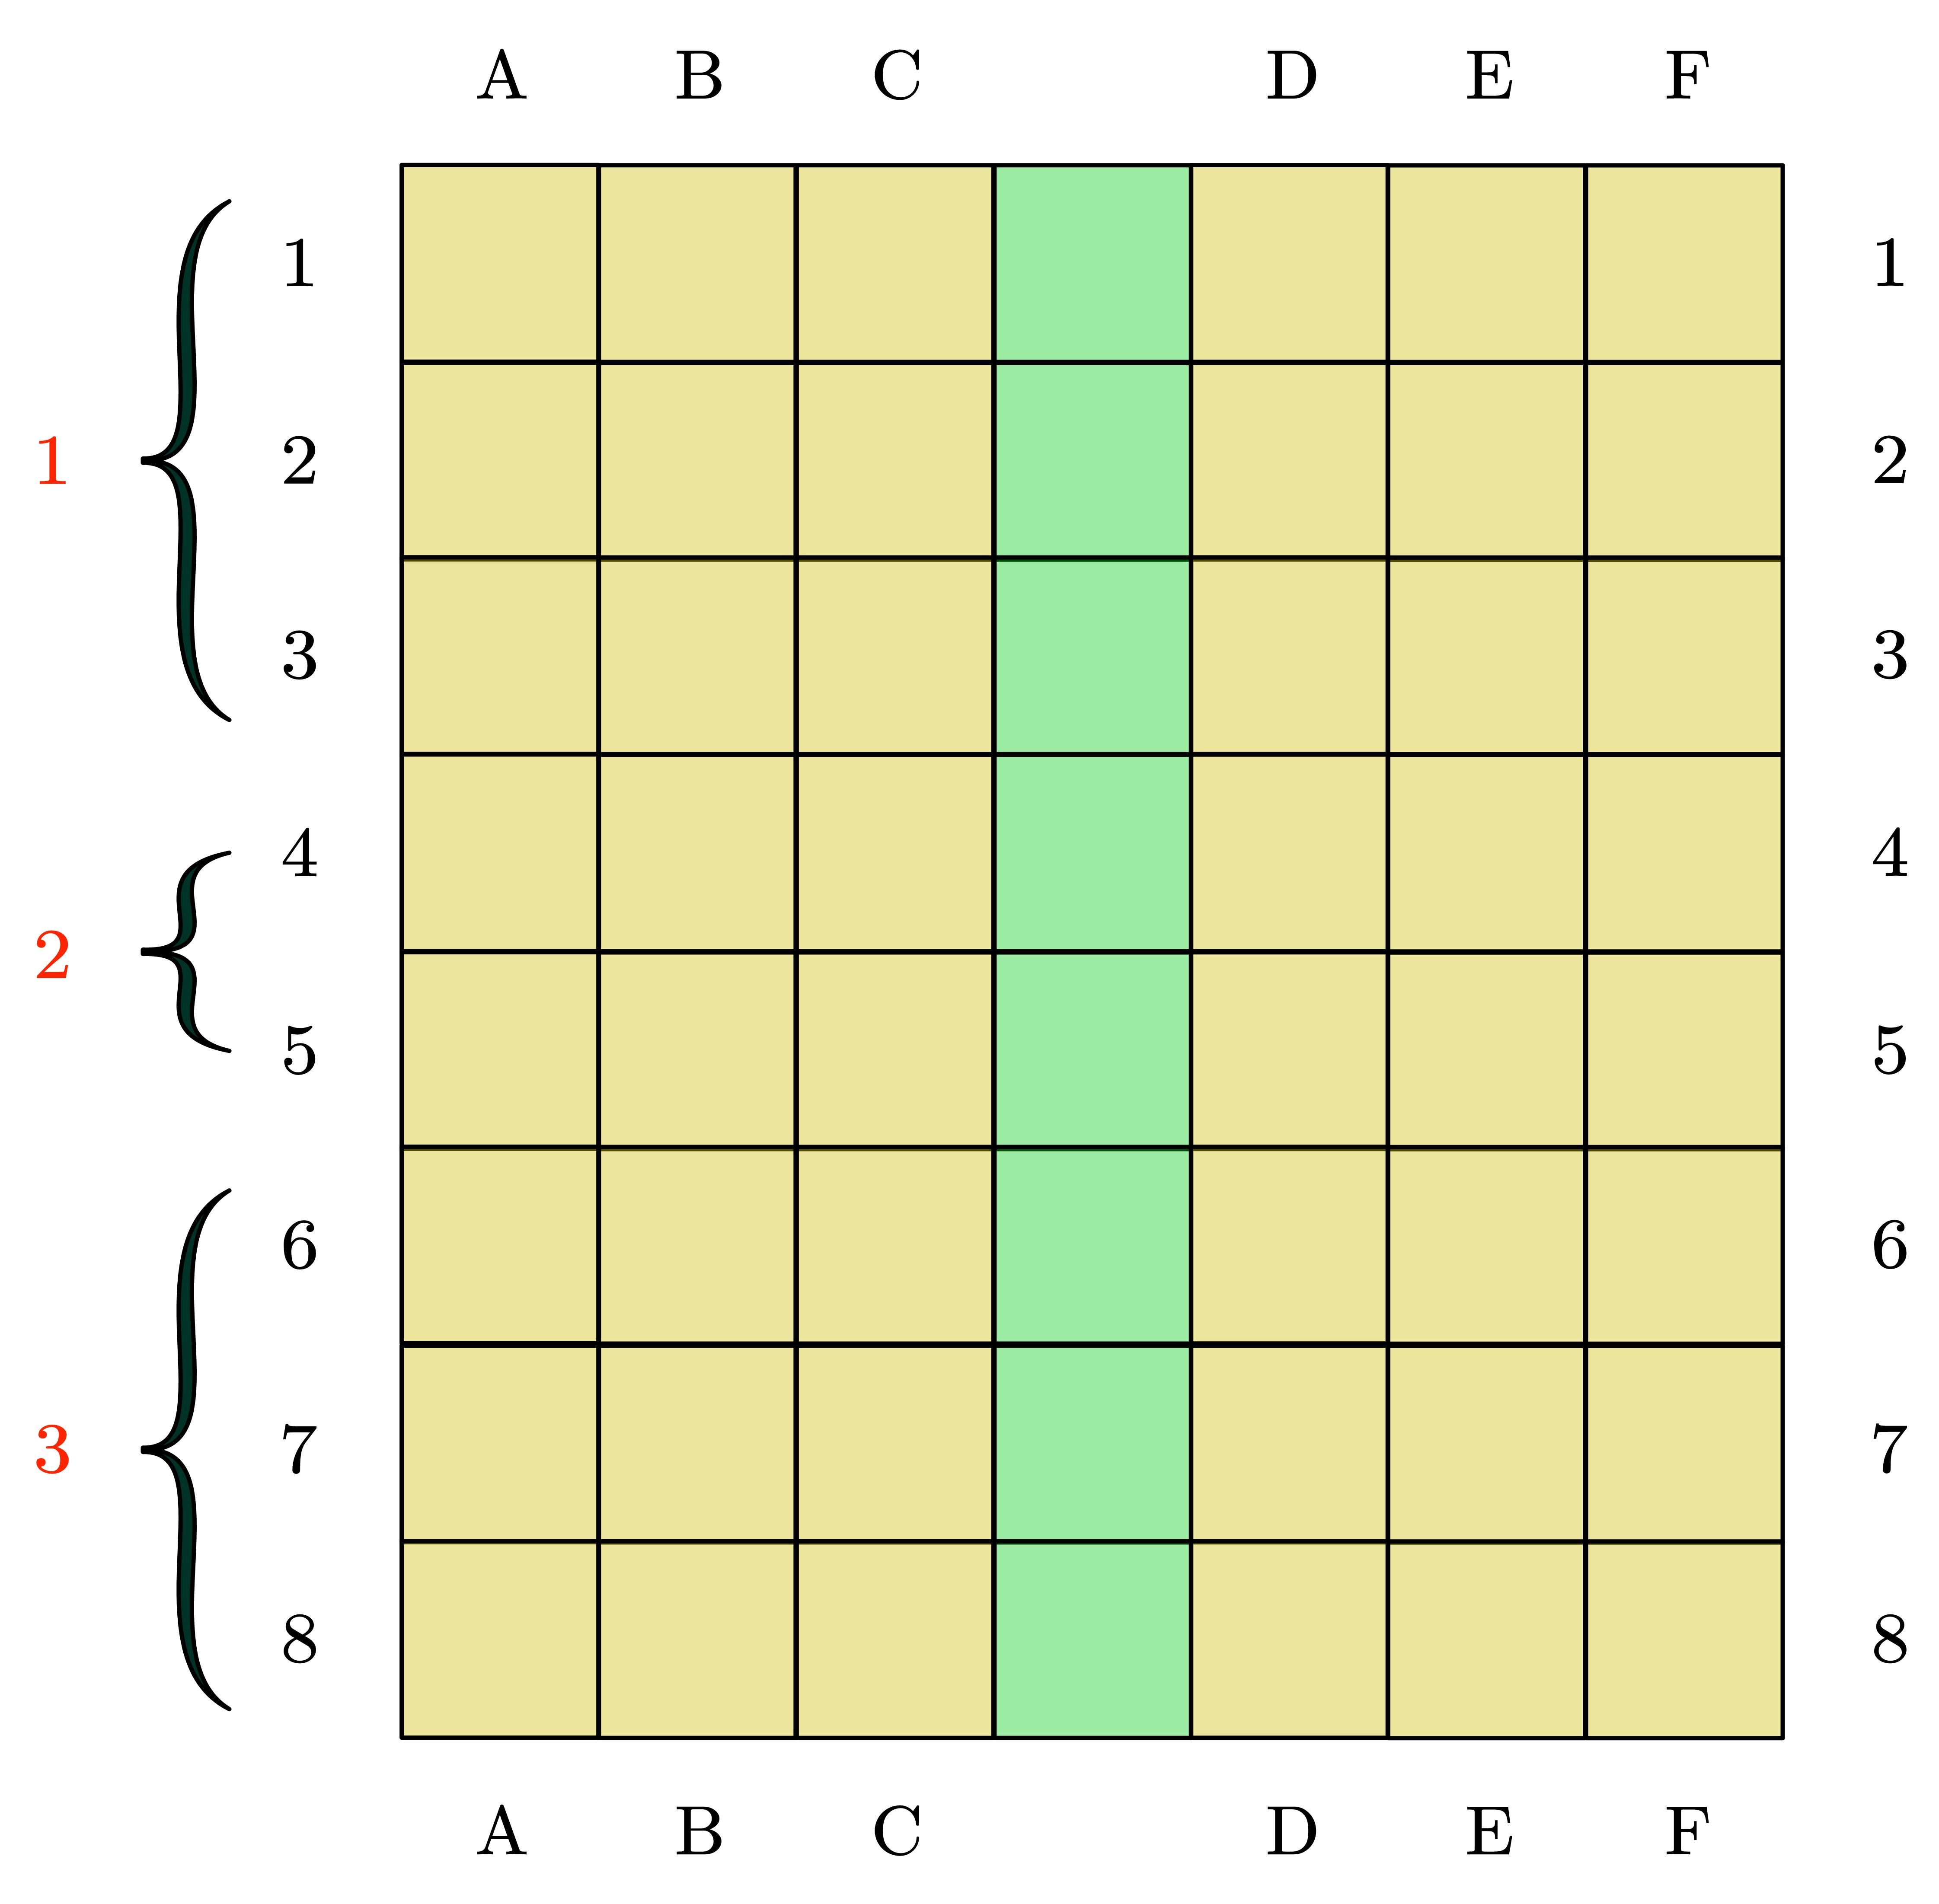
\includegraphics[height=3.7cm]{planerow2.jpg}
		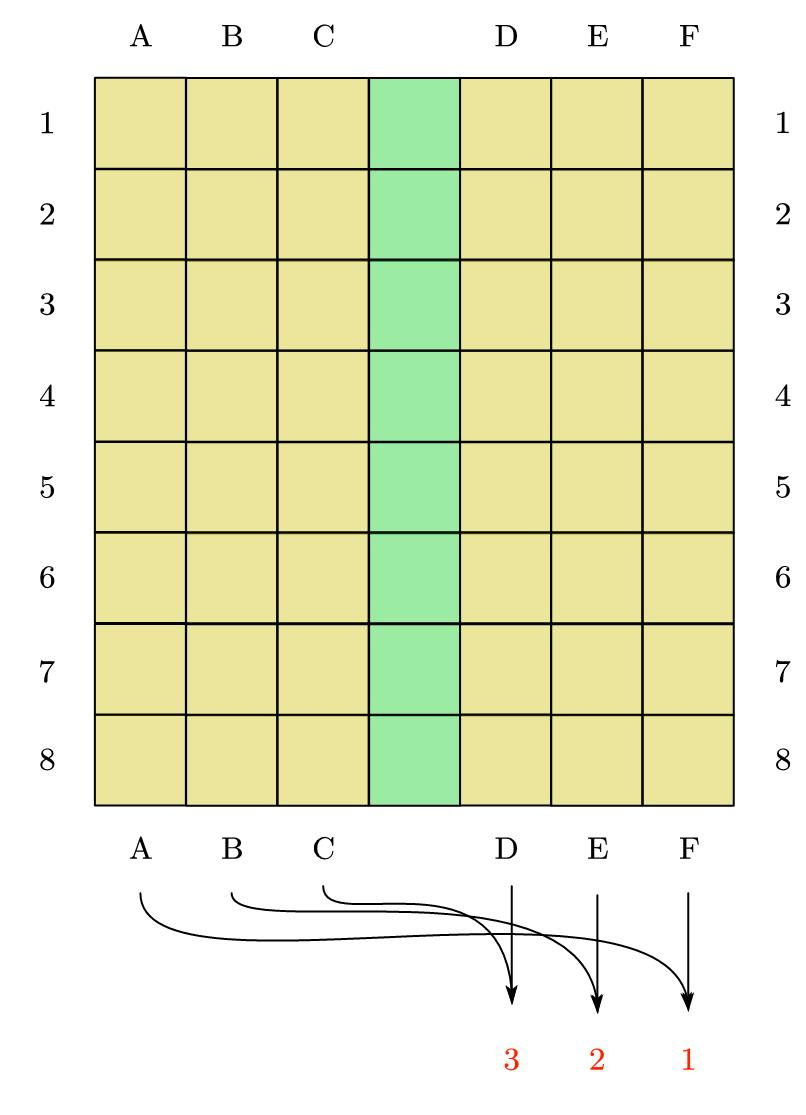
\includegraphics[height=3.7cm]{wdmd.jpg}
		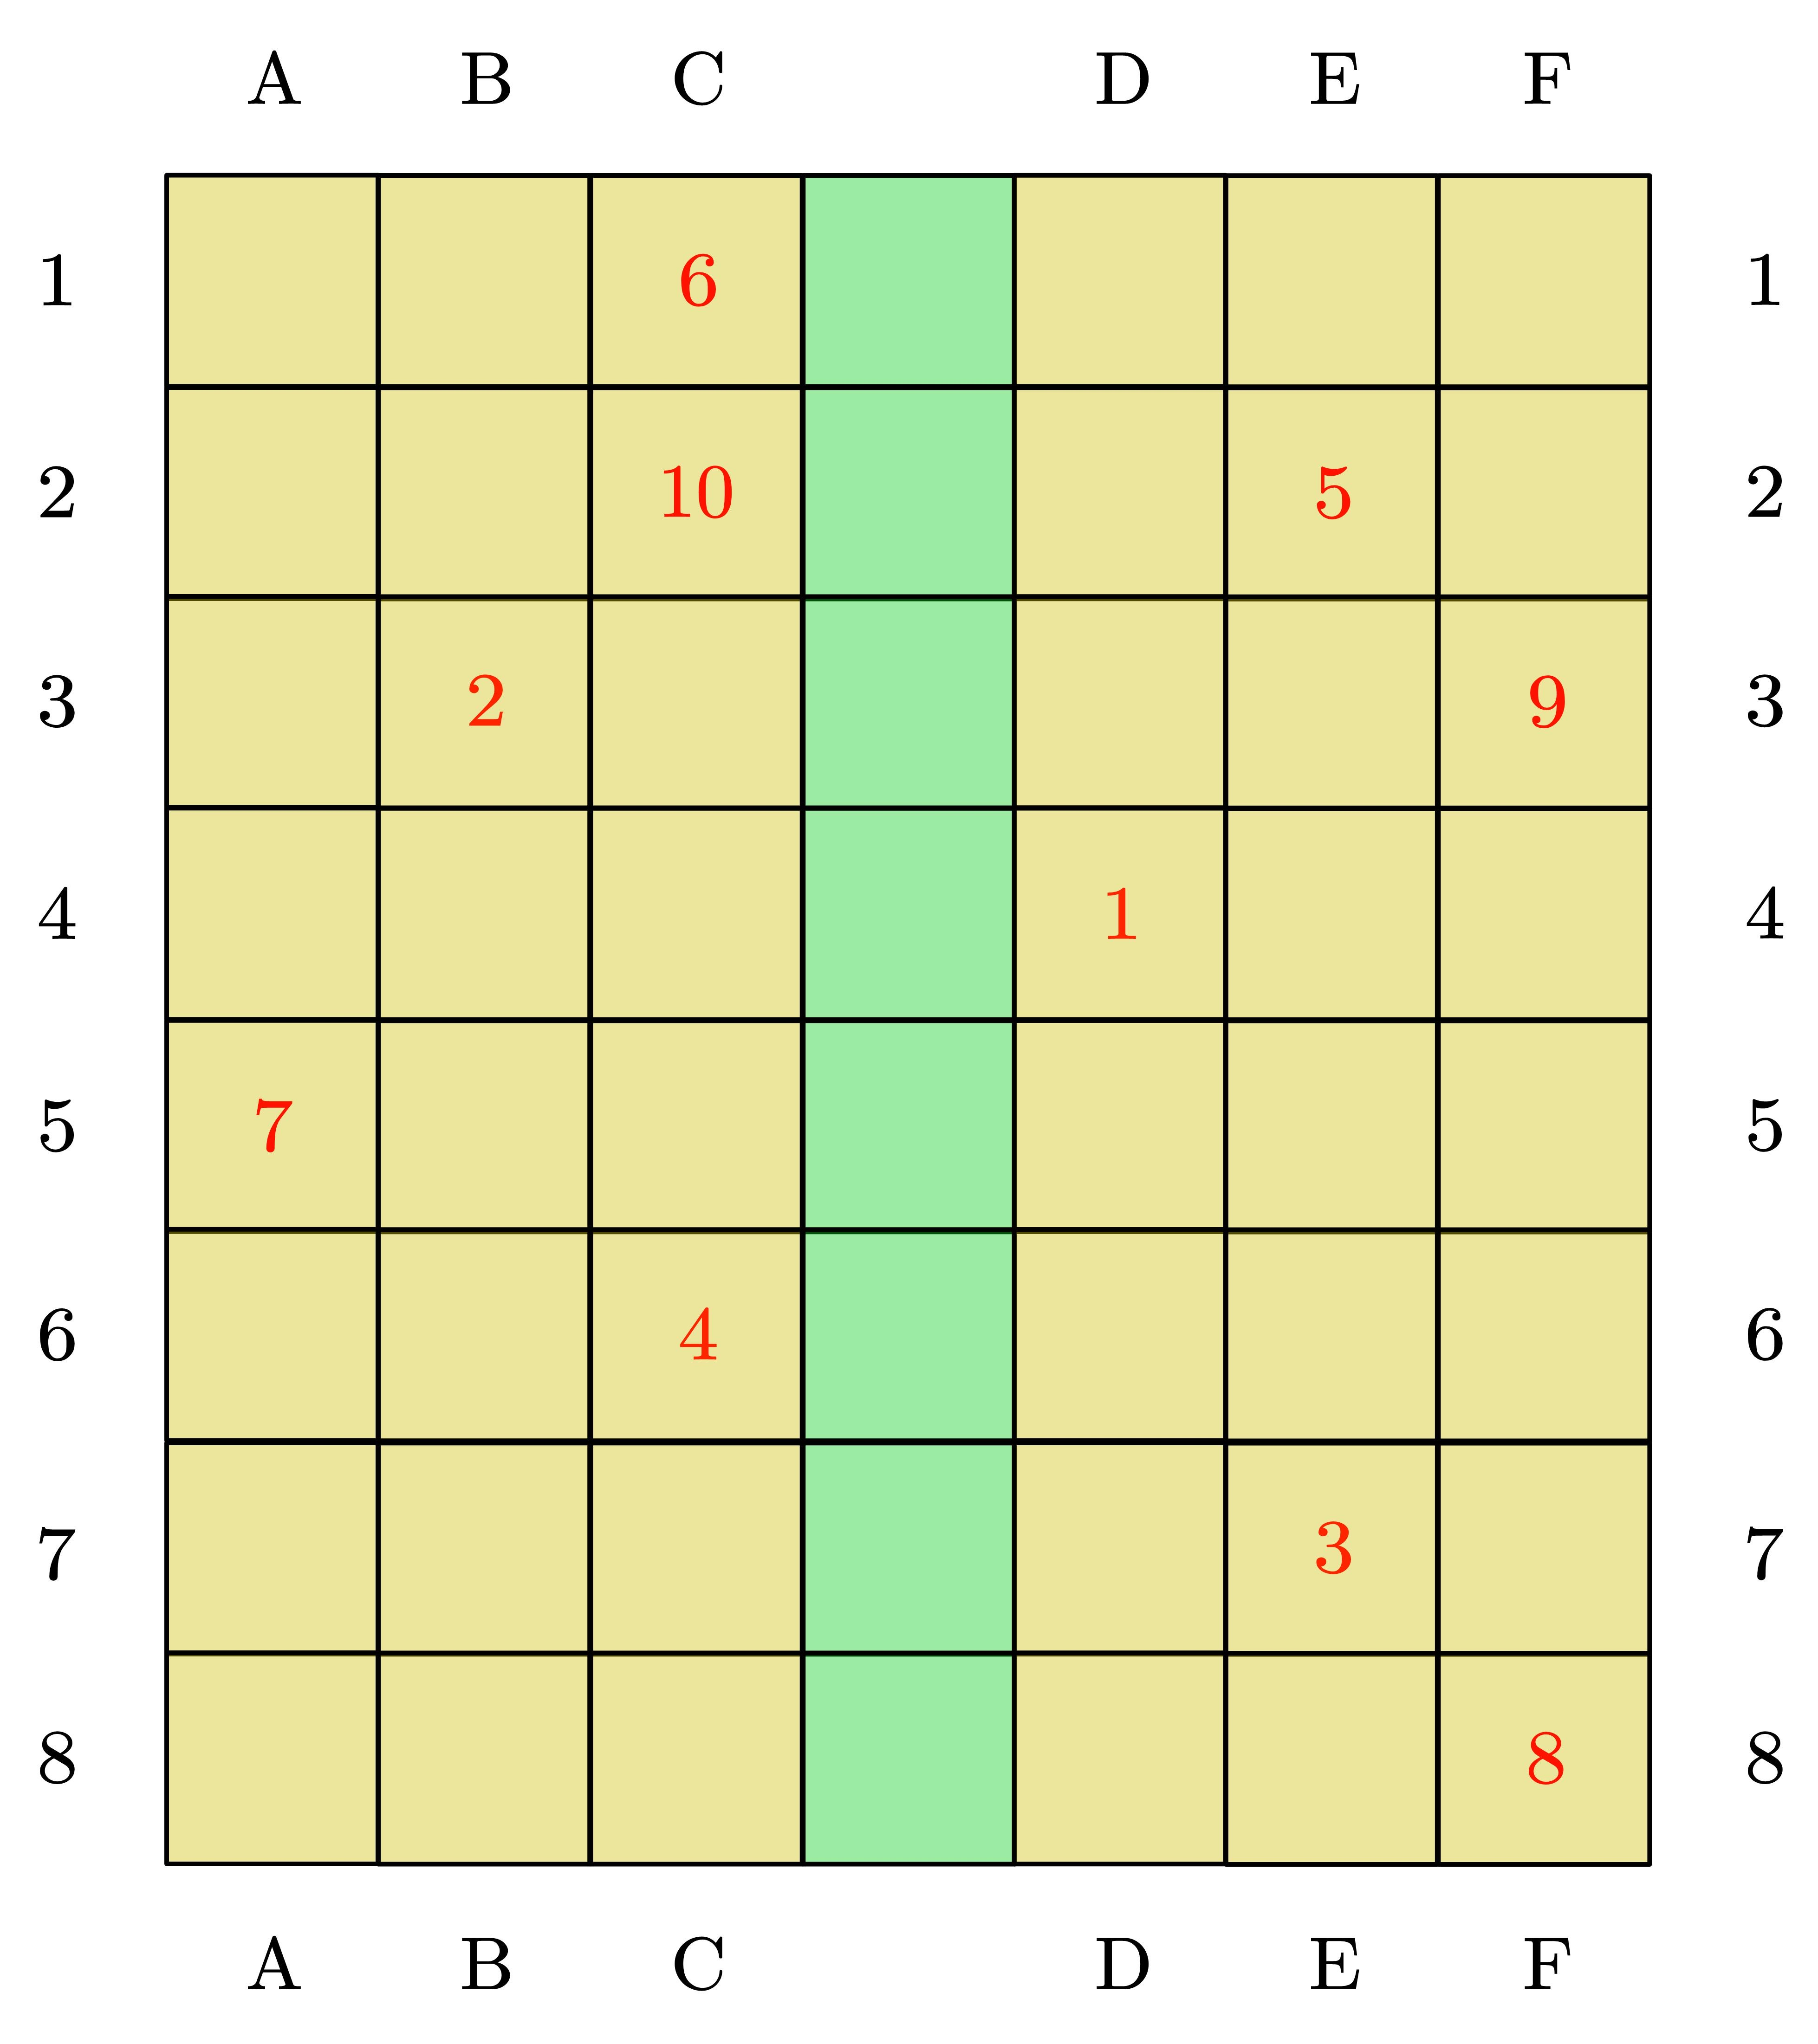
\includegraphics[height=3.7cm]{planerandom.jpg}

		\small \textit{Fig. Left \(\to\) Right: Back-to-front, Front-to-back, window-middle-aisle, and random boarding}
	\end{center}
	\subsubsection{Yielding Results}

	By substituting the data of the strategy back into our previous model, we can draw a table to compare $\Gamma$ and $\alpha_\text{satisfy}$.

	\begin{center}
	\begin{tabular}{||l|l|l||}
		\hline
		Boarding type&Time steps required&$\alpha_\text{satisfy}$\\
		\hline
		From front to back&5029&938.82\\
		From back to front&4092&854.01\\
		Random Window middle aisle&4347&1207.81\\
		Back-to-front Window middle aisle&4120&1482.14\\
		Front-to-back Window middle aisle&4398&1501.17\\
		Random Boarding&4409&1222.25\\
		\hline
	\end{tabular}
	\end{center}
	From this we can find that, boarding from front to back needs the maximum time, which means that it may not be so reasonable when applied to daily life. Boarding from back to front, on the other hand, is the most  efficient time. However, its easy to find that the difference between the three latter methods is not significant, which we will explore further in \defword{Sensitivity Analysis}.

	Apart from the common ways used by air executives introduced above, we also figure out some plans of our own and proposed by others. They all share one feature in common: \textbf{fast total boarding speed} and \textbf{high parallelity}.
	\begin{itemize}
		\item The first plan introduced is the Steffen Perfect\cite{steffen}. In this mode,  passengers will board the plane from the inner seat to the outer seat, from the rear to the front and in separate rows. Because the passengers sitting on the back and inside board first, there will be no queuing caused by the luggage of the front passengers and the situation that the outer passengers give up their seats for the inner passengers, which effectively reduces the waste of time caused by congestion and seat giving. At the same time, when boarding, passengers who put their luggage generally need to occupy the aisle next to two rows of seats. Therefore, it can be proved that sitting in separate rows is a seating method with the highest parallel efficiency, which can allow the most passengers to sit in parallel. Taken together, this shows that Steffen Perfect is a great boarding strategy.

		\item Another optimal boarding strategy is to divide the plane into five parts (demonstrated in the picture below). This strategy combine all the strengths together: it can perfectly reduced the time of offering seats, queuing and raise the passenger's satisfactory index. However, this may also lead to some other problems.

		\begin{center}
			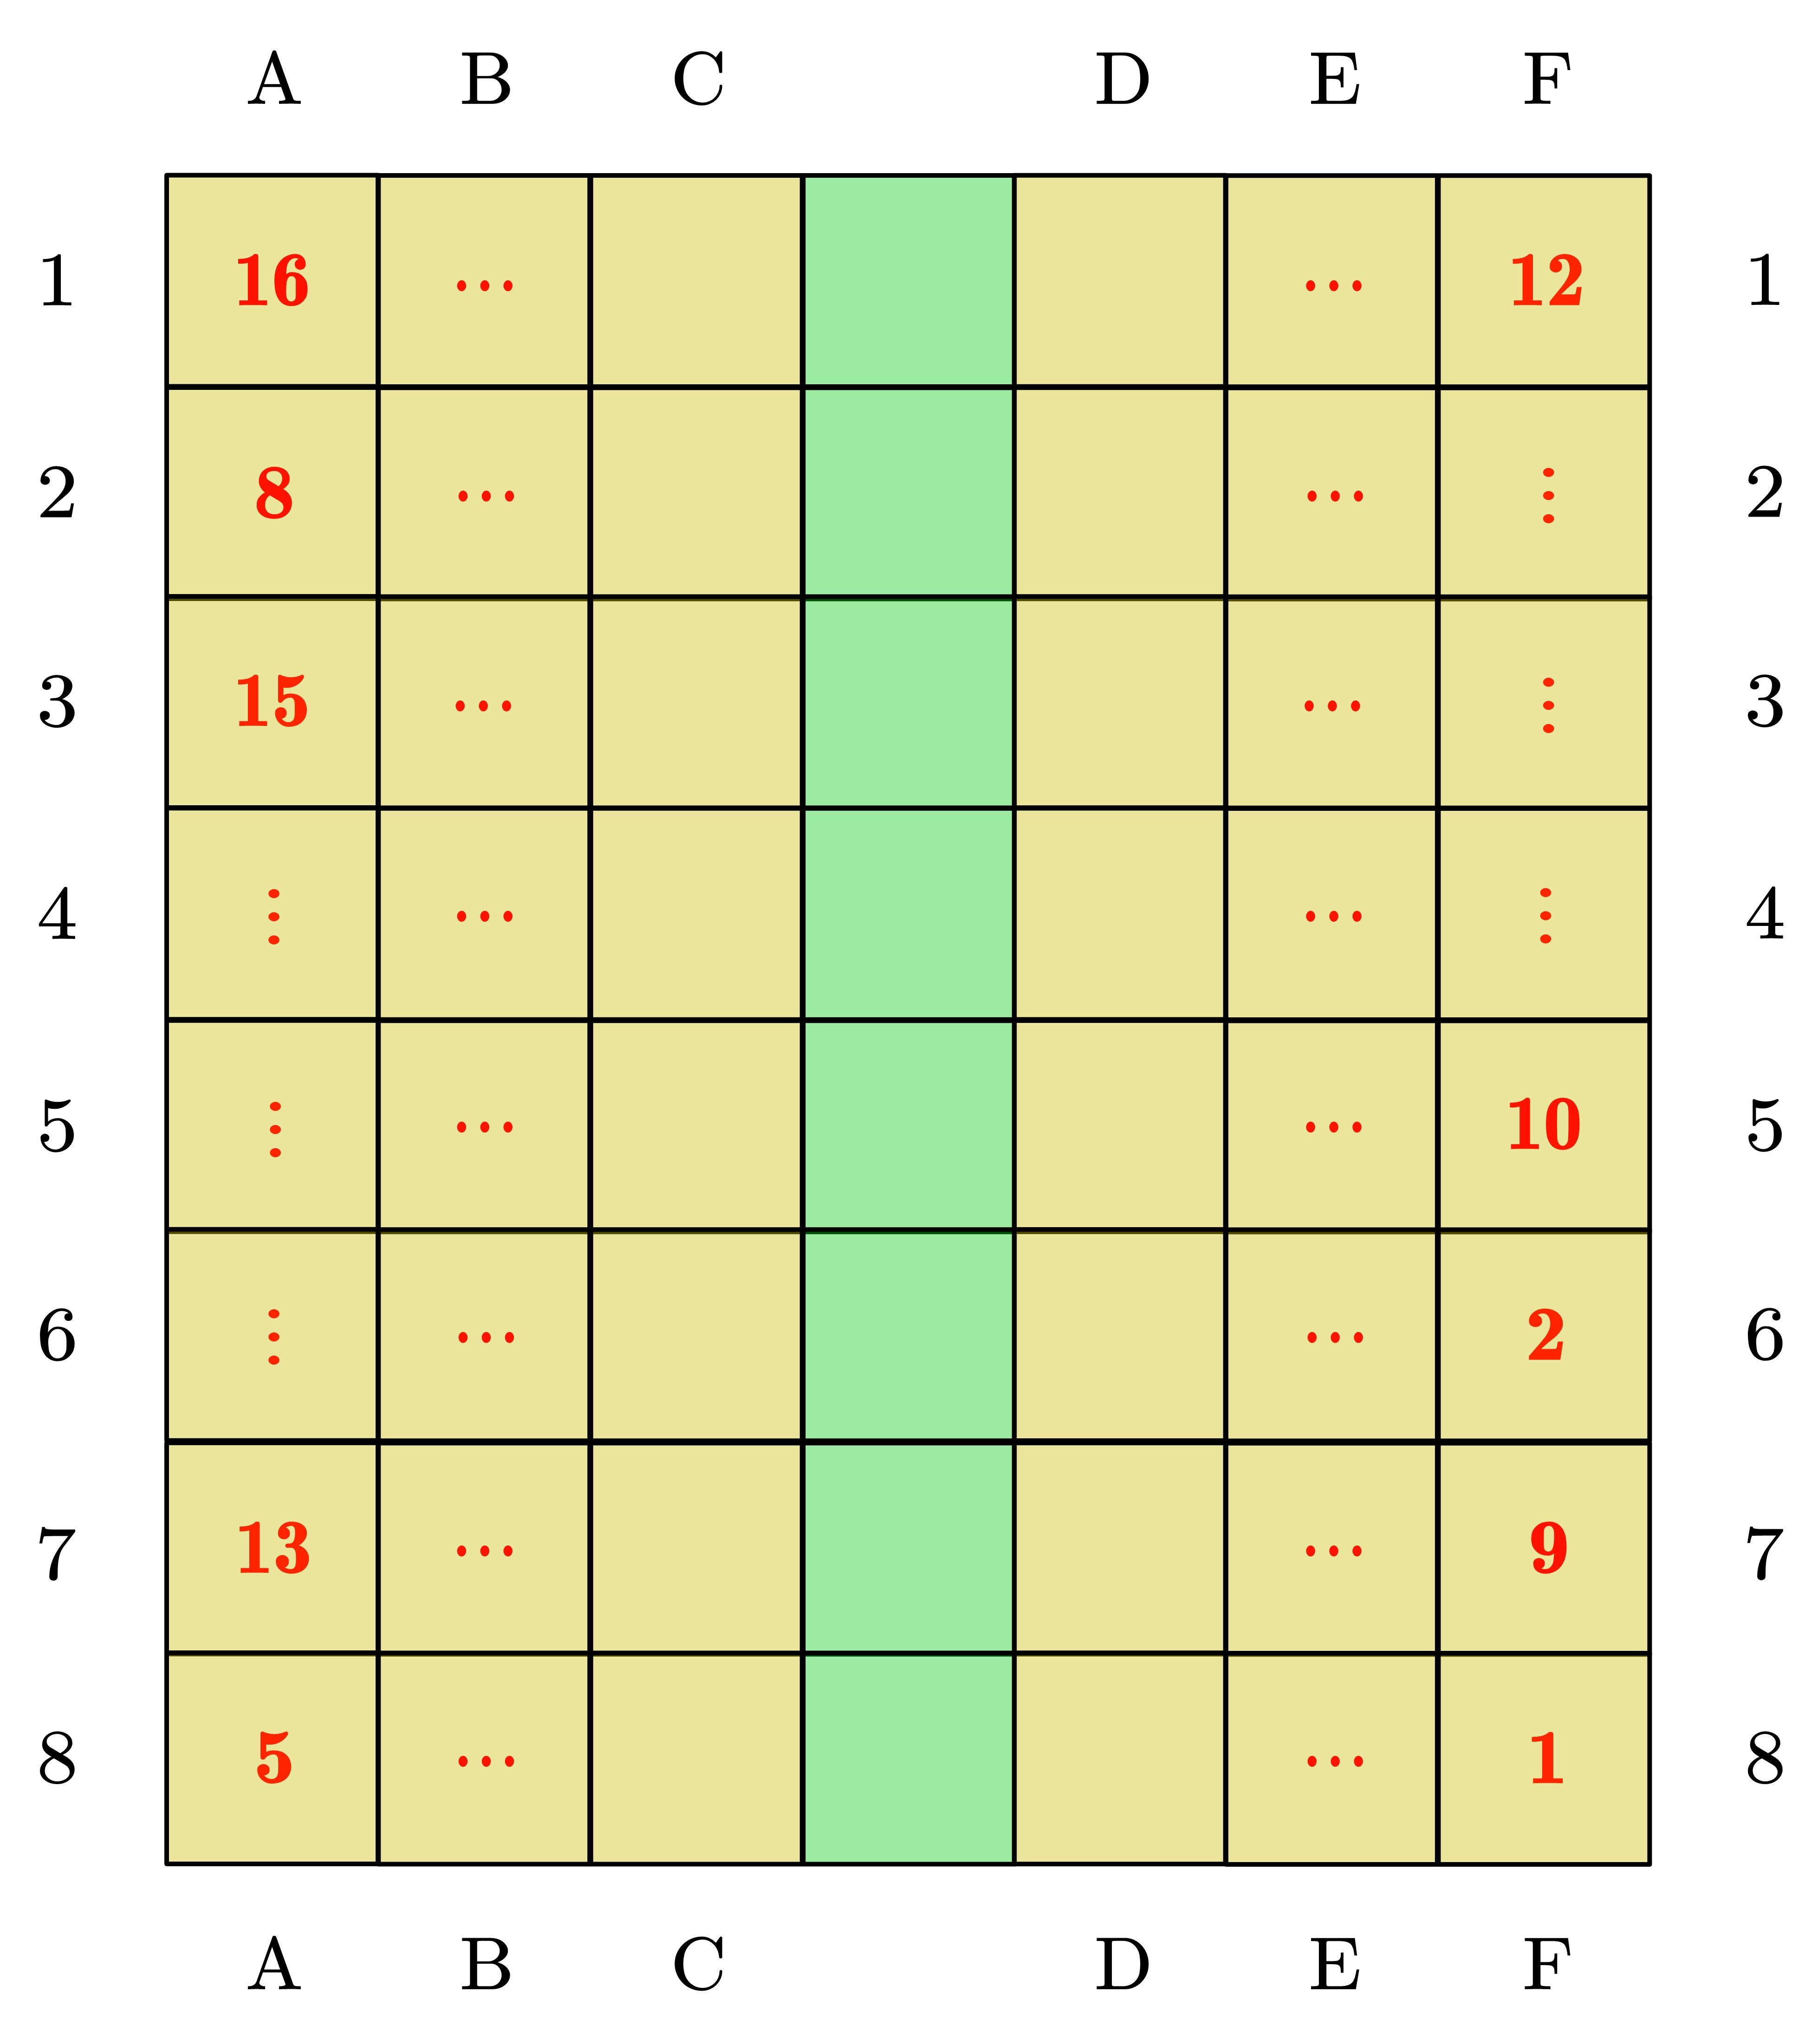
\includegraphics[height = 4.5cm]{stf_perfect.jpg}
			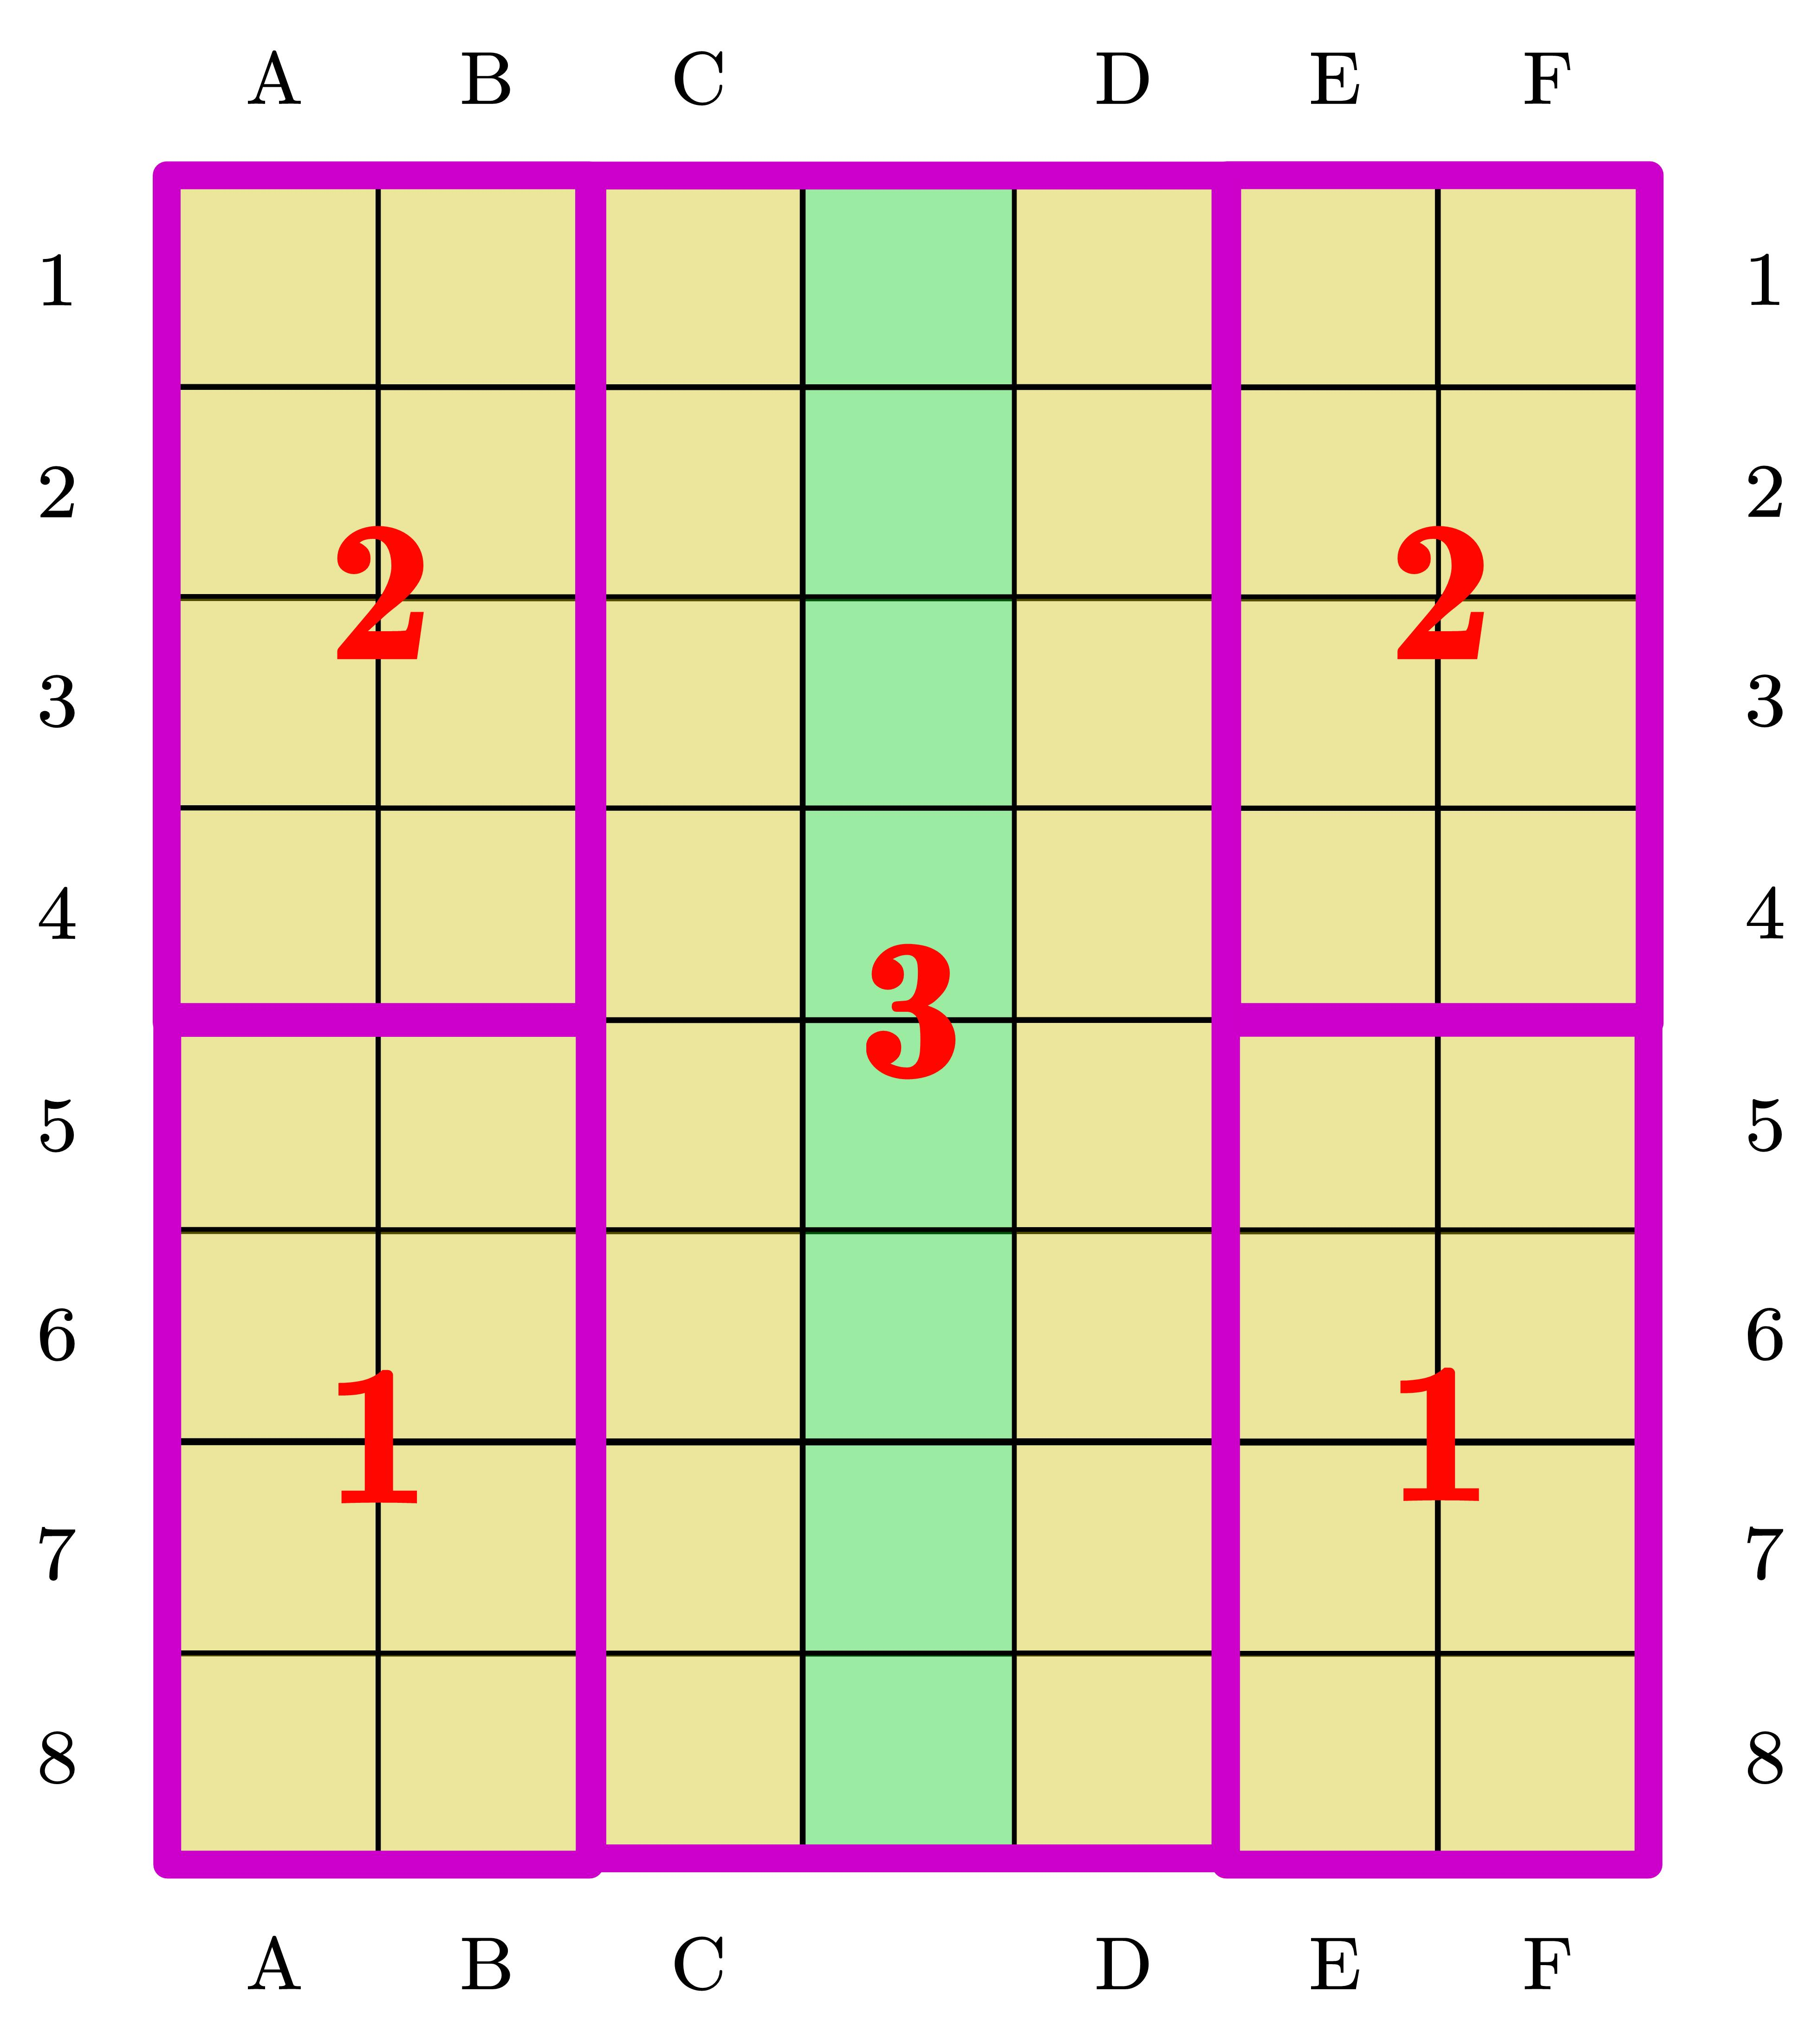
\includegraphics[height=4.5cm]{planeown.jpg}
			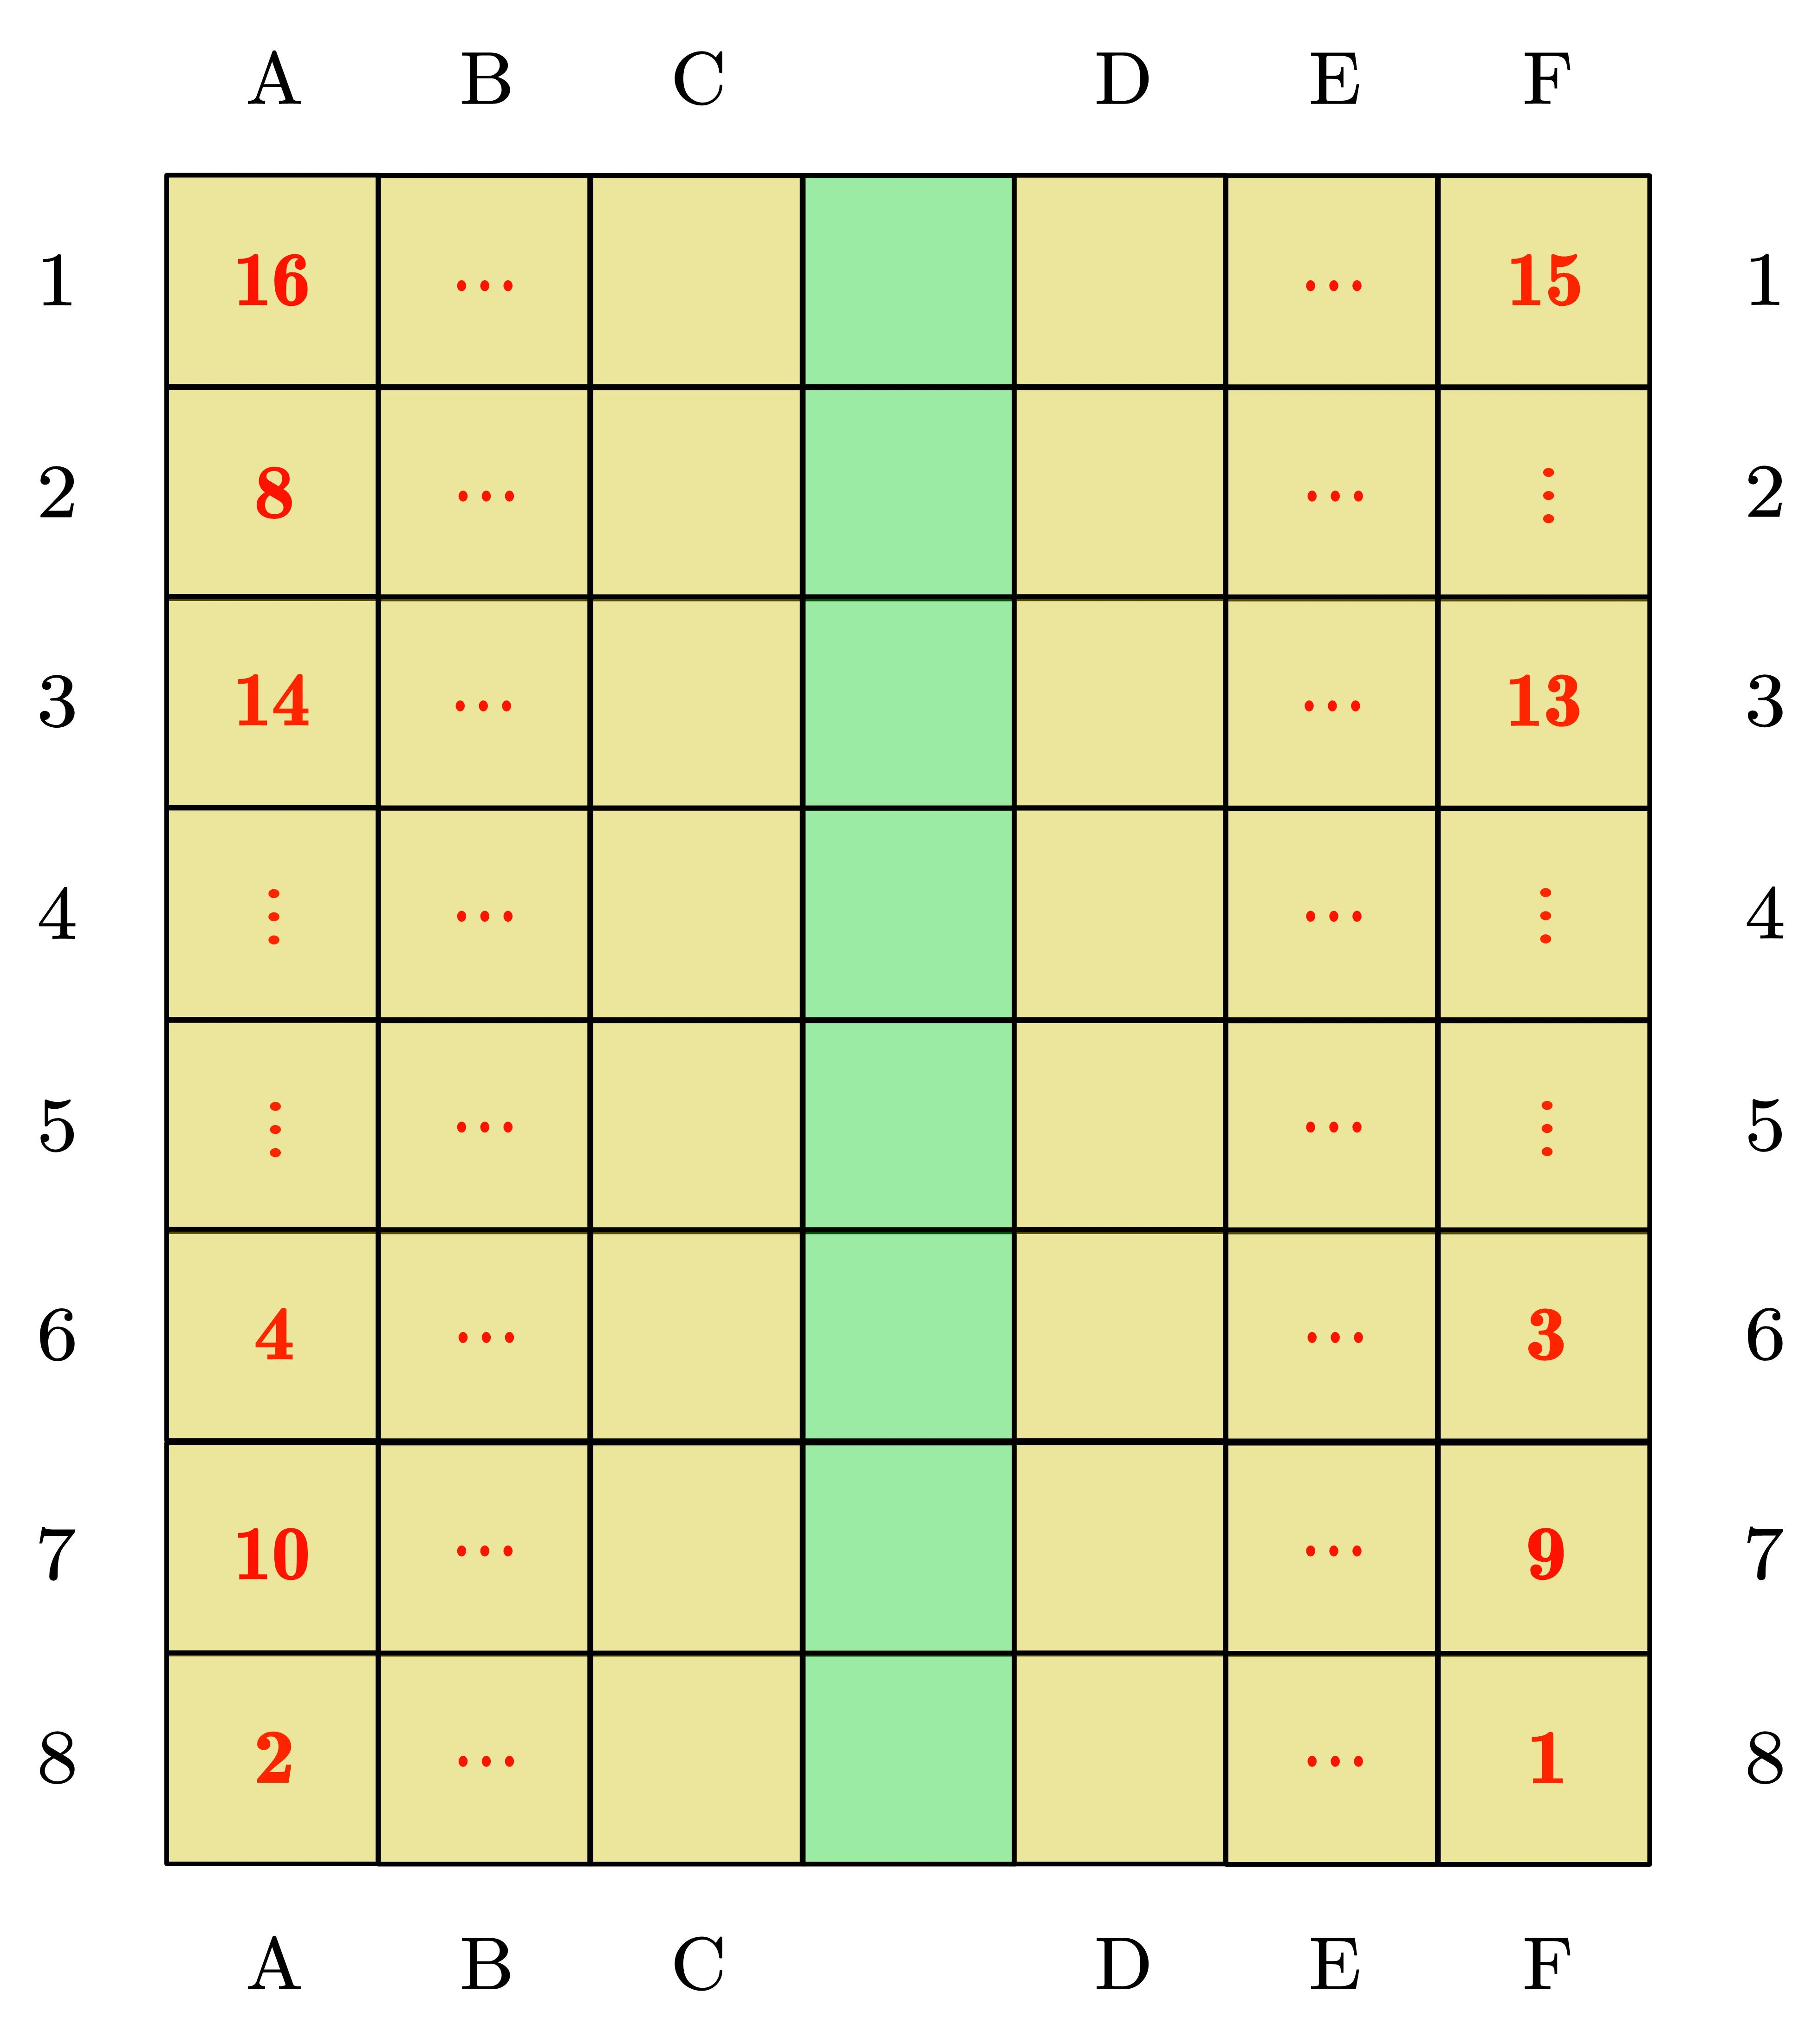
\includegraphics[height = 4.5cm]{stf_subperfect.jpg}

			\small\textit{Fig. Steffen Perfect, Boarding by section \& Steffen Sub-perfect}
		\end{center}

		\item The third plan, which is what our \textbf{optimization model} suggests, is what we name as \defword{Steffen Sub-perfect} due to its similarity to the \defword{Steffen Perfect} boarding method. However, the biggest difference is that the passengers in the same row would not board together. Instead, the passengers in the upper and downer part would alternately board. Because of the similarity, it is also an optimized strategy. In fact, according to computer simulation, it's even a bit faster than Steffen perfect.
	\end{itemize}
	Now we plot all the suggested methods below in one plot. It shows the relationship of total number of seated passengers with the time step \(t\).
	\begin{center}
		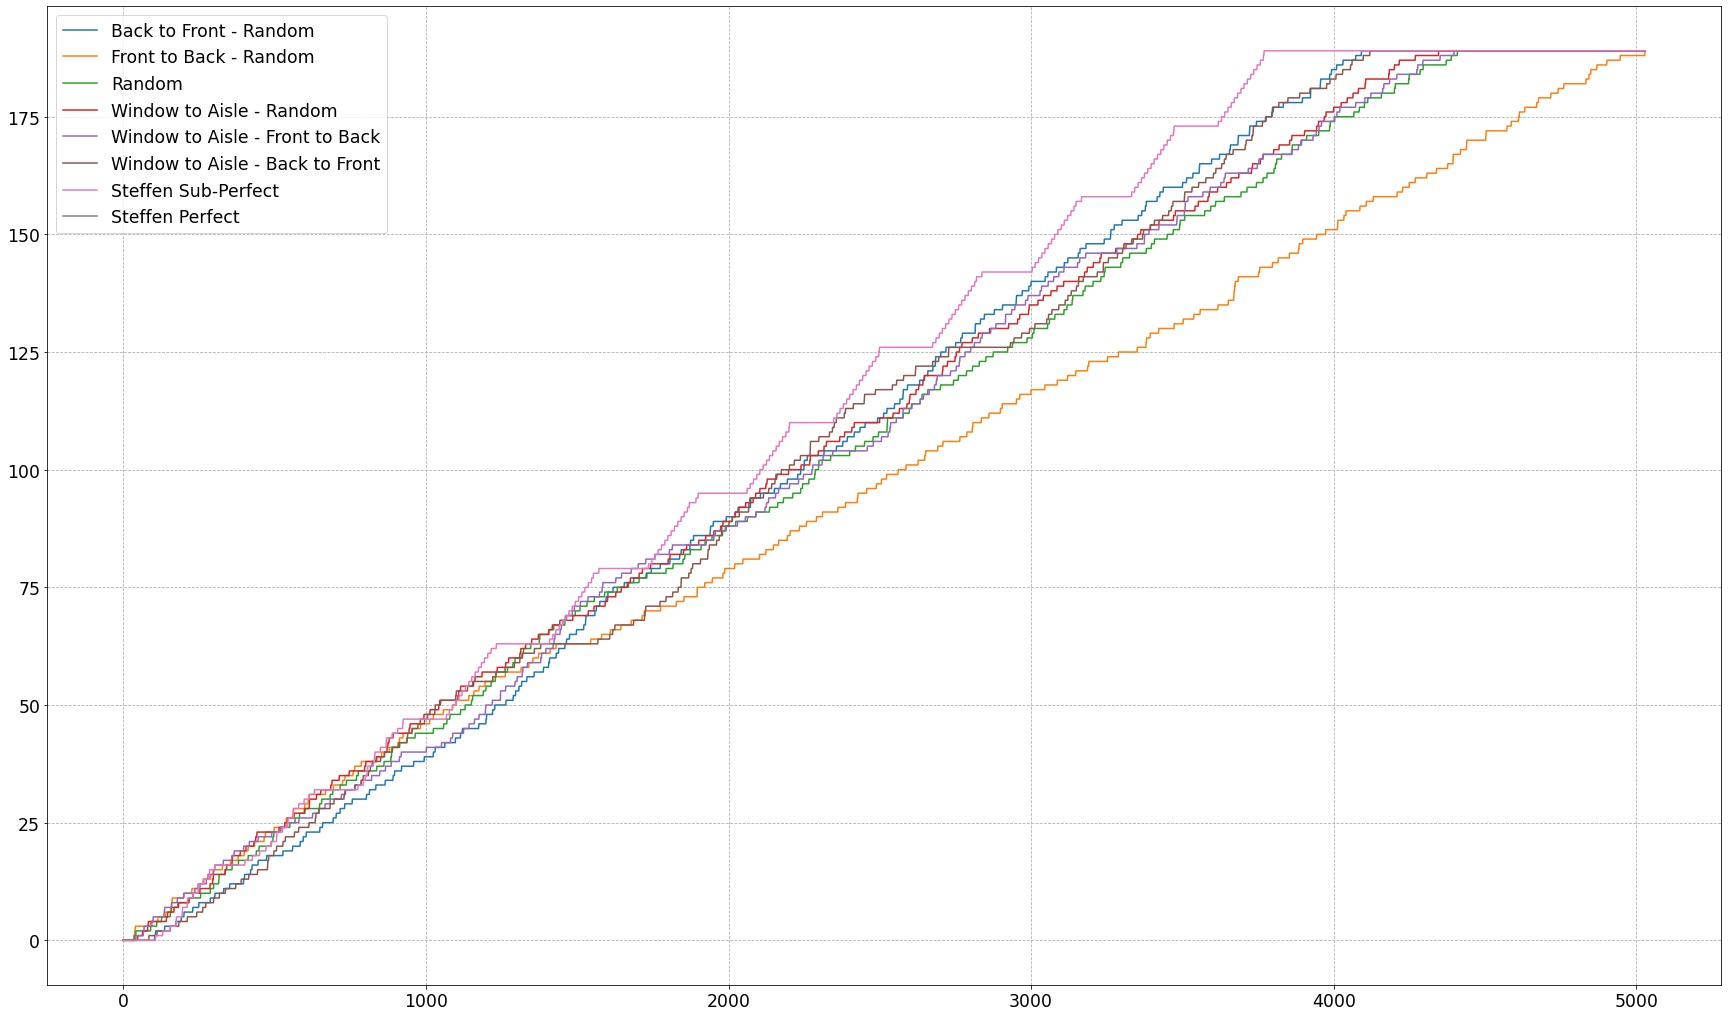
\includegraphics[width = 14cm]{speed graphs on various types.jpg}

		\small\textit{Fig. Time step comparison on different types of boarding strategies}
	\end{center}
	It's clear that the steffen sub-perfect model, which was devised by our optimization method, turns out to be the fastest strategy due to its high degree of parallelity. However, in this method, passengers in the same row are separated, therefore leading to a rather high \(\alpha_{\mathrm{satisfy}}\approx 1383.59\). What's more, the Steffen perfect method has a \(\alpha_{\mathrm{satisfy}}\) as high as \(1415.09\). Therefore we can see that both schemes sacrifice passengers' satisfaction for excessive efficiency.

	On the other hand, as previously mentioned, back-to-front and window-to-aisle are two great plans of boarding. Therefore, we decided to combine them and divide the back-to-front sections smaller. To be exact, the sections are rows, and now the passengers enter with sorted sequence. This is also our \textbf{compromised} result for the most satisfying boarding plan.

	\section{Sensitivity Analysis}
	As mentioned in \defword{Background}, there are always passengers who don't follow the instructions. Therefore, we need to make sure how much "destruction" they will cause to the boarding process.

	To define the effect, we introduce a variable $\alpha_\text{discompliance}$. It will define a certain passenger's behavior and it's generated randomly by programs. This can make our result more accurate.

	Since we've found that the dissatisfaction index of the lengthways method is too high. We  suppose that its is not appropriated for air companies. Therefore, we will mainly focus on the other three methods.

	First, we want to discover the sensitivity difference of the "random" and the "front to back" method. Their differences are shown in the table below.

	\begin{center}
	\begin{tabular}{||l|l|l||}
		\hline
		Boarding type&Time step required before&Time step required now\\
		\hline
		From front to back&5029&6558\\
		Random Boarding&4409&6241\\
		\hline
	\end{tabular}
	\end{center}

	Secondly, we mainly dicuss "back to front", which is the  best strategy  we has found now and examine its sensitivity. This time, we set random numbers of people who cause the order change and get the following result:
	\begin{center}
	\begin{tabular}{||l|l|l|l||}
		\hline
		number of uninstructed passengers&\(\Gamma\)&number of uninstructed passengers&\(\Gamma\)\\
		\hline
		24&4245&21&4516\\
		19&4096&16&4113\\
		8&4136&27&4057\\
		19&4038&11&4026\\
		13&4213&18&4144\\
		\hline
	\end{tabular}
	\end{center}

	From this we can find the following facts:
	\begin{enumerate}
		\itembf{Boarding randomly is far more sensitive than boarding from front to back.}

		This may be because the former has no order. Under this circumstance, any uninstructed behavior will disrupt the whole process more that the effect on the latter one.
		\itembf{"Back to front" method is not so sensitive to uninstructed passengers.}

		It's easy to see from the datat we've got that this method won't be effected dramatically by sudden changes and  it's time cost is still much lower  than the other one's.
	\end{enumerate}
	%\begin{center}
		%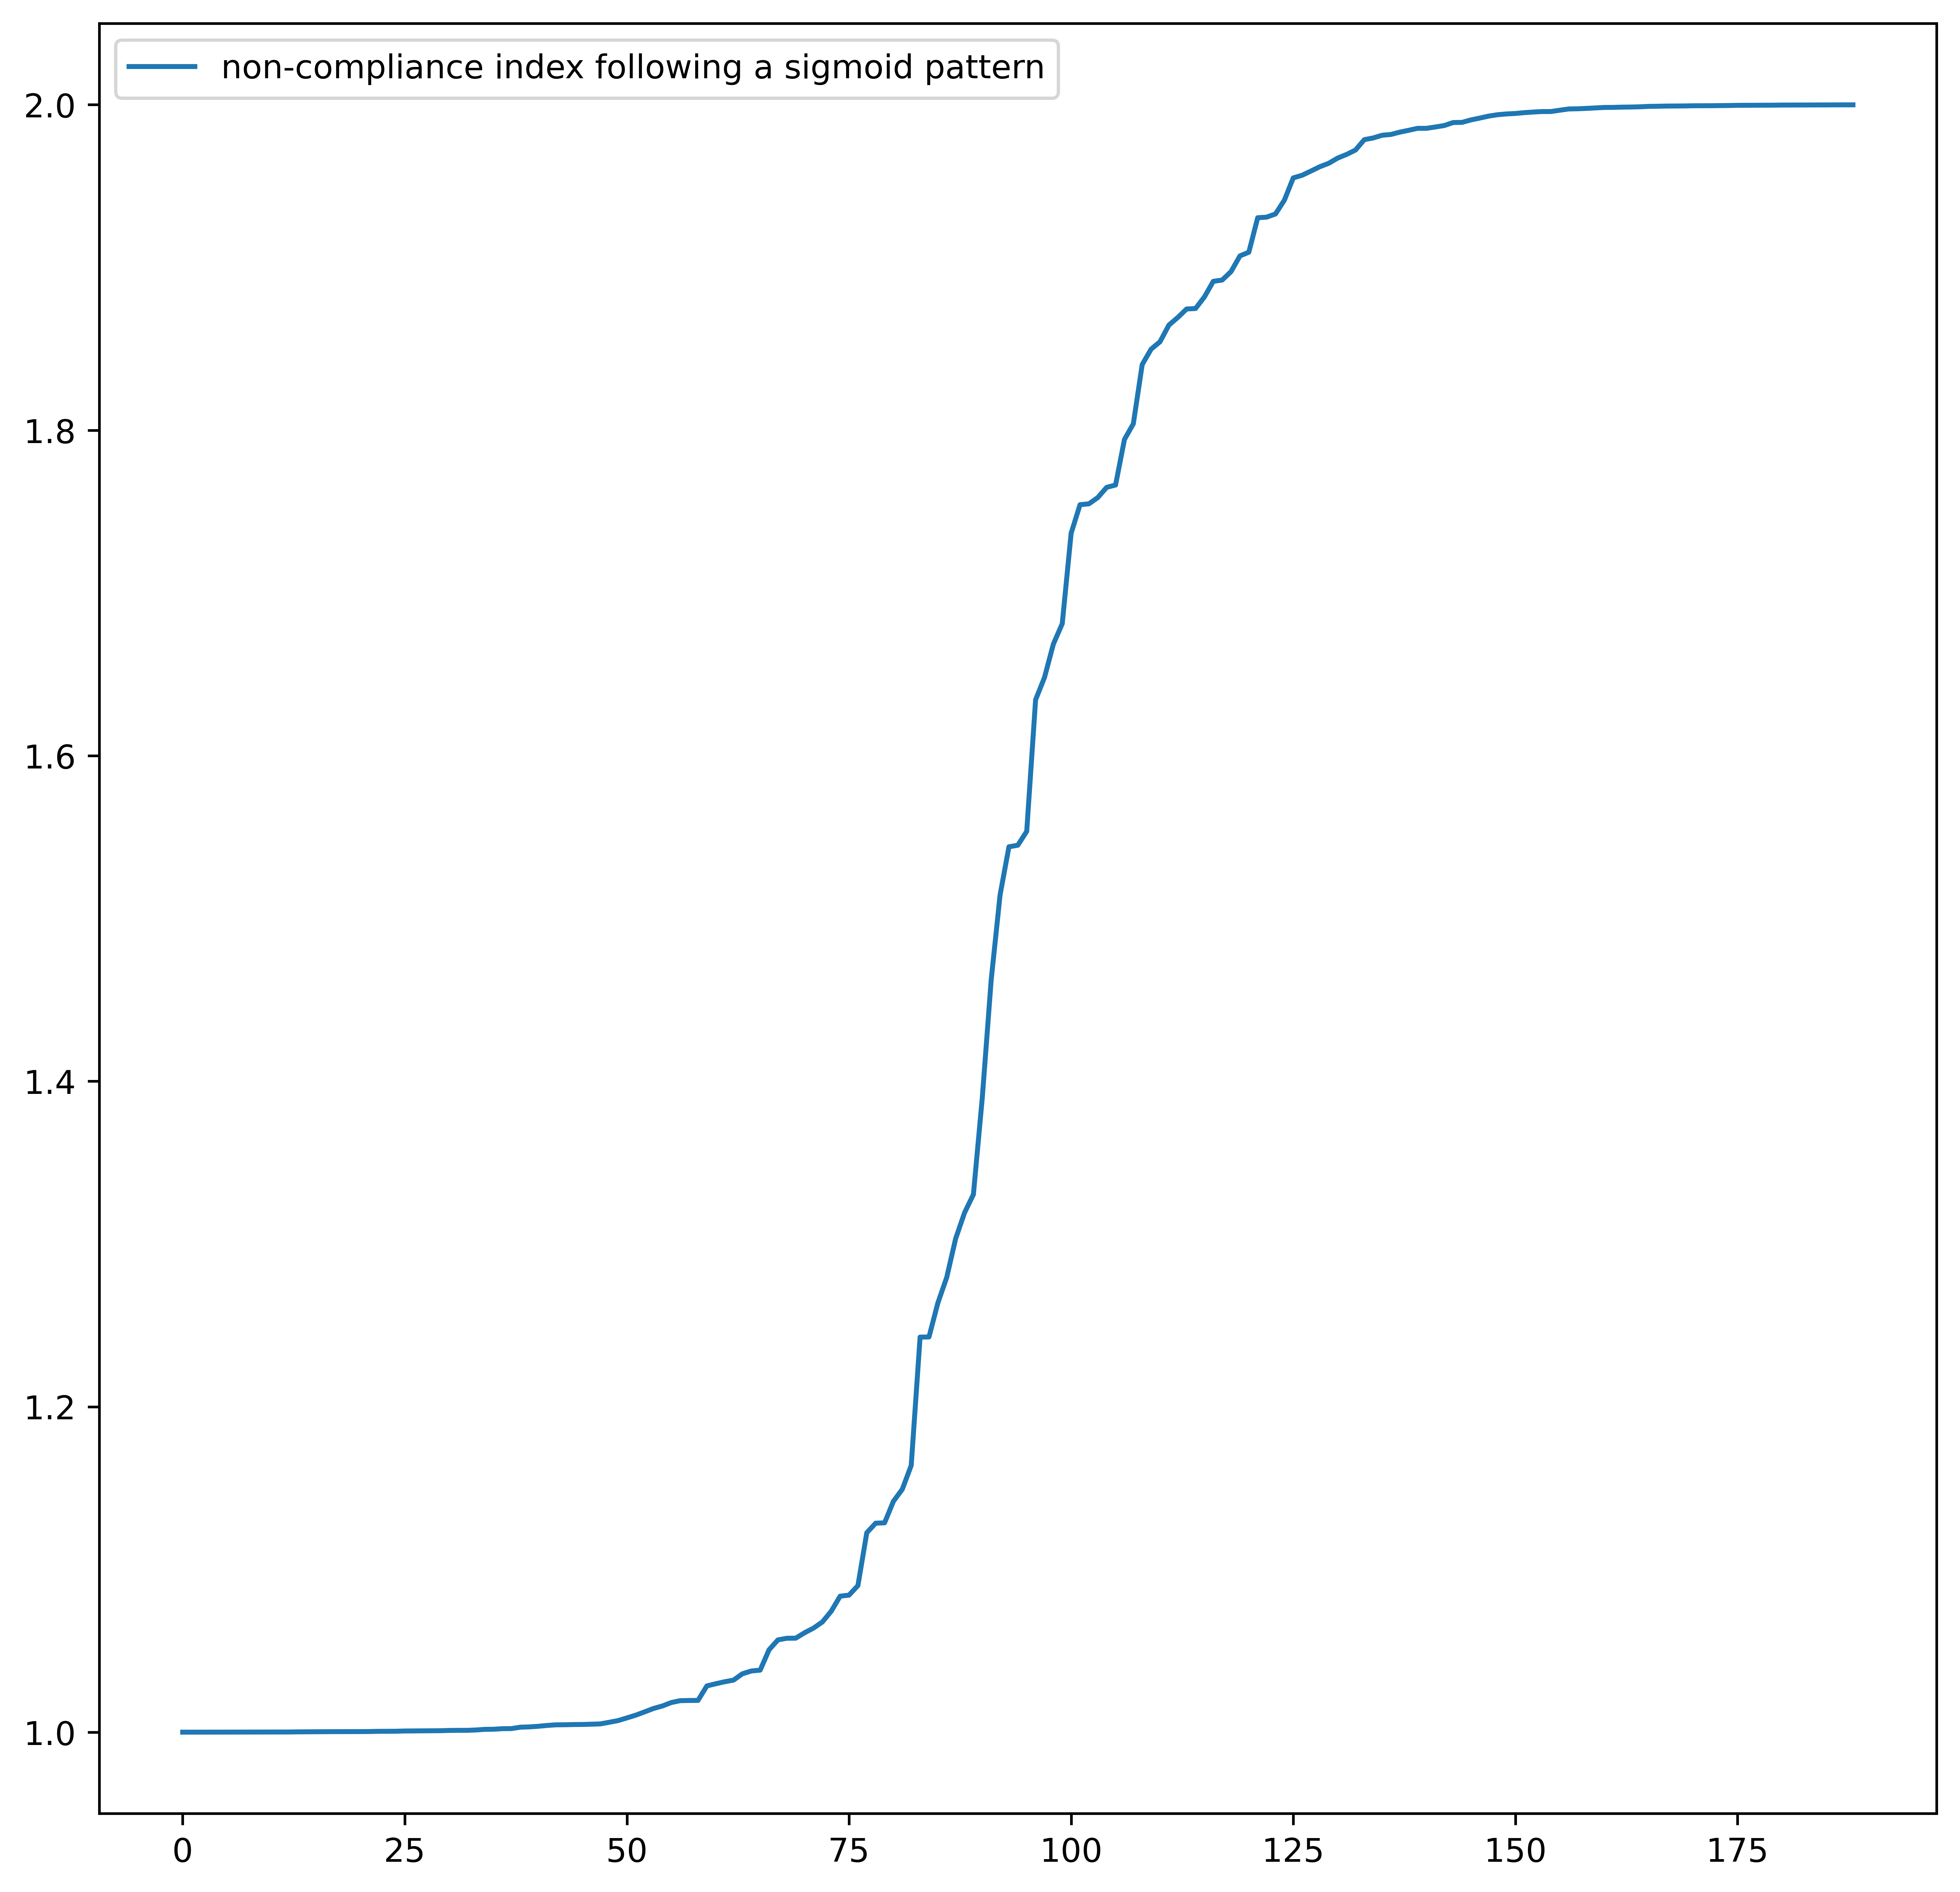
\includegraphics[width=6cm]{sigmoid.png}

		%\small \textit{Fig. }
	%\end{center}
	\section{Examining the Results}
	\begin{algorithm}
		\caption{seat}
		\begin{algorithmic}
			\STATE \# based on "back to front"
			\STATE \# initialize the index of the aisle blocks
			\FOR {an aisle block (x,y)}
			\STATE should\_occupied[x,y] = the line that block (x,y) is in \# initialize the blocks' lines
			\STATE occupied[x,y,0] = 0 \# not occupied, the third index 0 refers to the time
			\STATE \# first step: let in passengers to fill all the aisles
			\ENDFOR
			\WHILE {not all aisles are occupied by designated passengers \# there are reserved passengers}
			\STATE fill in the aisle blocks in the sequence of line 4 to line 1
			\ENDWHILE
			\WHILE {not all passengers are seated}
			\IF {someone has become seated}
			\STATE fill in equivalent passengers with the same line as the seated passengers
			\ENDIF
			\STATE update passenger status according to the assumptions and strategies
			\STATE update time
			\STATE update the occupation status of the aisle blocks
			\STATE \# Because of the existence of reserved passengers, the mobility of the central aisle could be increased, and as a result increasing the parallelism.
			\ENDWHILE
		\end{algorithmic}
	\end{algorithm}

	\subsection{Model Overview}
	In this model, we will apply our model to the images given by \# (The pictures will be shown in the next section) and find out the best strategy to them seperately. Later, we will give a brief advice about the the boarding plan. In addtion, we will list out two boarding plans that may also facilitate the air agency complete their mission and find out the efficiency of them based on our model.
	\subsection{Notation}
	\begin{center}
	\begin{tabular}{|l|l|}
		\hline
		$\sigma_i$&the best strategy for section $i$\\
		\hline
		$A_{i,j}$&passenger $A$ whose seat is in $\left(i,j\right)$\\
		\hline
		$\eta_i(t)$&efficiency of $L_i$ at $t$\\
		\hline
		$\alpha_\text{loaded}$&loaded index\\
		\hline
	\end{tabular}
	\end{center}
	\subsection{Short Passenger Cabin}
	The problem of not having enough space for aisles is actually easy to solve. Same as the disembarking process, if all the passengers are put into order and  are stuffed in the aisle. Thier speed won't be affected. Moreover, we can find that  the whole lengths of this plane has been reduced, which means $T(A)$ won't change dramatically. The only difference may be the seats have been narrower, which  means $\varepsilon(A)$ has decreased. Therfore, we  can without doubt use  the same strategy as the normal plane types.
	\subsection{Flying Wings}
	Flying  wings is a special kind of plane. Different from others, it's especially spacious and can accomodate a great number of people. It's shape is shown below.

	Though we define the plane as several rectangle cells, passengers can still travel in arctangles in this kind of plane. We can find that:
	$$\left| s_{\mathrm{prev}}-s_{\mathrm{now}} \right|=\left| d\sqrt{x^2+\left( \frac{7}{2}d \right) ^2}-\left( x+\frac{7}{2}d \right) d \right|\\\le \left| d\sqrt{l^2+\left( \frac{7}{2}d \right) ^2}-\left( l+\frac{7}{2}d \right) d \right|\\=\frac{18-2\sqrt{53}}{5}\approx 0.688\mathrm{m}\\$$

	This number is even smaller that 1 second. Therefore, we willnot consider this change.


	\begin{center}
		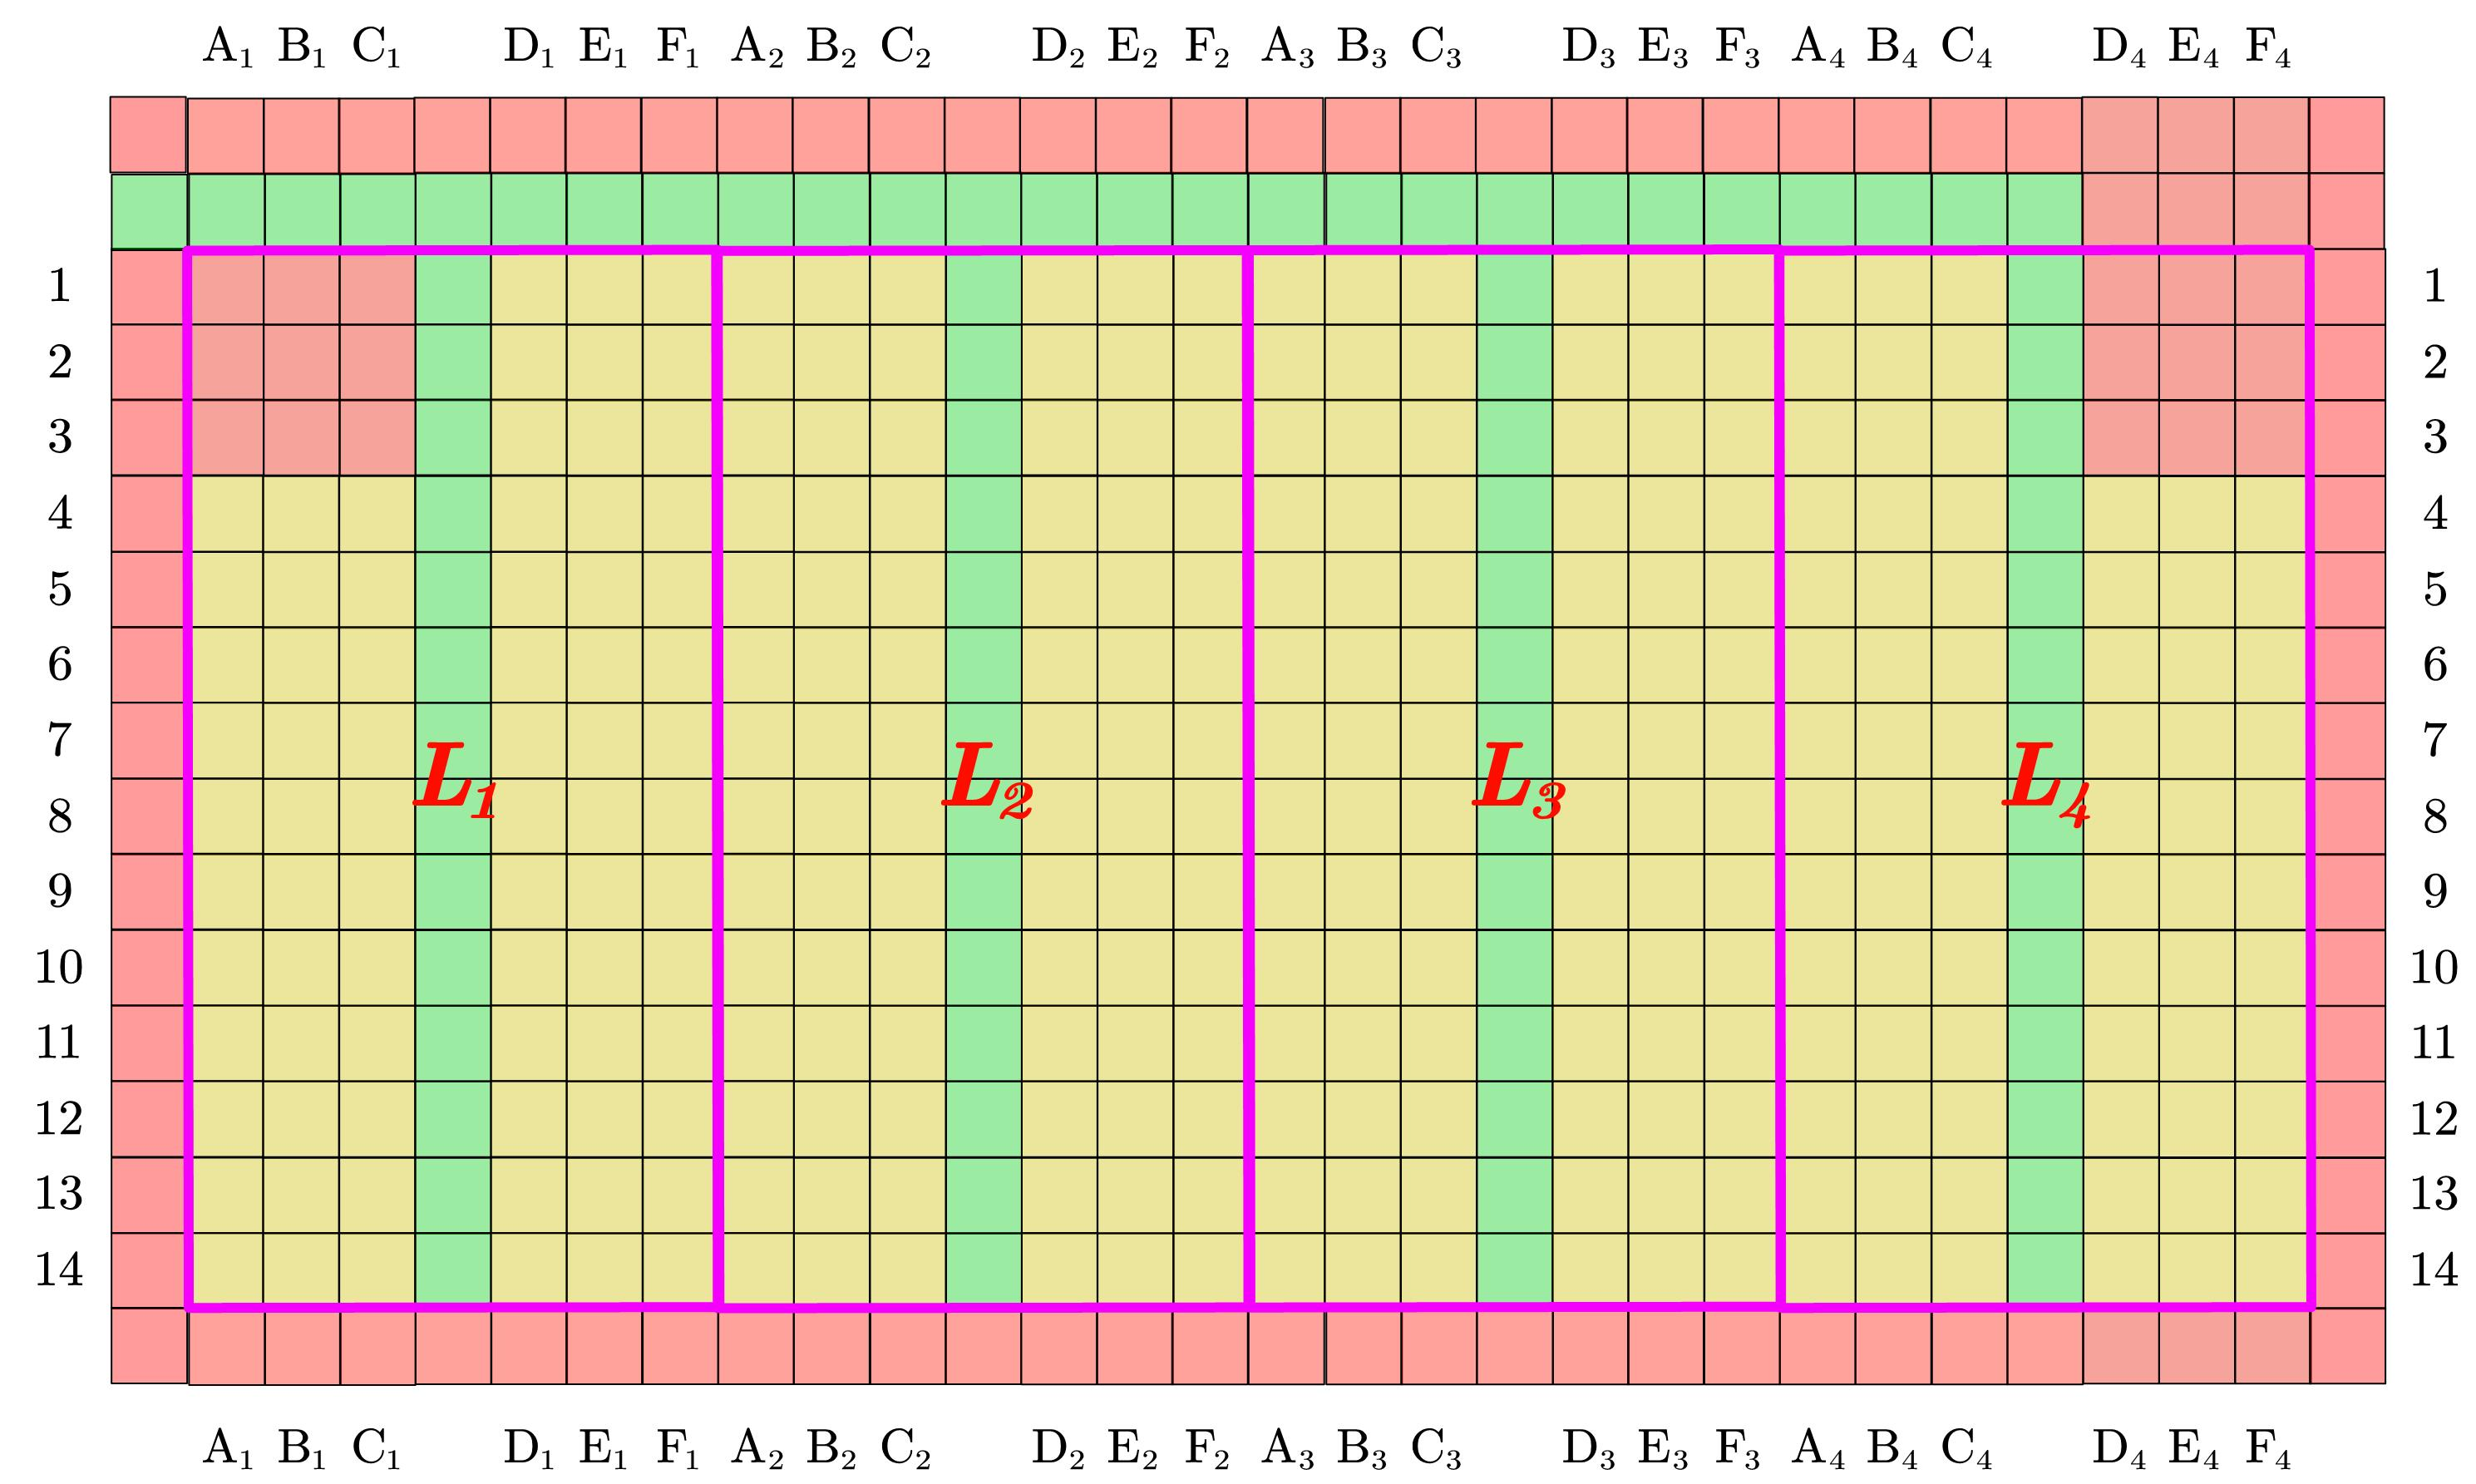
\includegraphics[width=12cm]{flyingwings.jpg}

		\small \textit{Fig. Flying Wings}
	\end{center}

	As can be seen in the graphics, we divide the plane into four parts and we will calculate the time used seperately.In one certain section, we define the set of passengers $P_i=\left\{A_{1,1},A_{2,2},A_{3,3}......A_{i,M_i}\right\}$. It's clear that every part is independent and order-preserving, which means that the best plane can only be affected by the passengers' condition for any initial interval. Therefore, we can get a brief formula about the best strategy:
	\[\sigma_i (\rho_i): \left\{1,..., any \mathbb{Z}^+\right\}\rightarrow^{\sigma_i} \left\{1,..., any \mathbb{Z}^+ \right\}\]

	It means that passenger $A_{i,j}$ will have the order number in $\sigma_i (j)$. ($i=1,...S, j=1, \left|P_i \right|=M_i$)

	In addtion, we introduce $\eta_i (t)$ to assess the efficiency of $L_i$ at $t$. The less cells in the general aisle is required, the bigger $\eta_i (t)$ is. And the more cells in the branch aisles and the bigger parallelism ($r_i (t)$) is, the bigger $\eta_i (t)$ is.

	According to this standard, we propsoed two claims:
	\begin{enumerate}
		\itembf{Every passenger should keep himself close to the paassenger in front of him.}

		As the aisle is so narrow that it can only allow one passenger to pass at the same time, we don't need to take the passengers' passing each other into consideration. Under this assumption, we need to find a best strategy for passengers to go through the aisle and get to their own seats. The fastest strategy for the first passenger to board is obviously passing the aisle at the fastest speed to get to his/her seat. And for the other passengers, as they can never pass the passenger ahead, the farthest distance they can reach in $m_0$ time steps is less than that of the passenger ahead (because he/she could only stick tight to the passenger ahead and behind that passenger). As a result, we can get that the quickest strategy for every passenger to get to his/her seat is to stick tight to the previous passenger until reaching his/her own seat.
		\itembf{The most ideal way is to stuff the aisles full of passengers.}

		We can see from the map that there are several aisles in the plane. If we want to maximize the time cost, we must make full use of the space. Based on this claim, our work is actually to find the circumstances where the aisles are stuffed with passengers.Therefore, we introduced the loaded index $\alpha_\text{loaded}$ to describe it's condition (which will be explained in detail in the following part). It will facilitate our calculation: given that the order in this plan is certain, there are only $S$ kinds of ways to determine the boarding time of the next passenger, which will be easy to enumerate.
	\end{enumerate}
	\subsubsection{ Calculating \(\alpha_\text{loaded}\)}
	As mentioned above, $\alpha_\text{loaded}$ is an important factor in our plan. The index serves for two purposes.
	$$
	\begin{cases}
		\text{general: prevent the aisle from being stuck}\\
		\text{branches: have small impact on branches}
	\end{cases}
	$$
	\subsection{Two Entrance, Two Aisle}
	In the Two-Entrance-Two-Aisle Plane, we found that the seats aren't "simply organized" (the DEF seats at row 24 even seem to be at row 25). Therefore, we reorganized the seats into our cells, as mentioned and modeled above. Due to the assumption that passengers in better classes enter first, we first open the front entrance to let business passengers in (rows 1-3). To be exact, each aisle will have half of the passengers flow and we can divide the business class into two "2+1" single-aisle aircraft and apply on our models mentioned above. As there are not many passengers in the Business Class, different ways of boarding will not cause big difference in the total boarding time.

	Next, we consider the economy class. We recognized that rows 25 and 26 are missing D, E and F, so we simply turned them into walls to ensure the simplicity of the aircraft model. However, while dividing the aircraft into the "front half" and the "latter half", we will still consider these walls as "seats with no passengers", as the walking distance in the aisle may cause big difference to the whole time used. We will use row 30 as the division row (the mean of 12 and 47) while applying it to the front half to equal the passengers the best.

	Dividing each half into two parts, "upper part" and "lower part" is not an easy thing to do, as in the middle, the seats are not symmetric - D, E, F make an odd number. To maximize the equality of the two parts, we decided to assign passengers in odd rows to the upper part while passengers in even rows to the lower part.

	Similar to the "Flying Wing", we would take the boarding strategy that could make the best use of aisle space. Since the two parts don't bother each other, it's clear that $\Gamma=\max \left\{\Gamma_\text{former}, \Gamma_\text{latter}\right\}$. The picture below shows the map we've drawn of the latter part of this plane.

	\begin{center}
		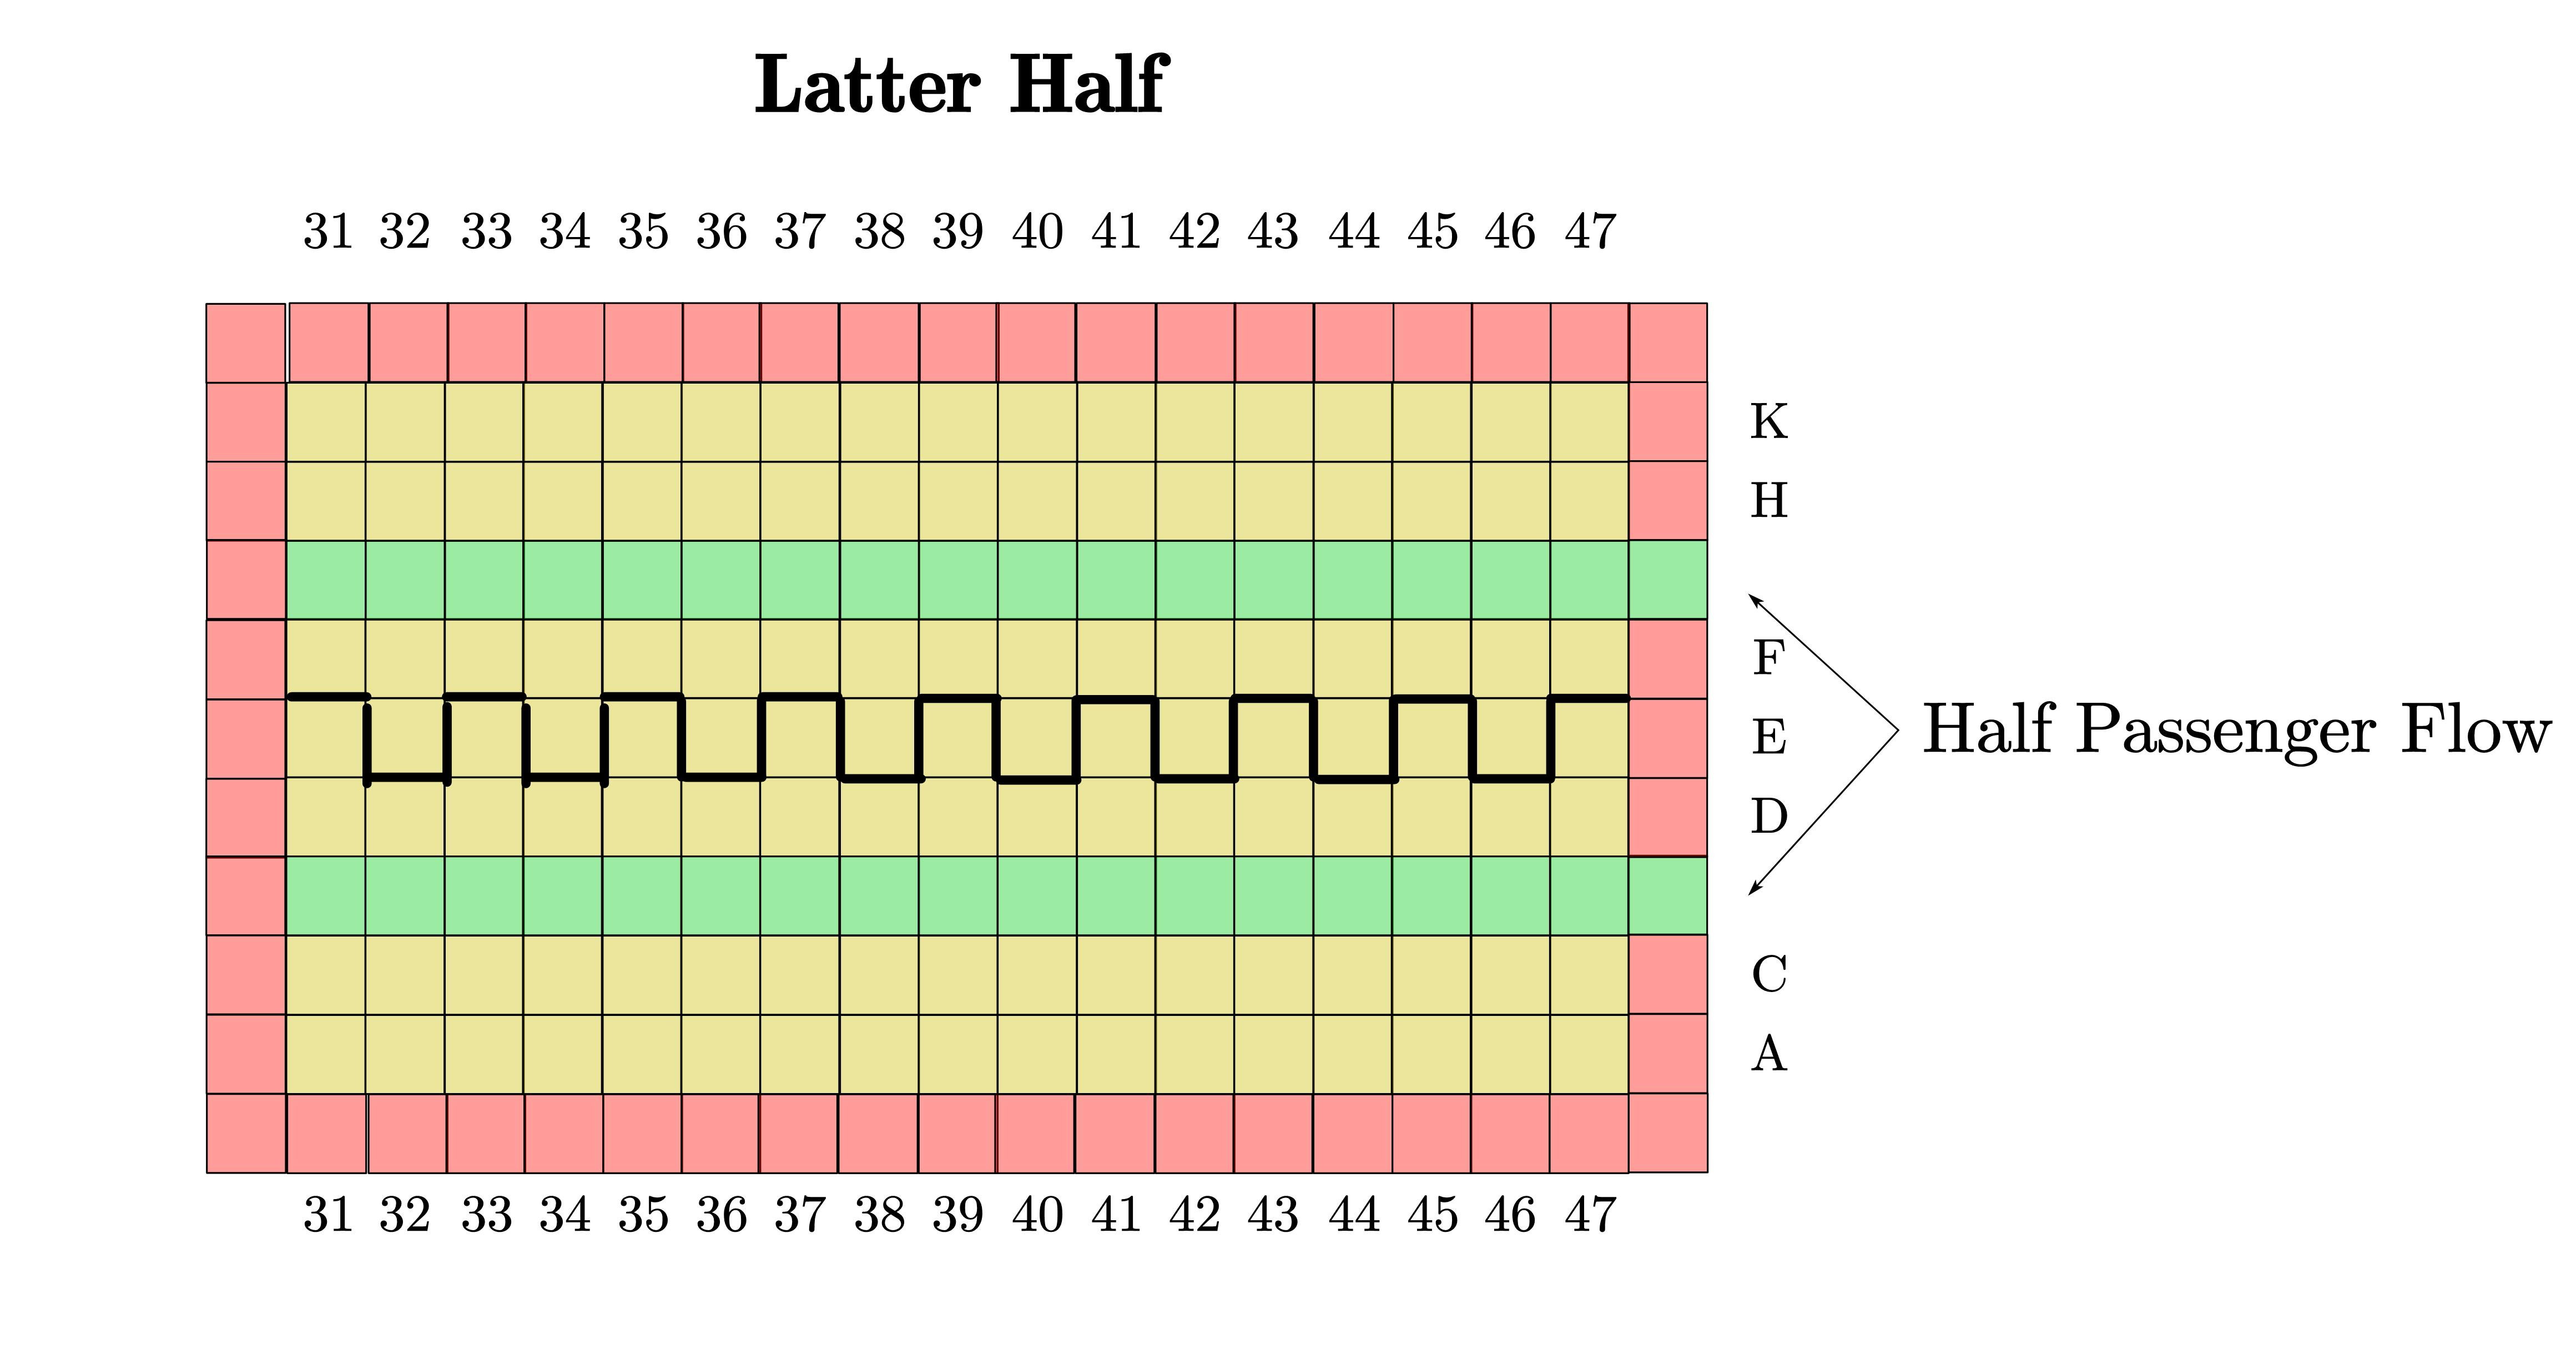
\includegraphics[width=11cm]{double.jpg}

		\small \textit{Fig. map of two entrance, two aisle plane}
	\end{center}

	After calculation by progams, we find that the boarding time of the first half is 2026 time steps while that of the latter half is 1862 time steps. So the final result is 2026 time steps.
	\section{Strengths and Weaknesses}
	\subsection*{Strengths}
	\begin{itemize}
		\itembf{Accuracy}

		In our model, we take several special situations into consideration. Also, we use several programs to facilitate our calculation. This makes our result reasonable and precise.
		\itembf{Universality}

		In our model, we succeeded in achieving visualization of the plane and  successfully simulated the whole process of different boarding methods (Some of the examples are shown in \defword{Appendix}).  This means that our model can be applied to a variety of problems.
	\end{itemize}
	\subsection*{Weaknesses}
	\begin{itemize}
		\itembf{Complexity}

		We introduce a great many variables and a variety of explanations in our model. This will make our model more complex and less easy to understand.
		\itembf{886 }
	\end{itemize}




	\newpage
	\section{Letter to the Airline Executive}
	\noindent Dear airline executive:

	We are the \defword{IMMC Mathematical Modeling Group}. We've heard that you have problem on saving time and raising efficiency of boarding and disembarking. In our opinion, this may be caused by the inefficiency of the boarding and disembarking plan you have used. It gives us great pleasure to give some suggestions to you  about these two process based on our model.

	To begin with, we want to talk about boarding. whatever kind of strategy your company adopts, it's crucial that the features below are taken into account:

	\begin{itemize}
		\itembf{Stability.}

		While minimizing total boarding time, the model itself must be solid enough, or in other words, the strategy itself should not change while the relative parameters of passengers change. (For example, even when some passengers bring more luggage with them, it's important to keep the model as it originally was.) The more structured your boarding strategy is, the less an impact will variations in these passenger-based parameters have on the overall time of boarding.
		\itembf{Hommization.}

		Firstly, try a boarding way that minimizes the time a passenger offers his/her seat, and thus lowering anxiety and annoyance of unnecessary seat-offering. Therefore, it's crucial to make sure that the overall boarding process generally lets passengers near the window board first, and lets those next to the aisle board last. As a result, passengers can get seated with satisfaction and pleasantly start the journey.

  		Secondly, make sure that families or friends board in succession. To be more specific, please first check whether passengers in the same line are put together, as passengers familiar with one another tend to choose adjacent seats. What's more, families with the young should righteously board together.
		\itembf{Efficiency.}

		Nobody likes being stuck in a queue for too long. Therefore, with stability and hommization taken into consideration, please choose the option with the least queuing time (also equivalent to the least overall boarding time). For instance, under the single-aisle scenario, front-to-back boarding is catastrophic, since each person stowing his/her luggage causes a 'fullstop', with latter passengers not even on the plane, and therefore can do nothing but wait.

		And with these three factors combined, we get a solution! We call it 'Back to front, section by section, and window middle aisle'.

		Before boarding, each passenger should first get a 'boarding' number. We suggest the plane be divided into three sections, with boarding sequence from back to front (boarding number 1, 2, and 3). For each group of passengers with the same boarding number, group them by row, also back to front, so that more passengers can board at the same time. The following diagram gives the optimal strategy:
		\begin{center}
			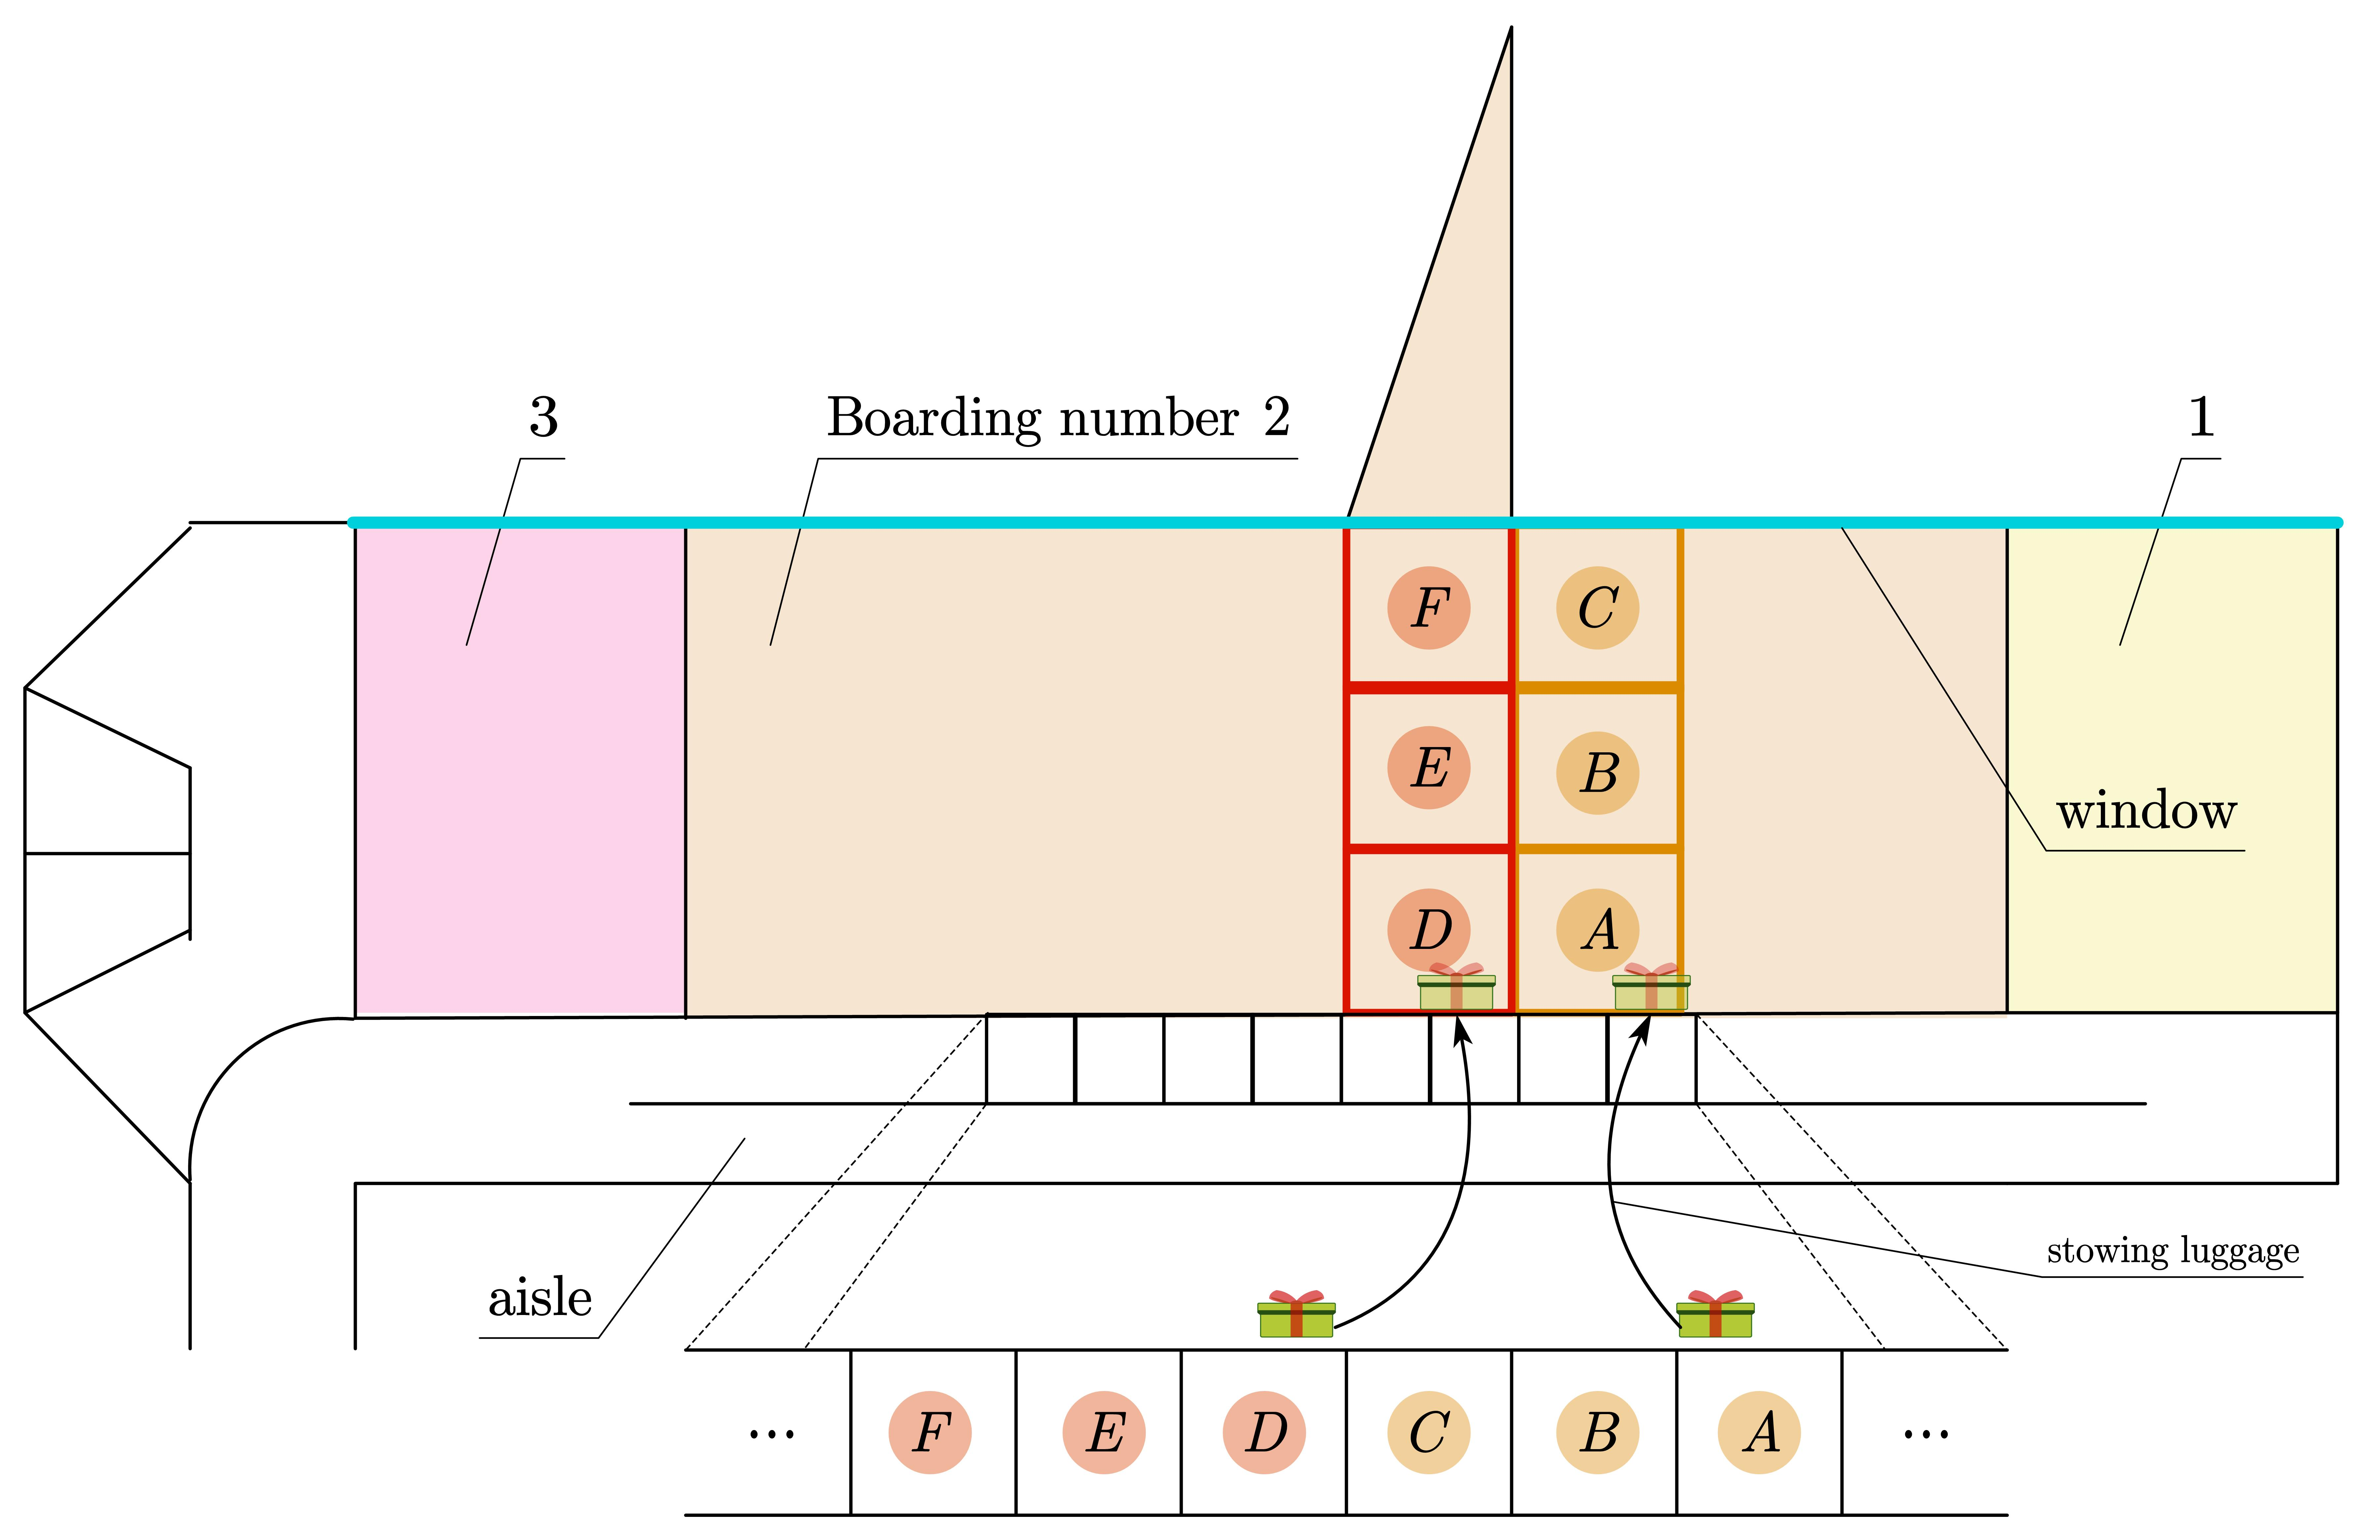
\includegraphics[width=11.6cm]{advice.jpg}
		\end{center}
	\end{itemize}

	Also, here are some small tips we've concluded from our model:
	\begin{enumerate}
		\itembf{If there are several aisles in your plane, avoid blocks in general aisles.}

		General aisles are especially important in the whole boarding process. It actually controls other branch aisles. If too much people in the general blocks the way, it may lead to a thorough collapse of this process. Therefore, you must make sure the general aisles are blocked.
		\itembf{Divide the plane into several sections.}

		If your plane map is especially complicated, don't worry about it! Divide the whole plane into several parts according too it's geometric shape and find out the best strategy seperately based on the suggestions we've given above. Later, combine them all together and implement them seperately.
		\itembf{Provide enough space  for luggages.}

		Nowadays, to save cost on consignment, many passengers may choose to bring their luggages with them to the plane. If there isn't enough place for luggages, passengers may spend more time on dealing with their luggages. This means more time for others in waiting, which will lead to an increase in the total boarding time (caused by queuing) and a rise in passengers' negative emotions.
	\end{enumerate}

	As for the disembarking part, our suggestion is that you needn't worry much about it. According to the result we've got, the best plan is actually let passengers get "stuck" in the aisle in order! Under this circumstance, all that you need to do is actually let the passengers bear their seat number in mind. Passengers first grab their bags, and get into the aisle from front to back, aisle to window, ensuring that lines are kept together and that the aisle is always full.

	Hope that our suggestions can help you, looking foward to your reply!

	\noindent Yours sincerely,

	\noindent \defword{IMMC Mathematical Modeling Group}


	\newpage
	\thispagestyle{empty}
	%\setcounter{page}{\wholepages}
	\renewcommand\refname{References}
	\addcontentsline{toc}{section}{References}
	\tolerance=500
	\begin{thebibliography}{100}
	\bibitem{passenger} \textit{Lorentzian-geometry-based analysis of airplane boarding policies,highlights “slow passengers first” as better},
	Sveinung Erland, Jevgenijs Kaupužs, Vidar Frette, Rami Pugatch and  Eitan Bachmat
	\bibitem{steffen} \textit{The best way to load a passenger plane}, Jason Palmer\\
	https://www.bbc.com/news/science-environment-14717695
	\bibitem{greenshields} \textit{Greenshields Model}, Traffic Theory\\
	https://www.webpages.uidaho.edu/niatt\_labmanual/\\chapters/trafficflowtheory/theoryandconcepts/GreenshieldsModel.htm
	\end{thebibliography}

	\newpage
	\thispagestyle{empty}
	\renewcommand\refname{Appendix}
	\tolerance=500
	\Huge \textbf{Appendix}
	\\[0.8cm]
	\normalsize These graphics are mainly about the visualized results we've got in our model.
	\\[2pt]
	\large \textbf{Back to Front}
	\begin{center}
		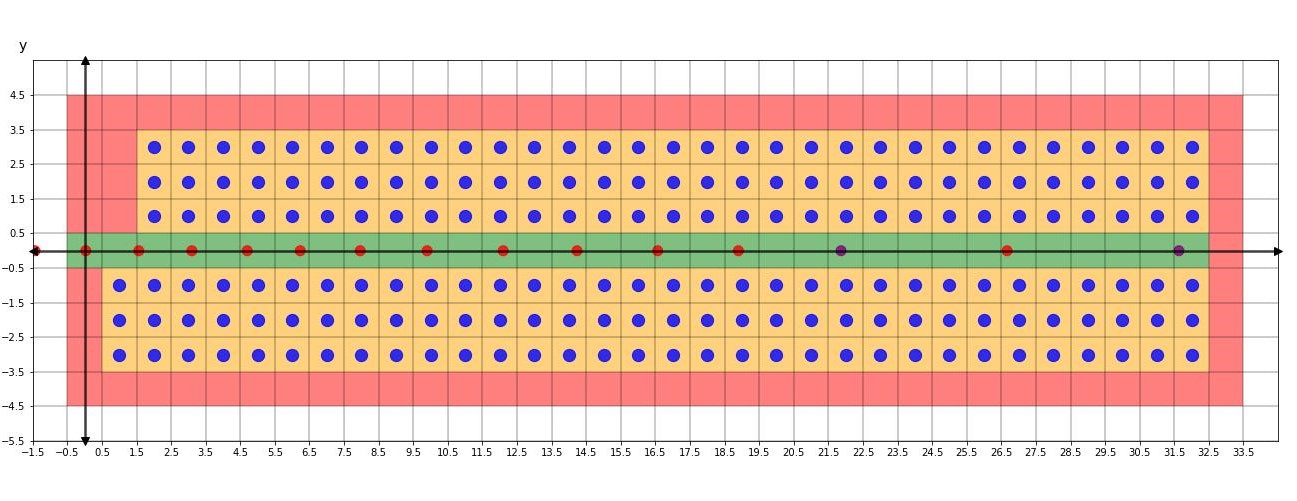
\includegraphics[width=14cm]{backtofront1.jpg}\\
		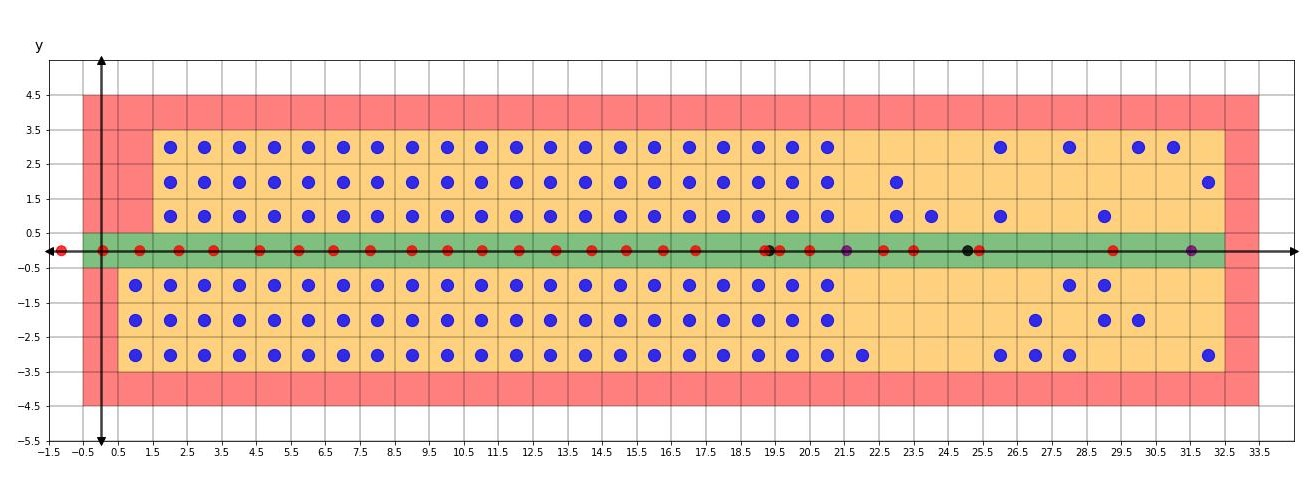
\includegraphics[width=14cm]{backtofront2.jpg}\\
		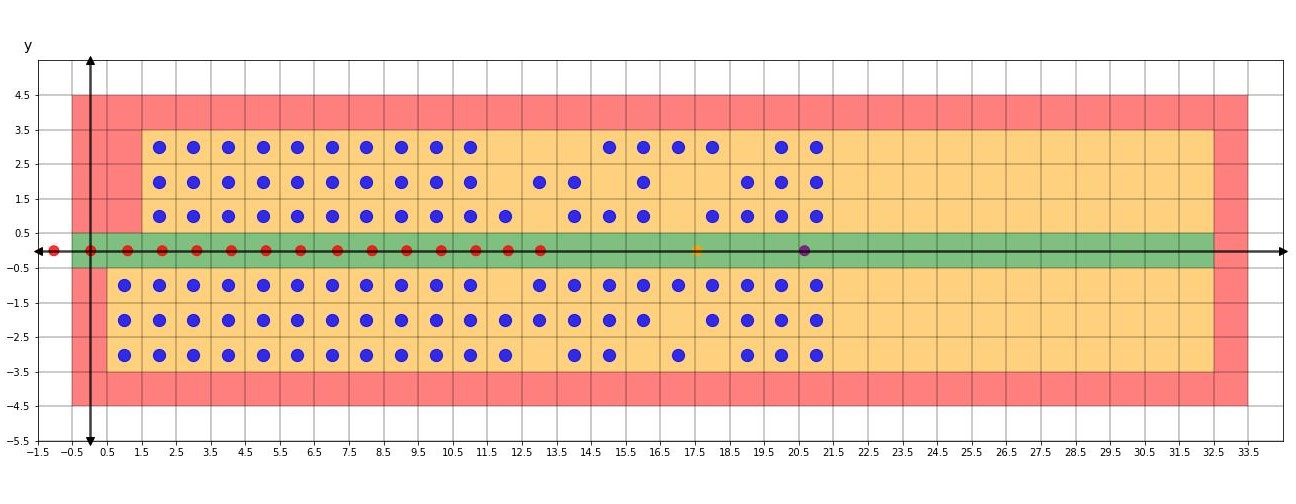
\includegraphics[width=14cm]{backtofront3.jpg}\\
		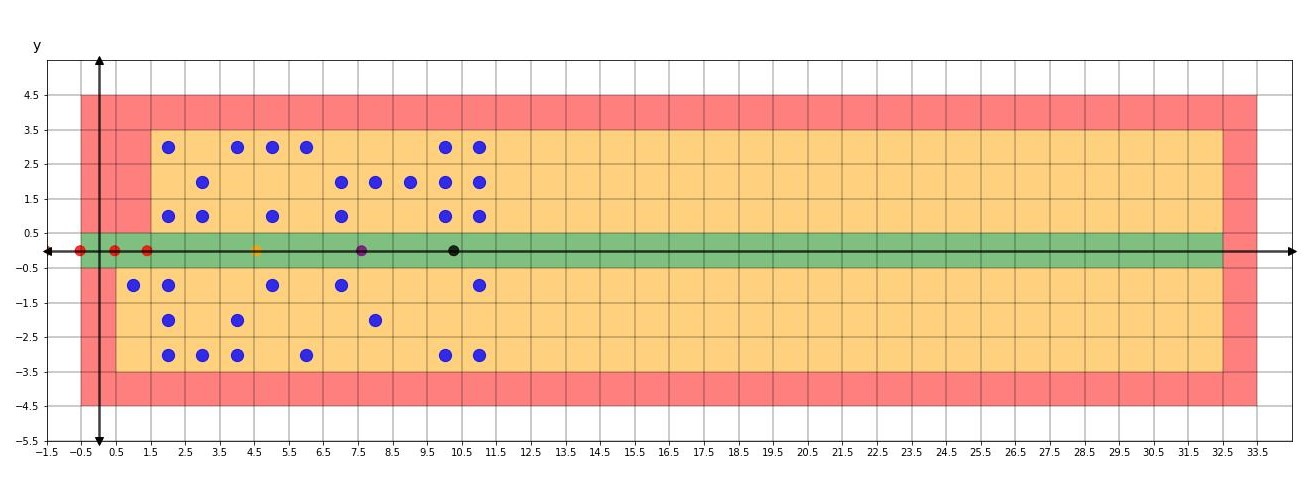
\includegraphics[width=14cm]{backtofront4.jpg}\\
	\end{center}
	\large \textbf{Window Middle Aisle}
	\begin{center}
		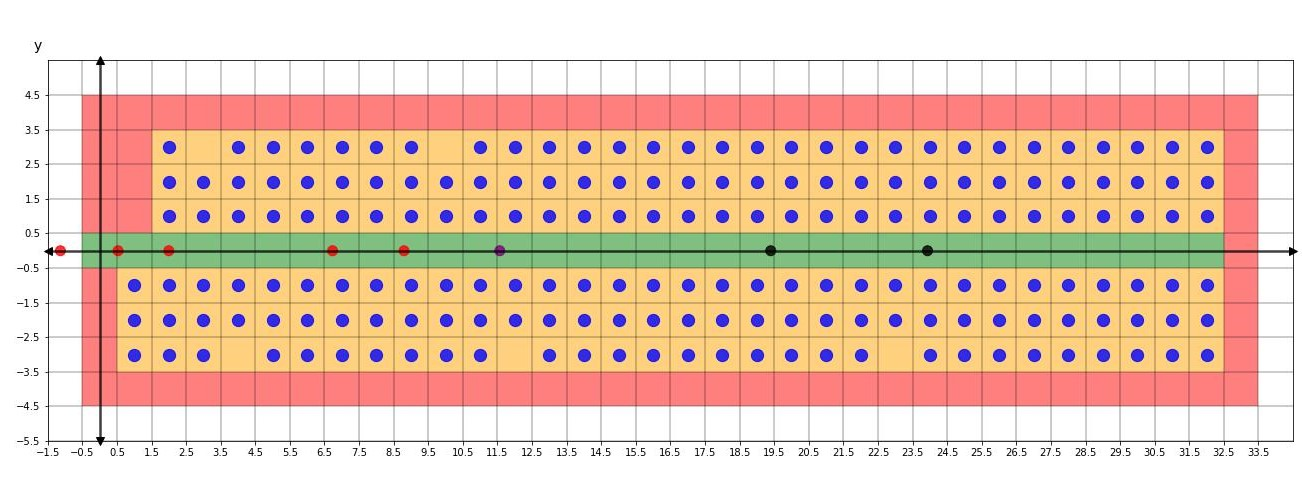
\includegraphics[width=14cm]{wdmd1.jpg}\\
		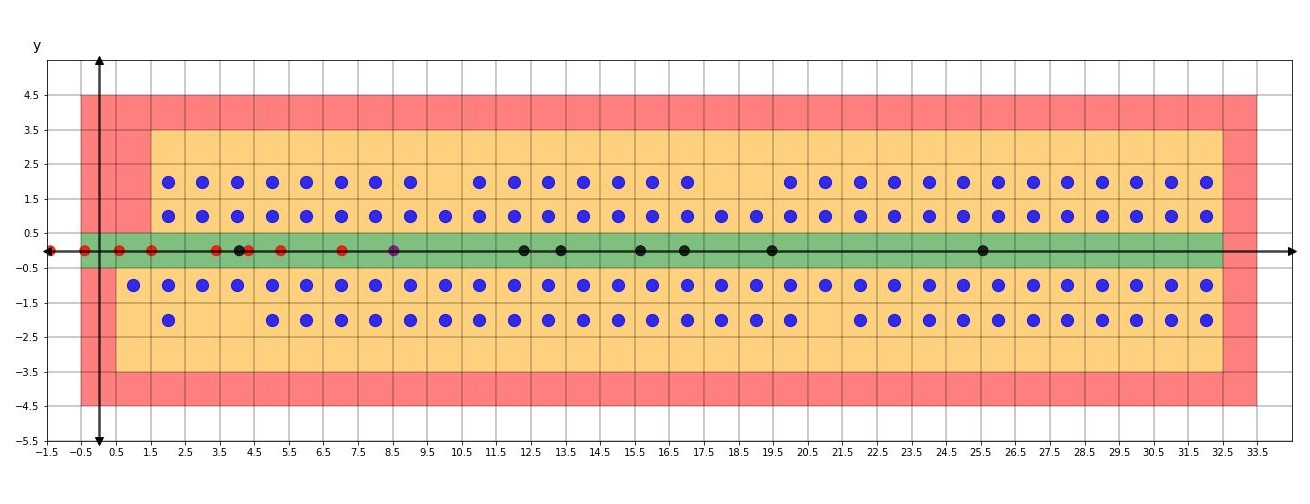
\includegraphics[width=14cm]{wdmd2.jpg}\\
		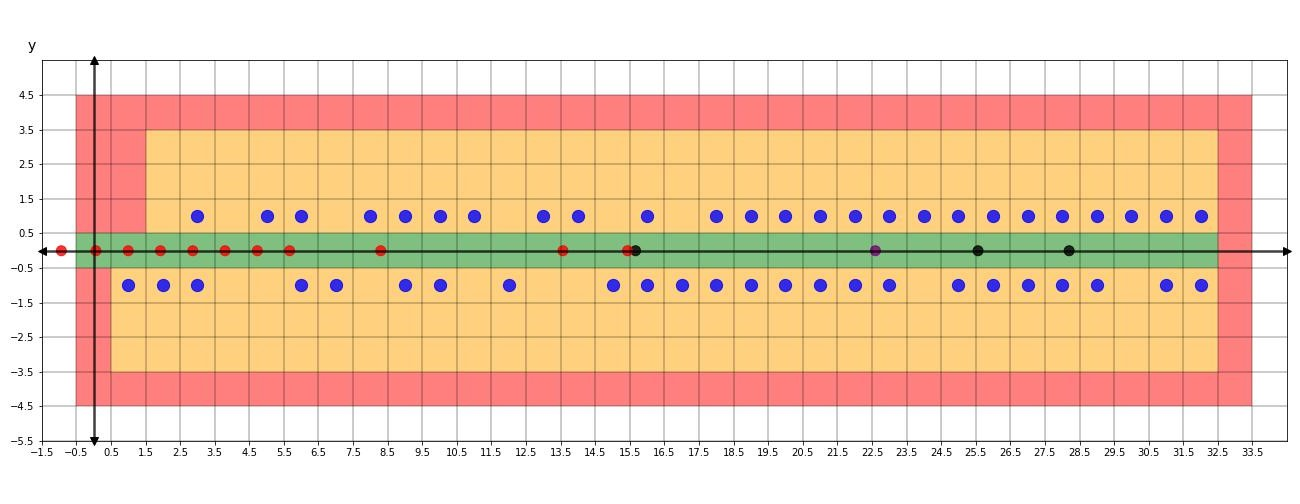
\includegraphics[width=14cm]{wdmd3.jpg}\\
	\end{center}
	\large \textbf{Random}
	\begin{center}
		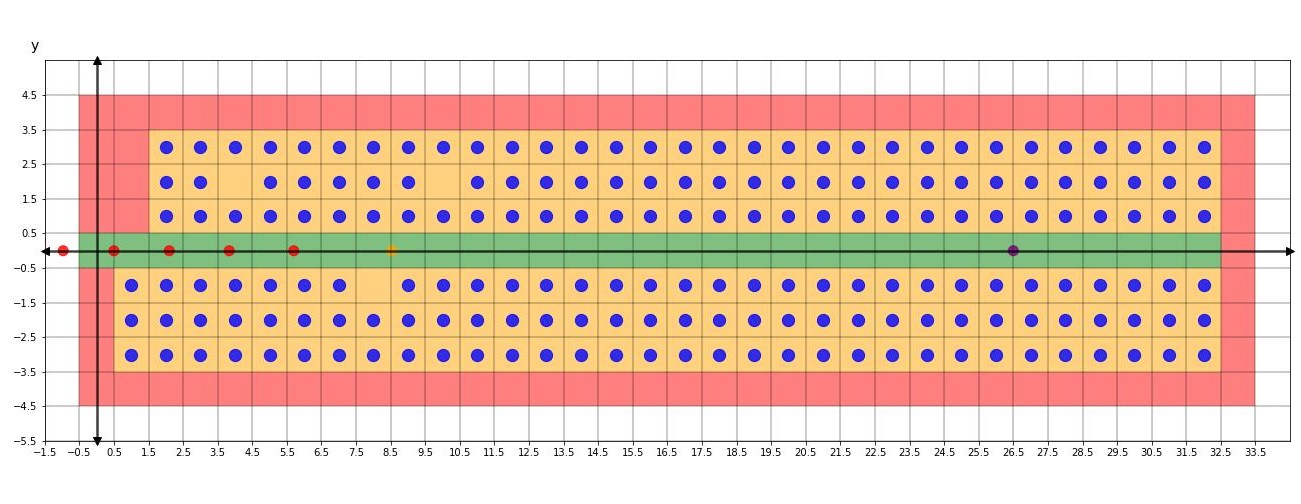
\includegraphics[width=14cm]{random1.jpg}\\
		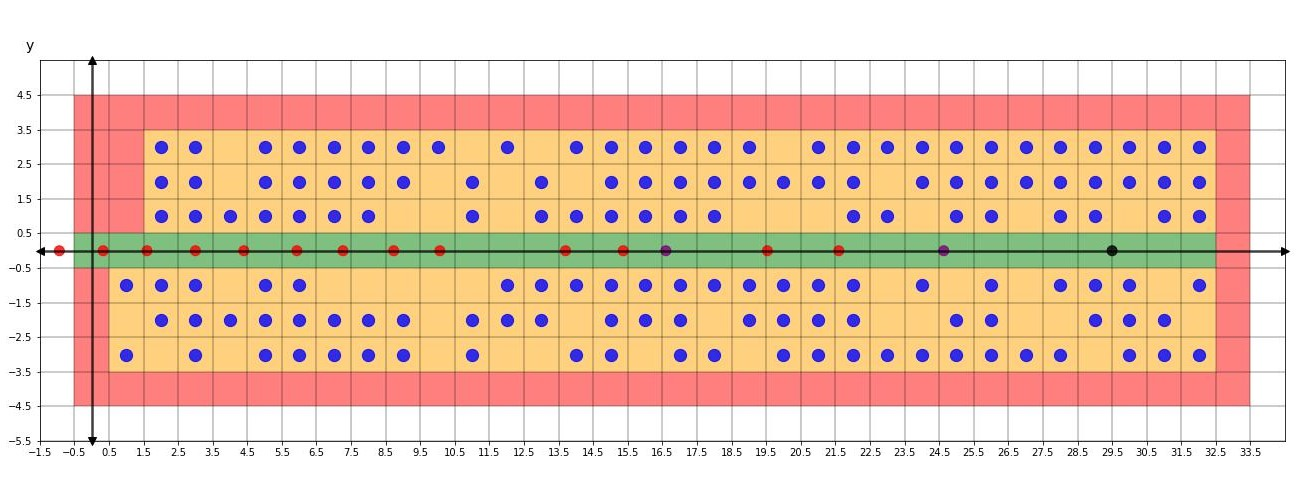
\includegraphics[width=14cm]{random2.jpg}\\
		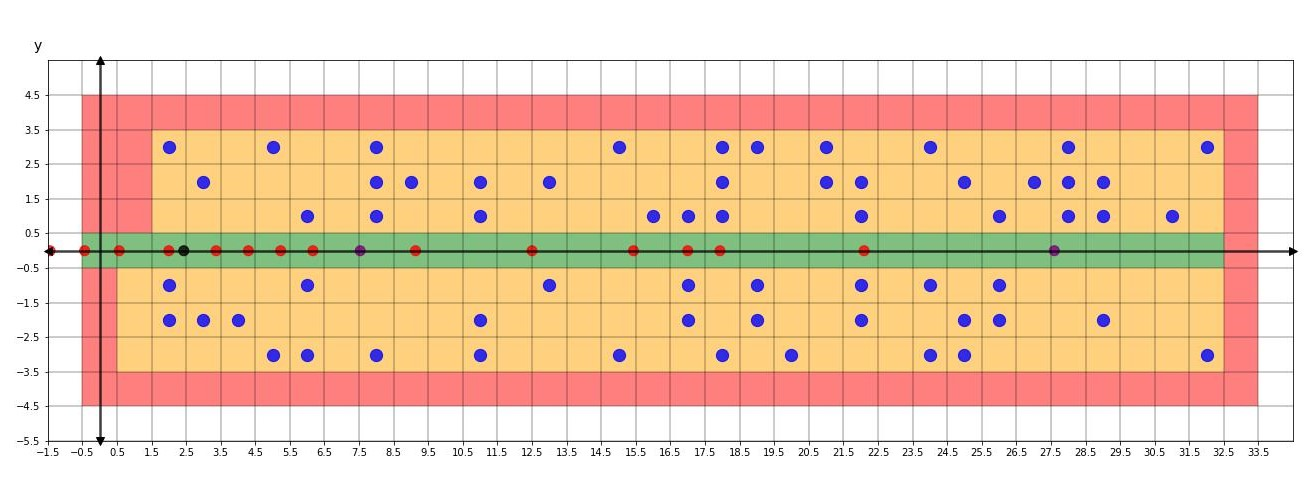
\includegraphics[width=14cm]{random3.jpg}\\
	\end{center}
	\large \textbf{Two Entrance, Two Aisle (three forms)}
	\begin{center}
		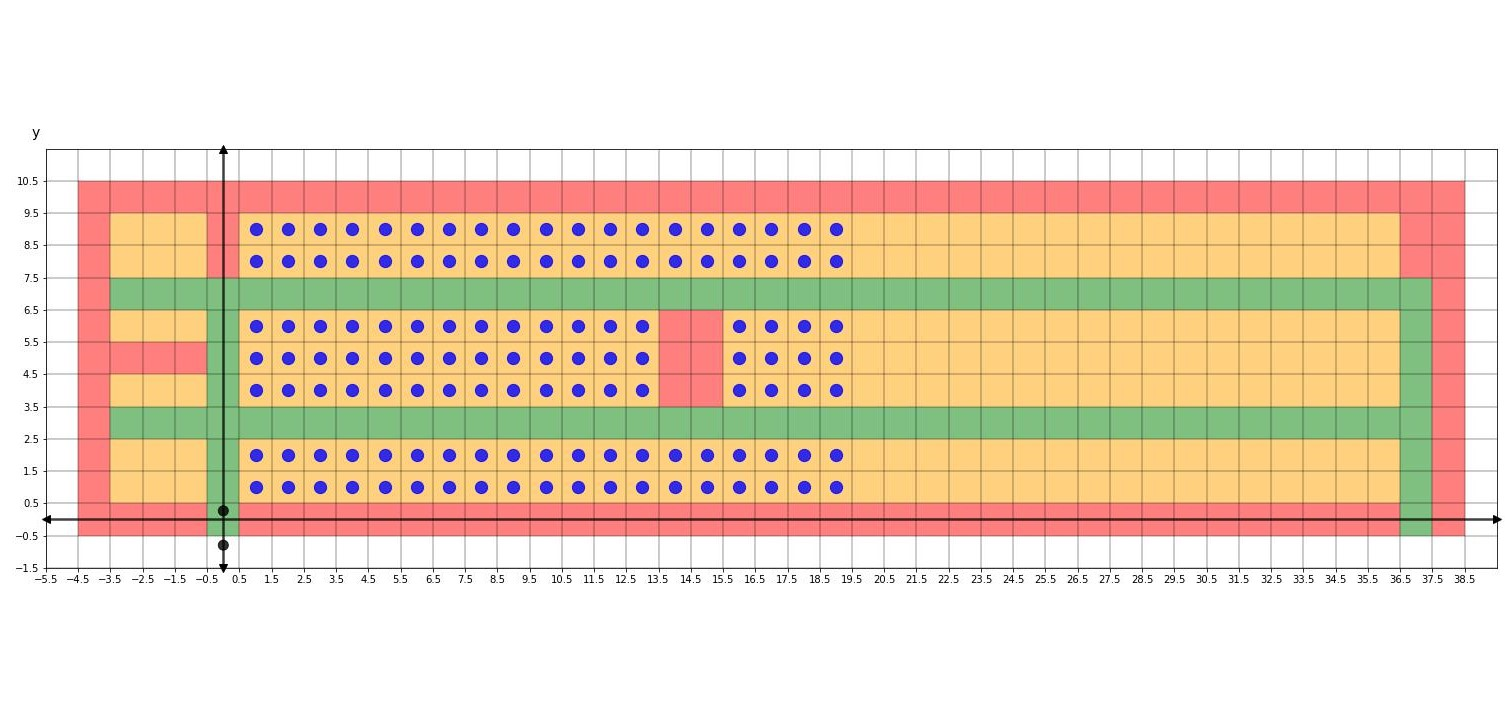
\includegraphics[width=14cm]{two1.jpg}\\
		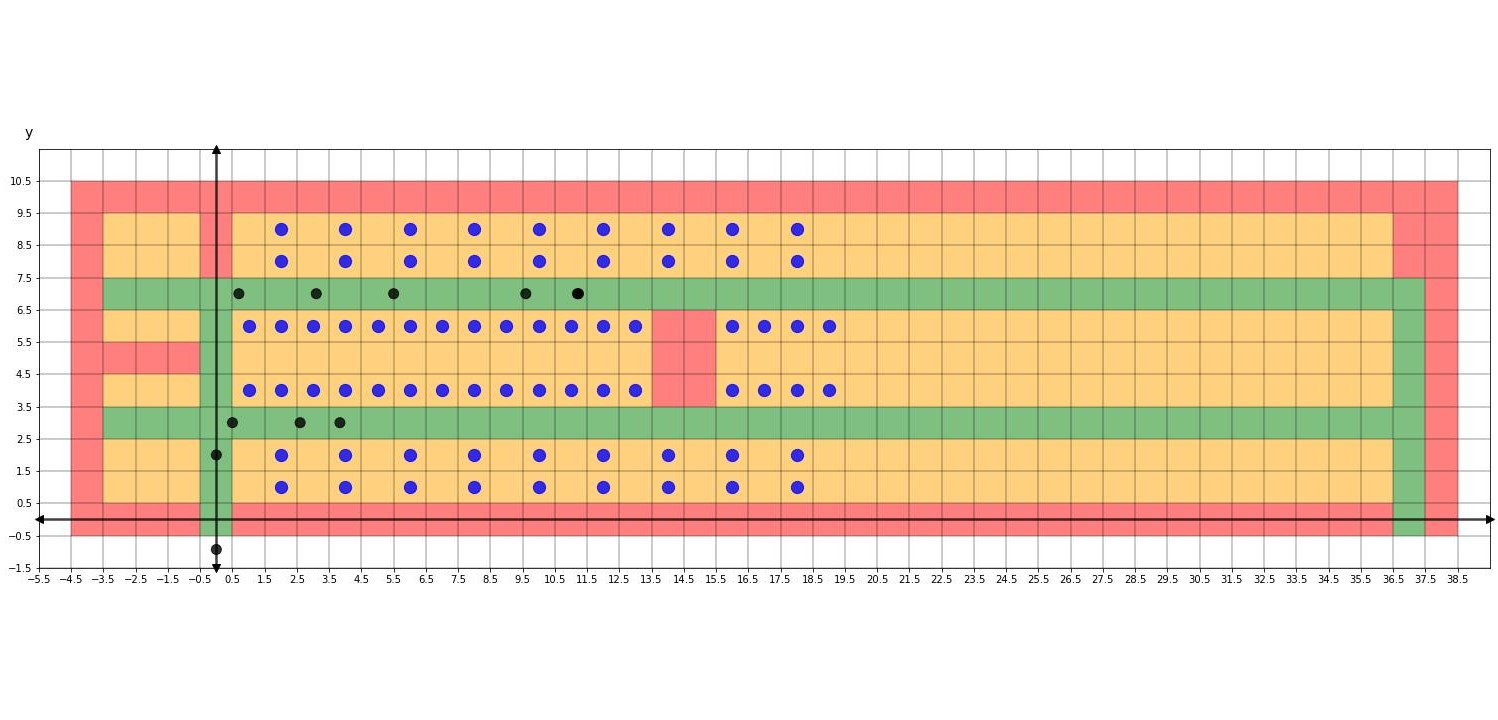
\includegraphics[width=14cm]{two2.jpg}\\
		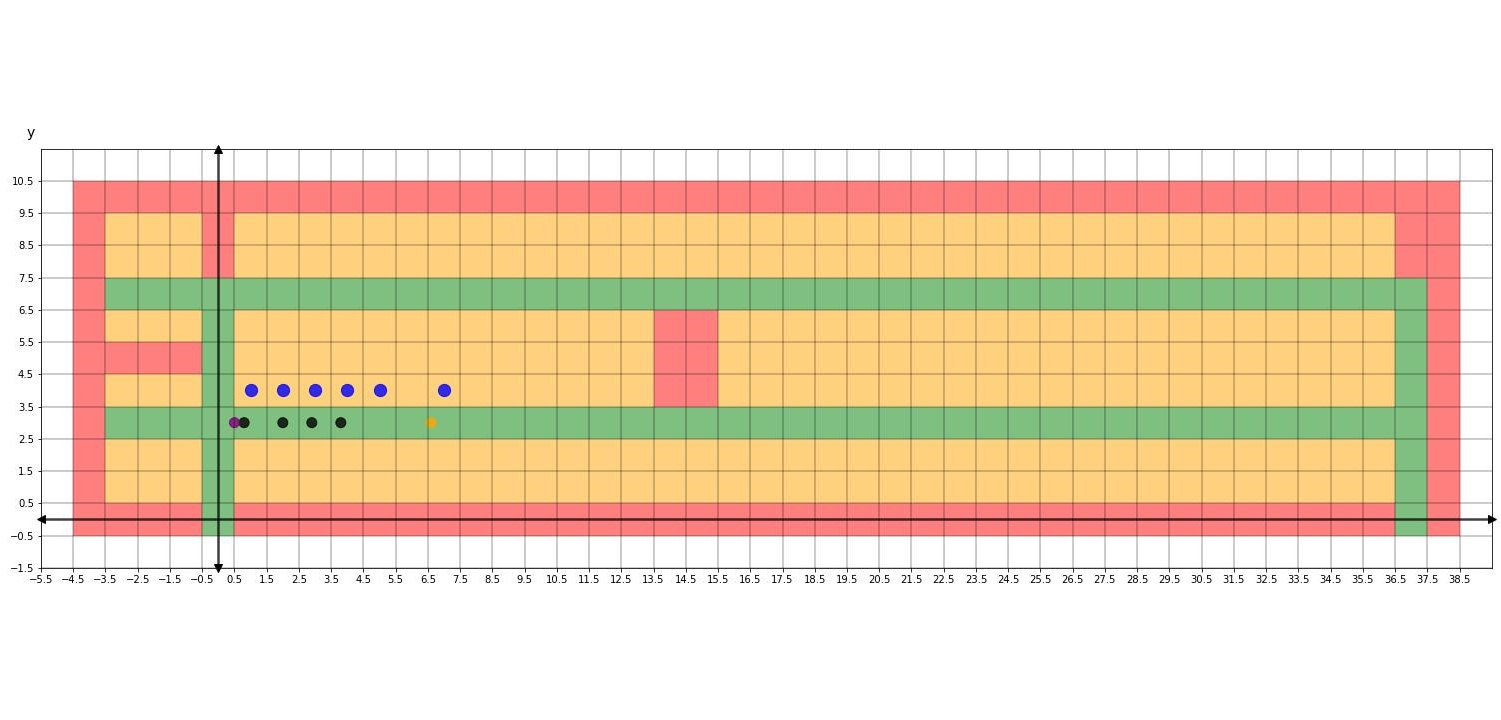
\includegraphics[width=14cm]{two3.jpg}\\
		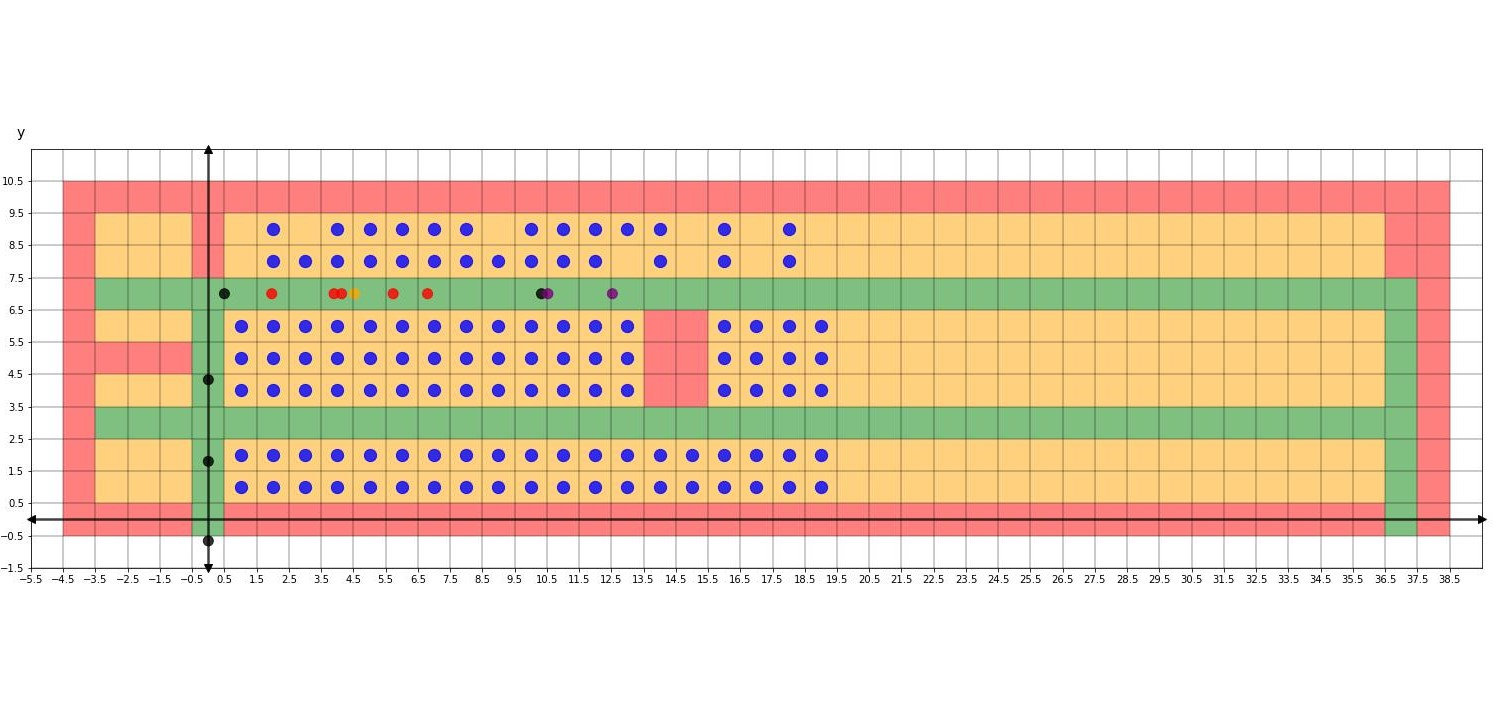
\includegraphics[width=14cm]{twobtf1.jpg}\\
		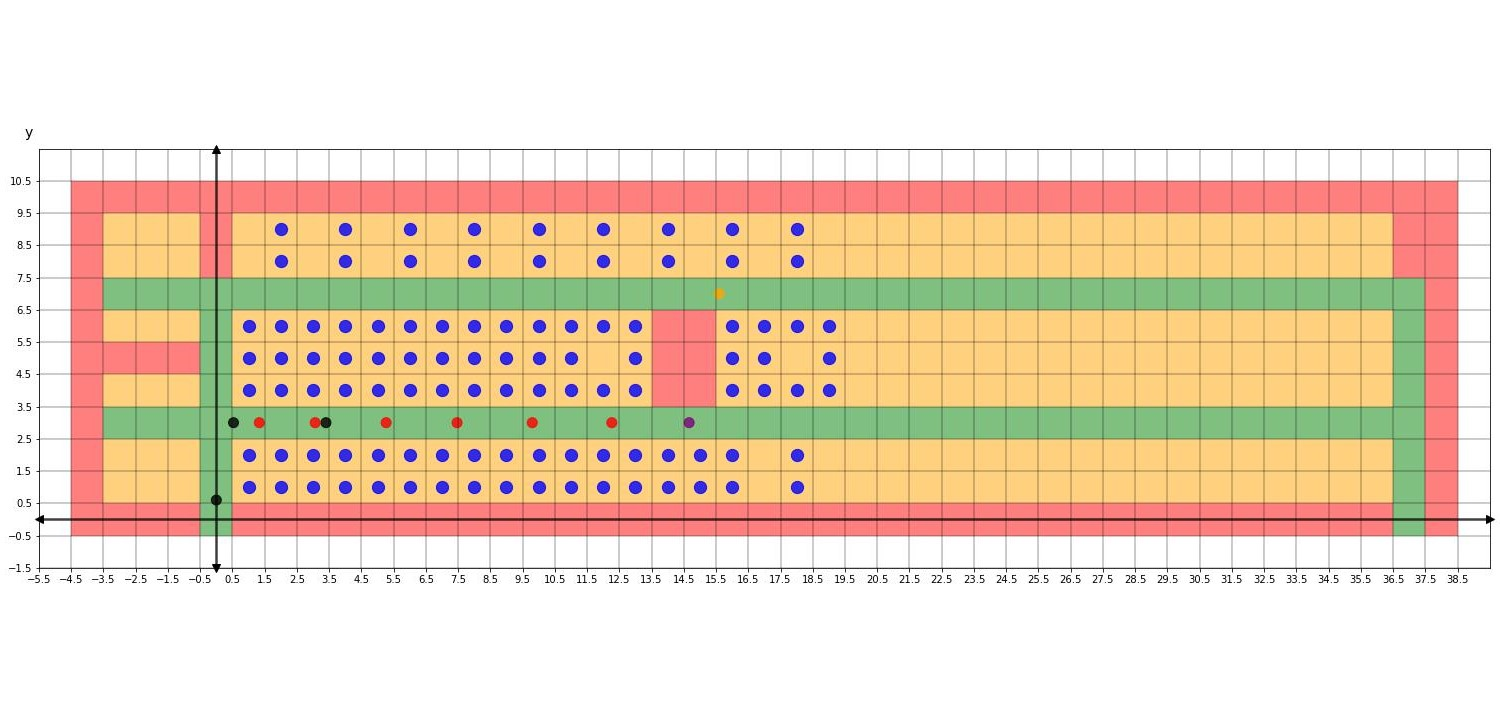
\includegraphics[width=14cm]{twobtf2.jpg}\\
		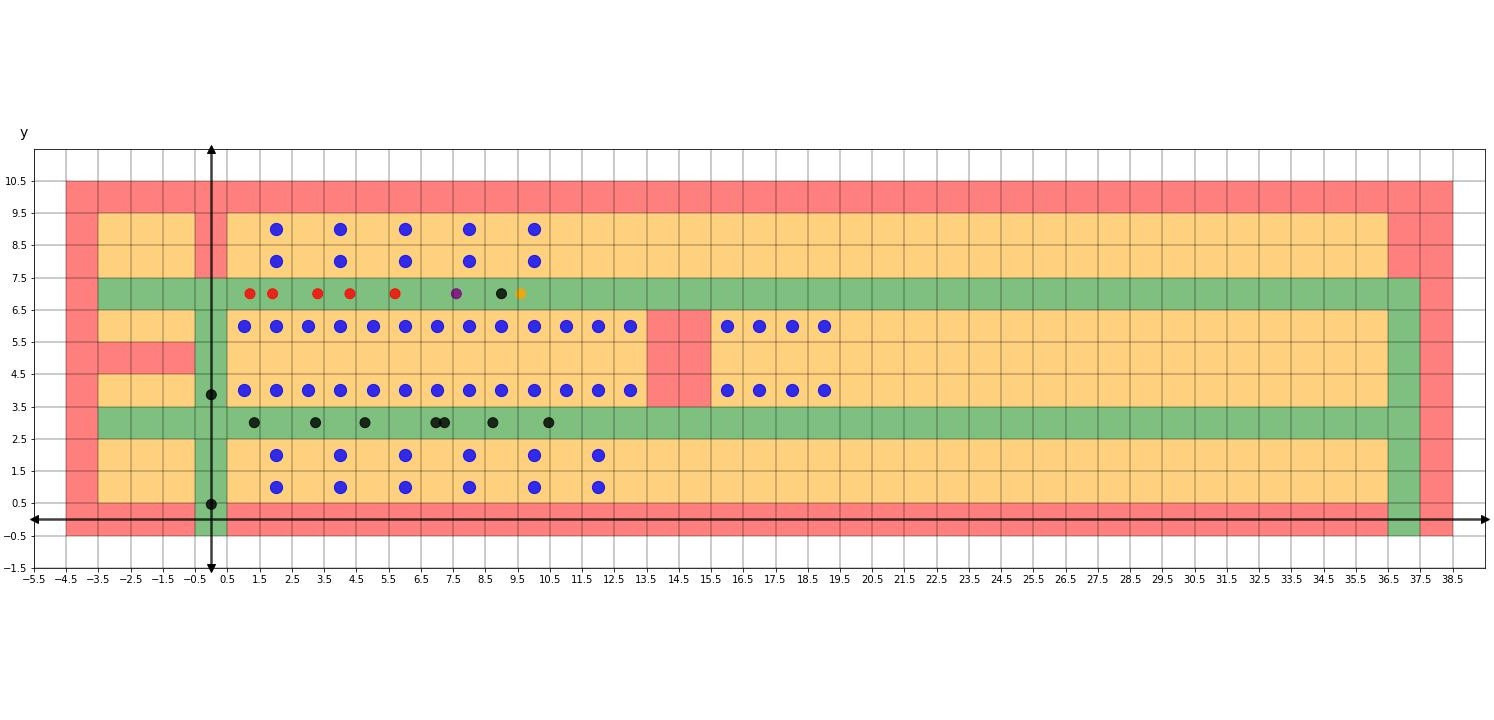
\includegraphics[width=14cm]{twobtf3.jpg}\\
	\end{center}
\end{document}
